\chapter{Results and Evaluation}
\label{chap:results}

This chapter presents the results of experimentation, and analysis of data obtained from the CardioSync Framework. Also it compares the key result outcomes of CardioSync framework, such as \textit{BLE connection setup time, power and energy consumption} in comparison to a naive and reference Freebie system that does not employ any synchronisation mechanism. 
\vspace{1\baselineskip}

\noindent The evaluation of the CardioSync framework is structured into three distinct contexts, inline with the research objectives
\begin{enumerate}
    \item Heart Rate Sensor Accuracy and Peak detection Algorithm performance.

    \item Verification of Integrated CardioSync framework in Continuous and Intermittent power.

    \item Comparative analysis of CardioSync Framework vs. Naive Reference FreeBie model.
\end{enumerate}

\section{Evaluation of Heart Rate Sensor and Peak detection Algorithm}
\label{sec:sensor_performance}
The evaluation in this section is split into two parts - \textit{Sensor accuracy profiling} based on phase difference for a particular peak detected between two sensors and \textit{BLE connection performance} at different sensor sampling rate.

\subsection{Sensor Accuracy Profiling}
Sensor accuracy to detect heart beat is mainly based on the peak detection algorithm, and also on the configurations of the sensor. However, the sensor was intentionally designed to function within a fixed configuration, optimising power consumption (Refer to Section:\ref{sec:sensor_config} in Appendix \ref{app:appendix_a}). So to quantitatively assess accuracy of the algorithm, the phase difference for heart pulse detection between two sensors was selected as the focus. This parameter was examined across various sampling rates of the peak detection algorithm.

\subsubsection{Experimental Setup}
To measure the phase difference between the heart pulse detected by two different MAX30102 sensors and a nRF52840DK development board \cite{nRF52840} was used. The measurement software was developed based on nRF5 SDK \cite{2023nRF5} to interface with two sensor boards using two-wire interface (TWI).  The software would use the heart beat detection algorithm of the CardioSync system to independently identify heart pulse peaks for each sensor and log the corresponding detection time. Subsequently, the phase difference should be computed between the aforementioned peaks. After two sensors have recorded around 250 peak detection, an experiment is finished, and it is repeated four times, each time with different sensor sampling rates: \textit{25Hz, 50Hz, 100Hz, and 1000Hz}.

\subsubsection{Results Discussion}
\begin{figure}[t]
    \begin{subfigure}{0.5\linewidth}
        \centering
        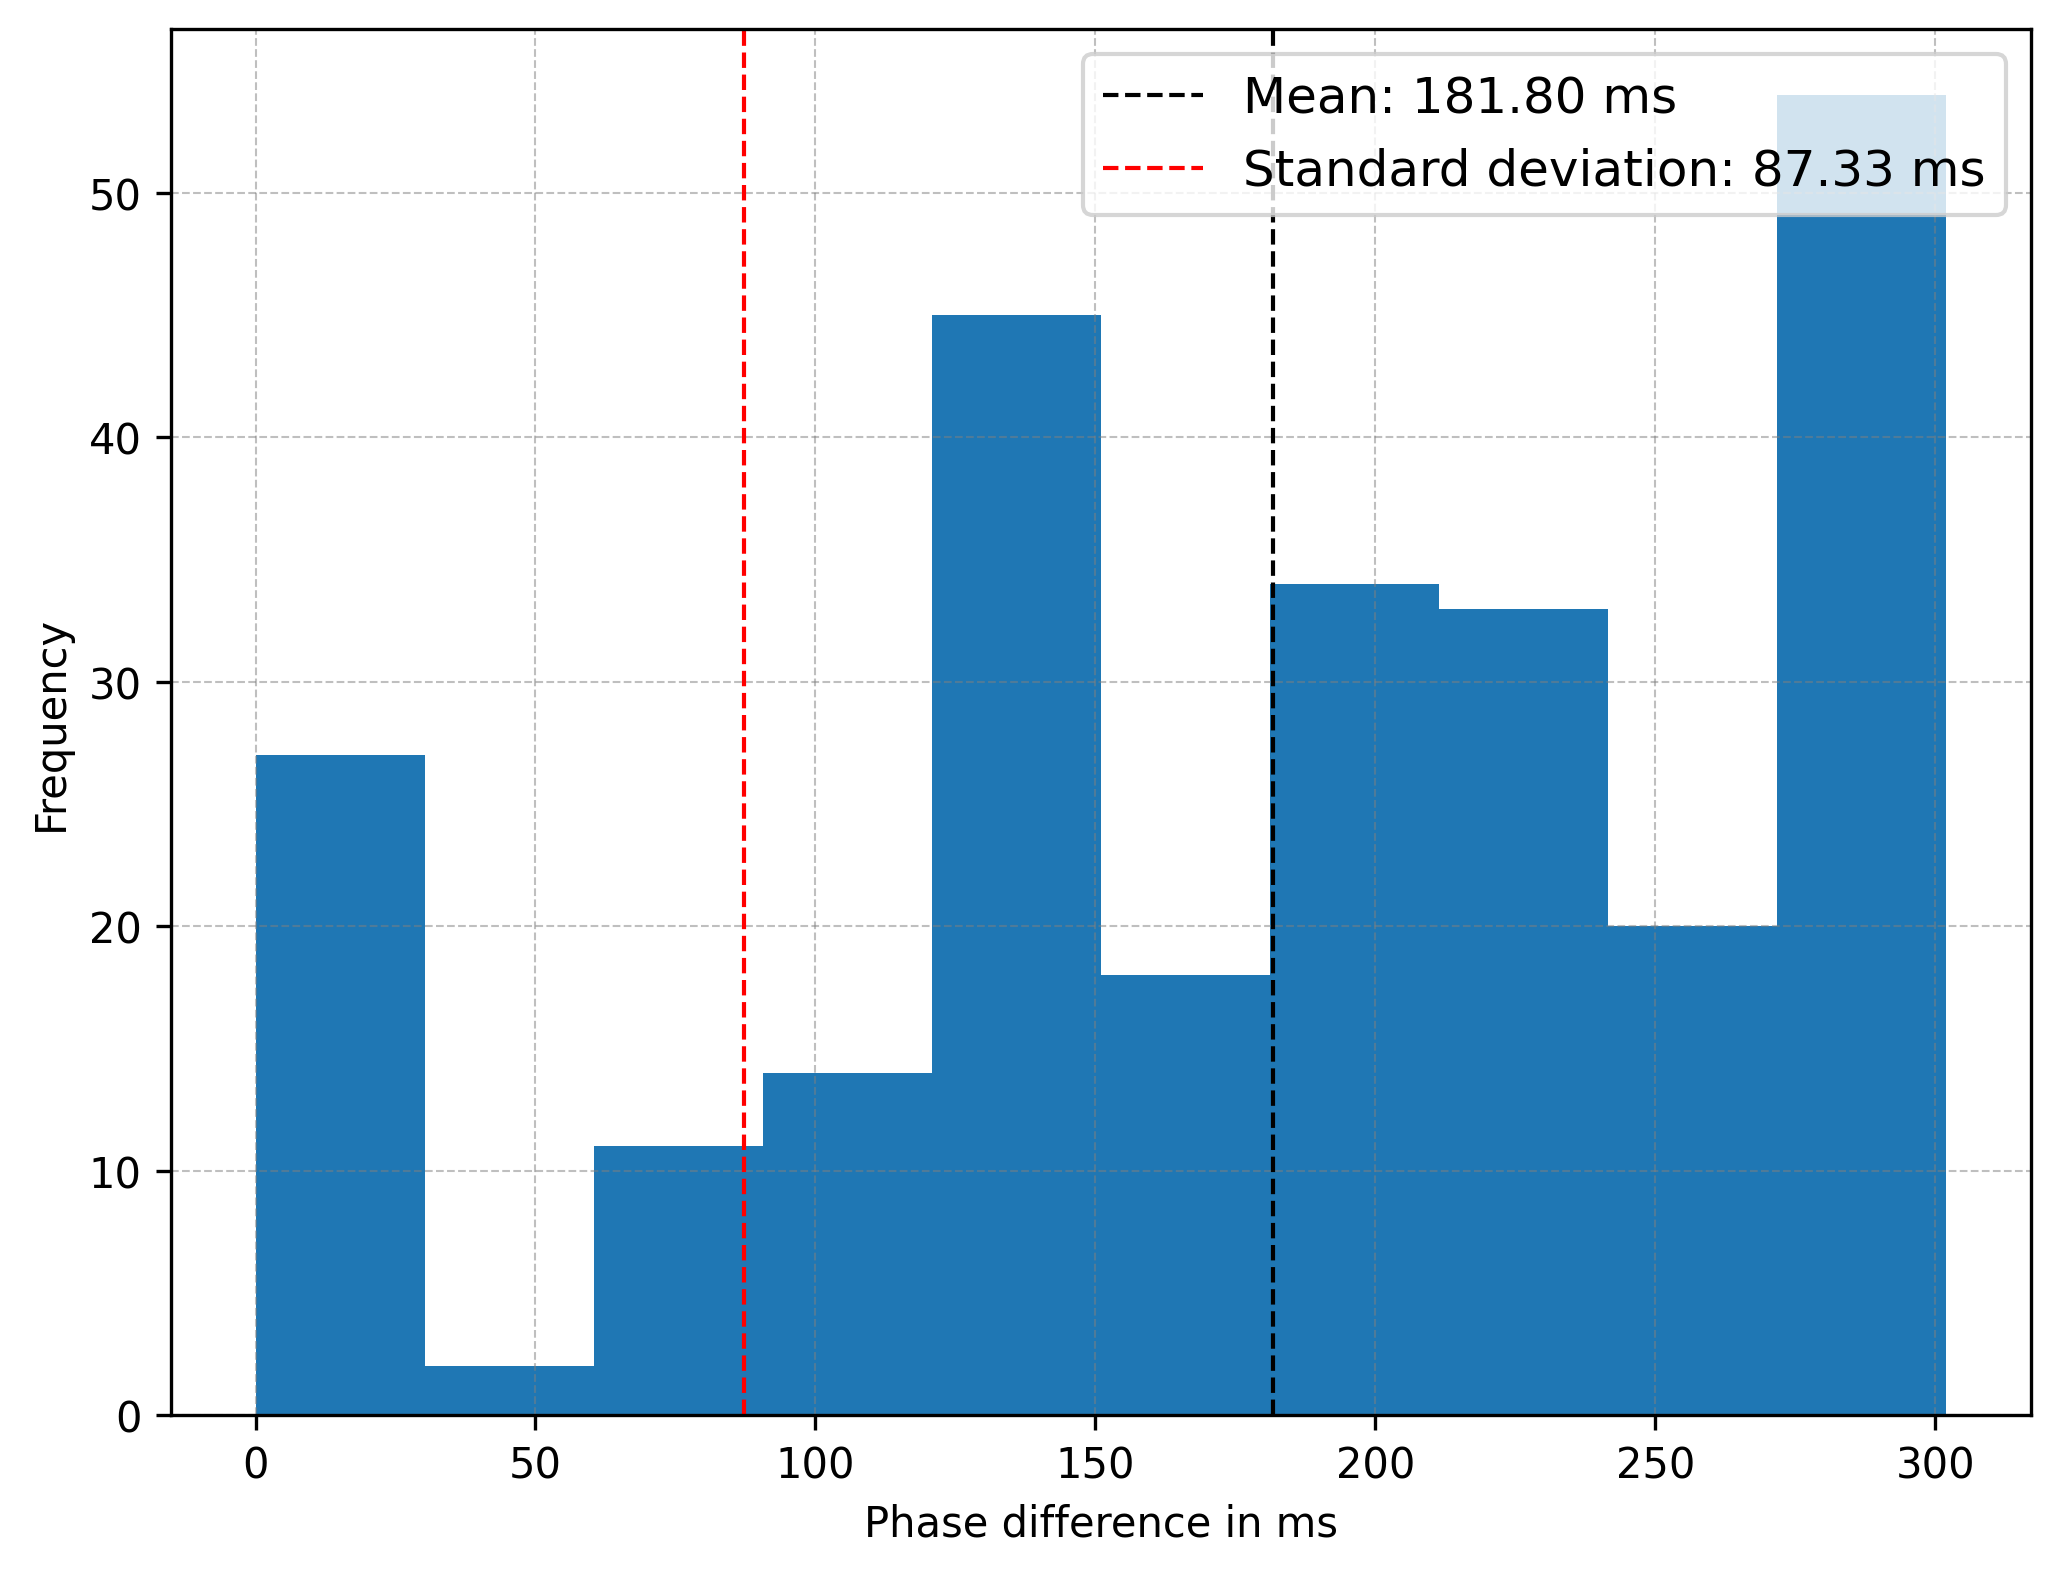
\includegraphics[width=\linewidth]{chapters/Results/histogram_25.png}
        \caption{25Hz}
        \label{fig:histogram_25}
        \vspace{1\baselineskip}
    \end{subfigure}
    \begin{subfigure}{0.5\linewidth}
        \centering
        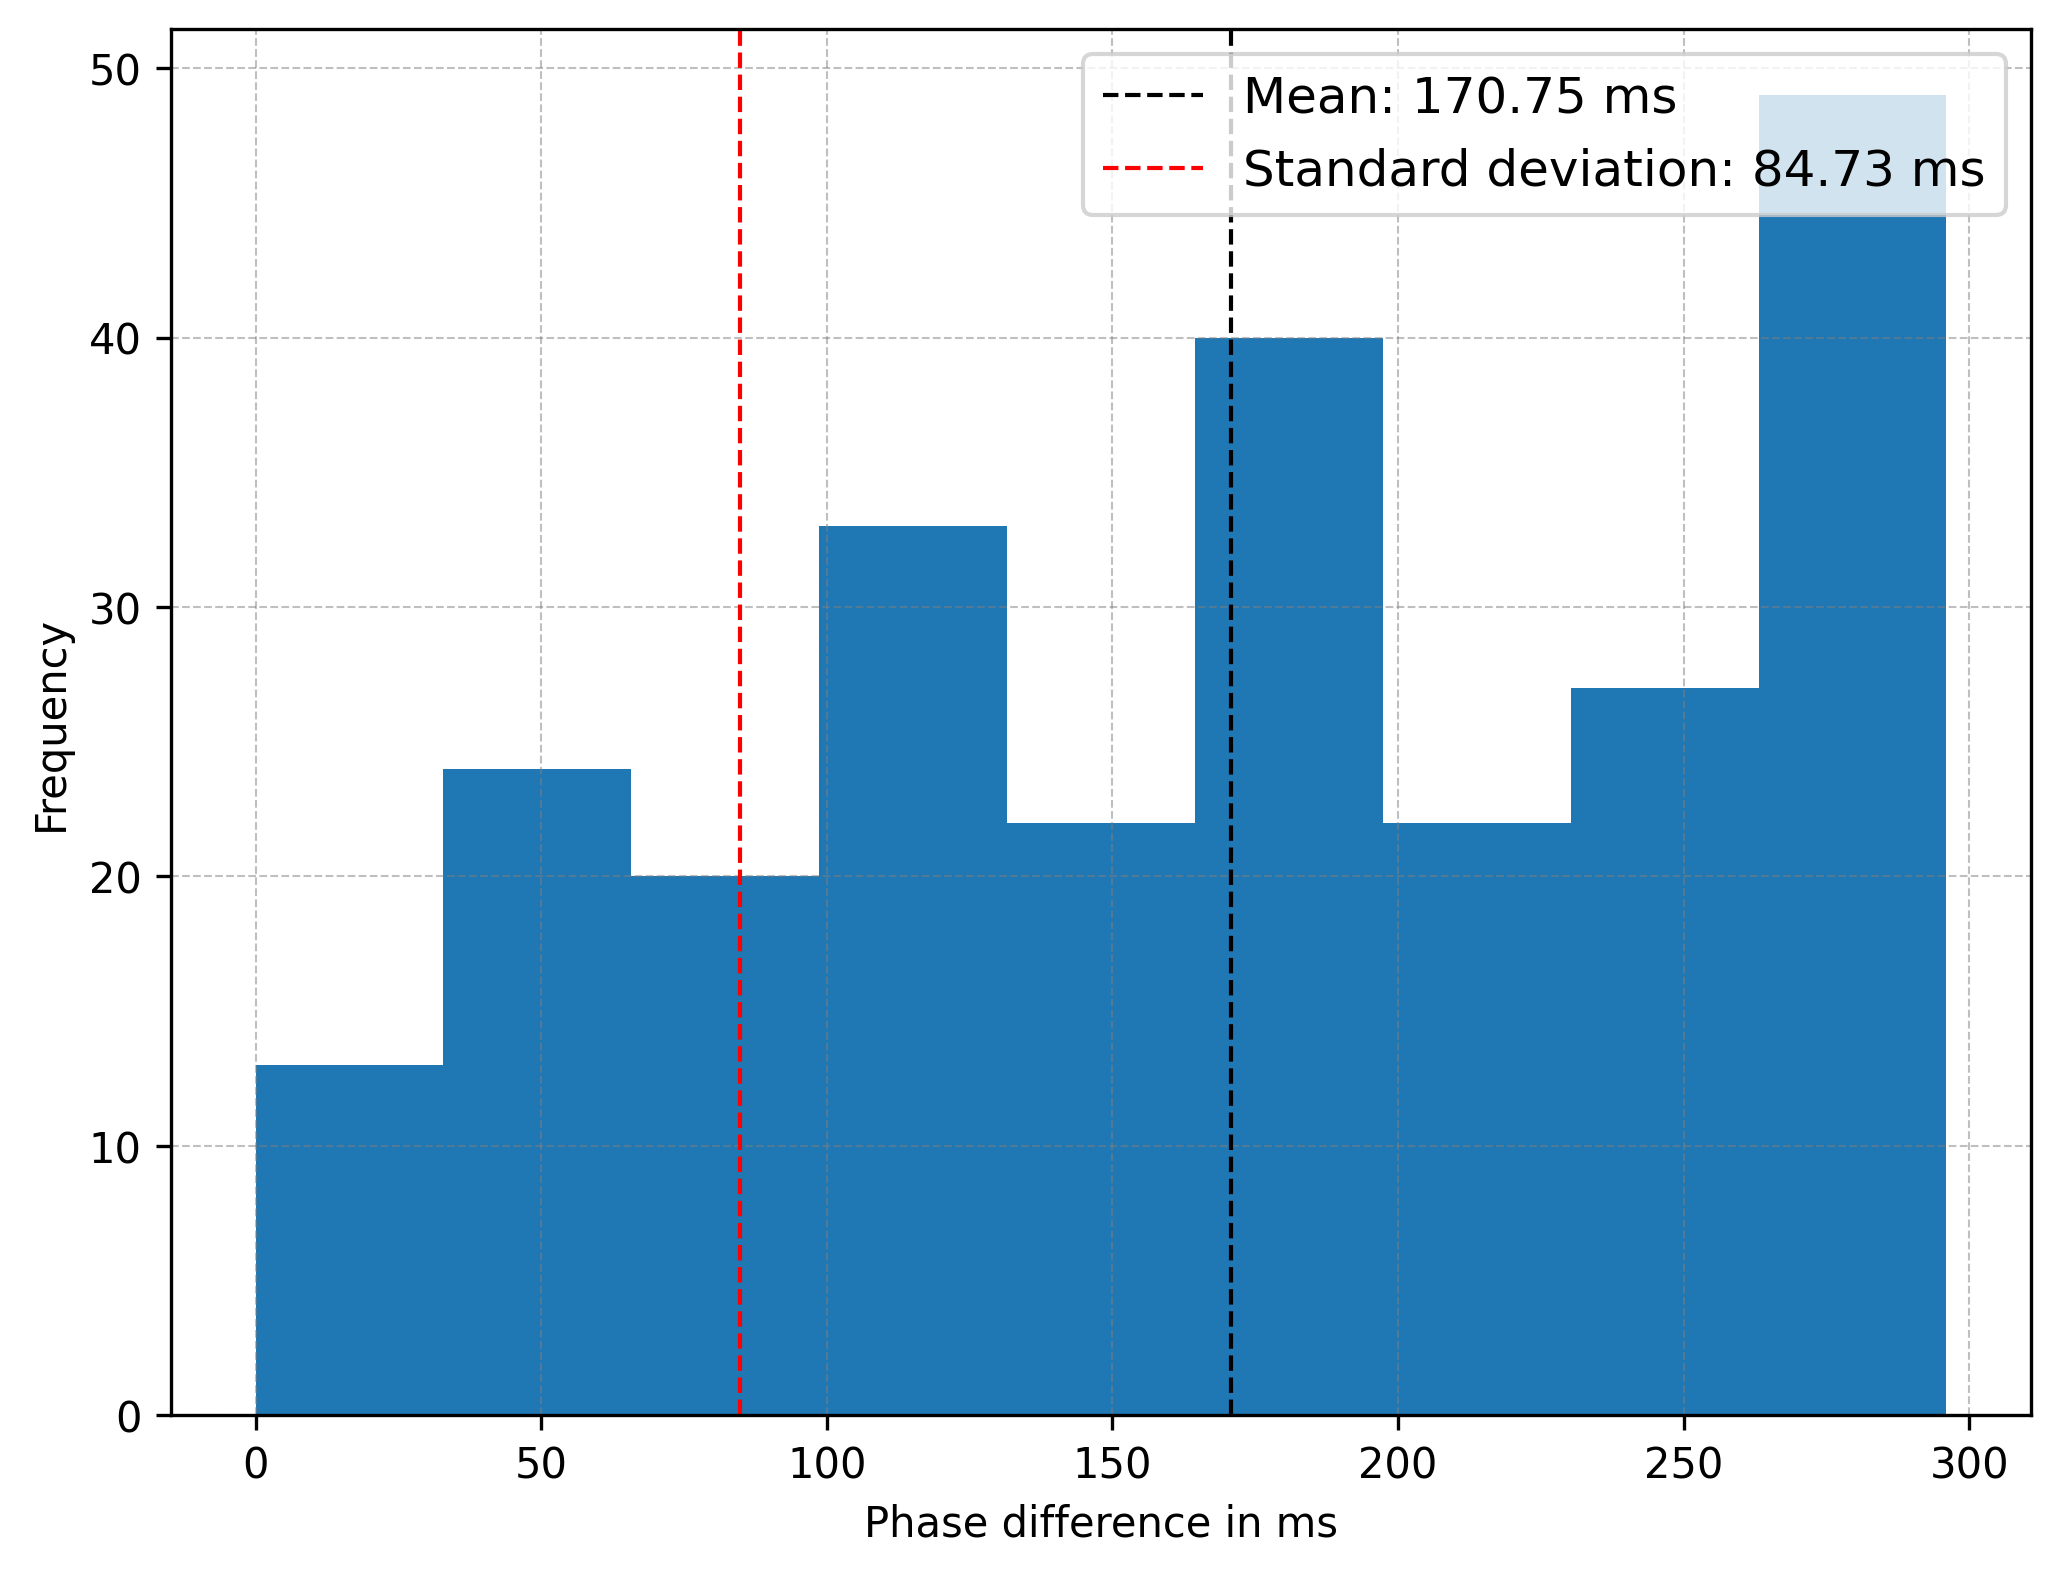
\includegraphics[width=\linewidth]{chapters/Results/histogram_50.png}
        \caption{50Hz}
        \label{fig:histogram_50}
        \vspace{1\baselineskip}
    \end{subfigure}
    \begin{subfigure}{0.5\linewidth}
        \centering
        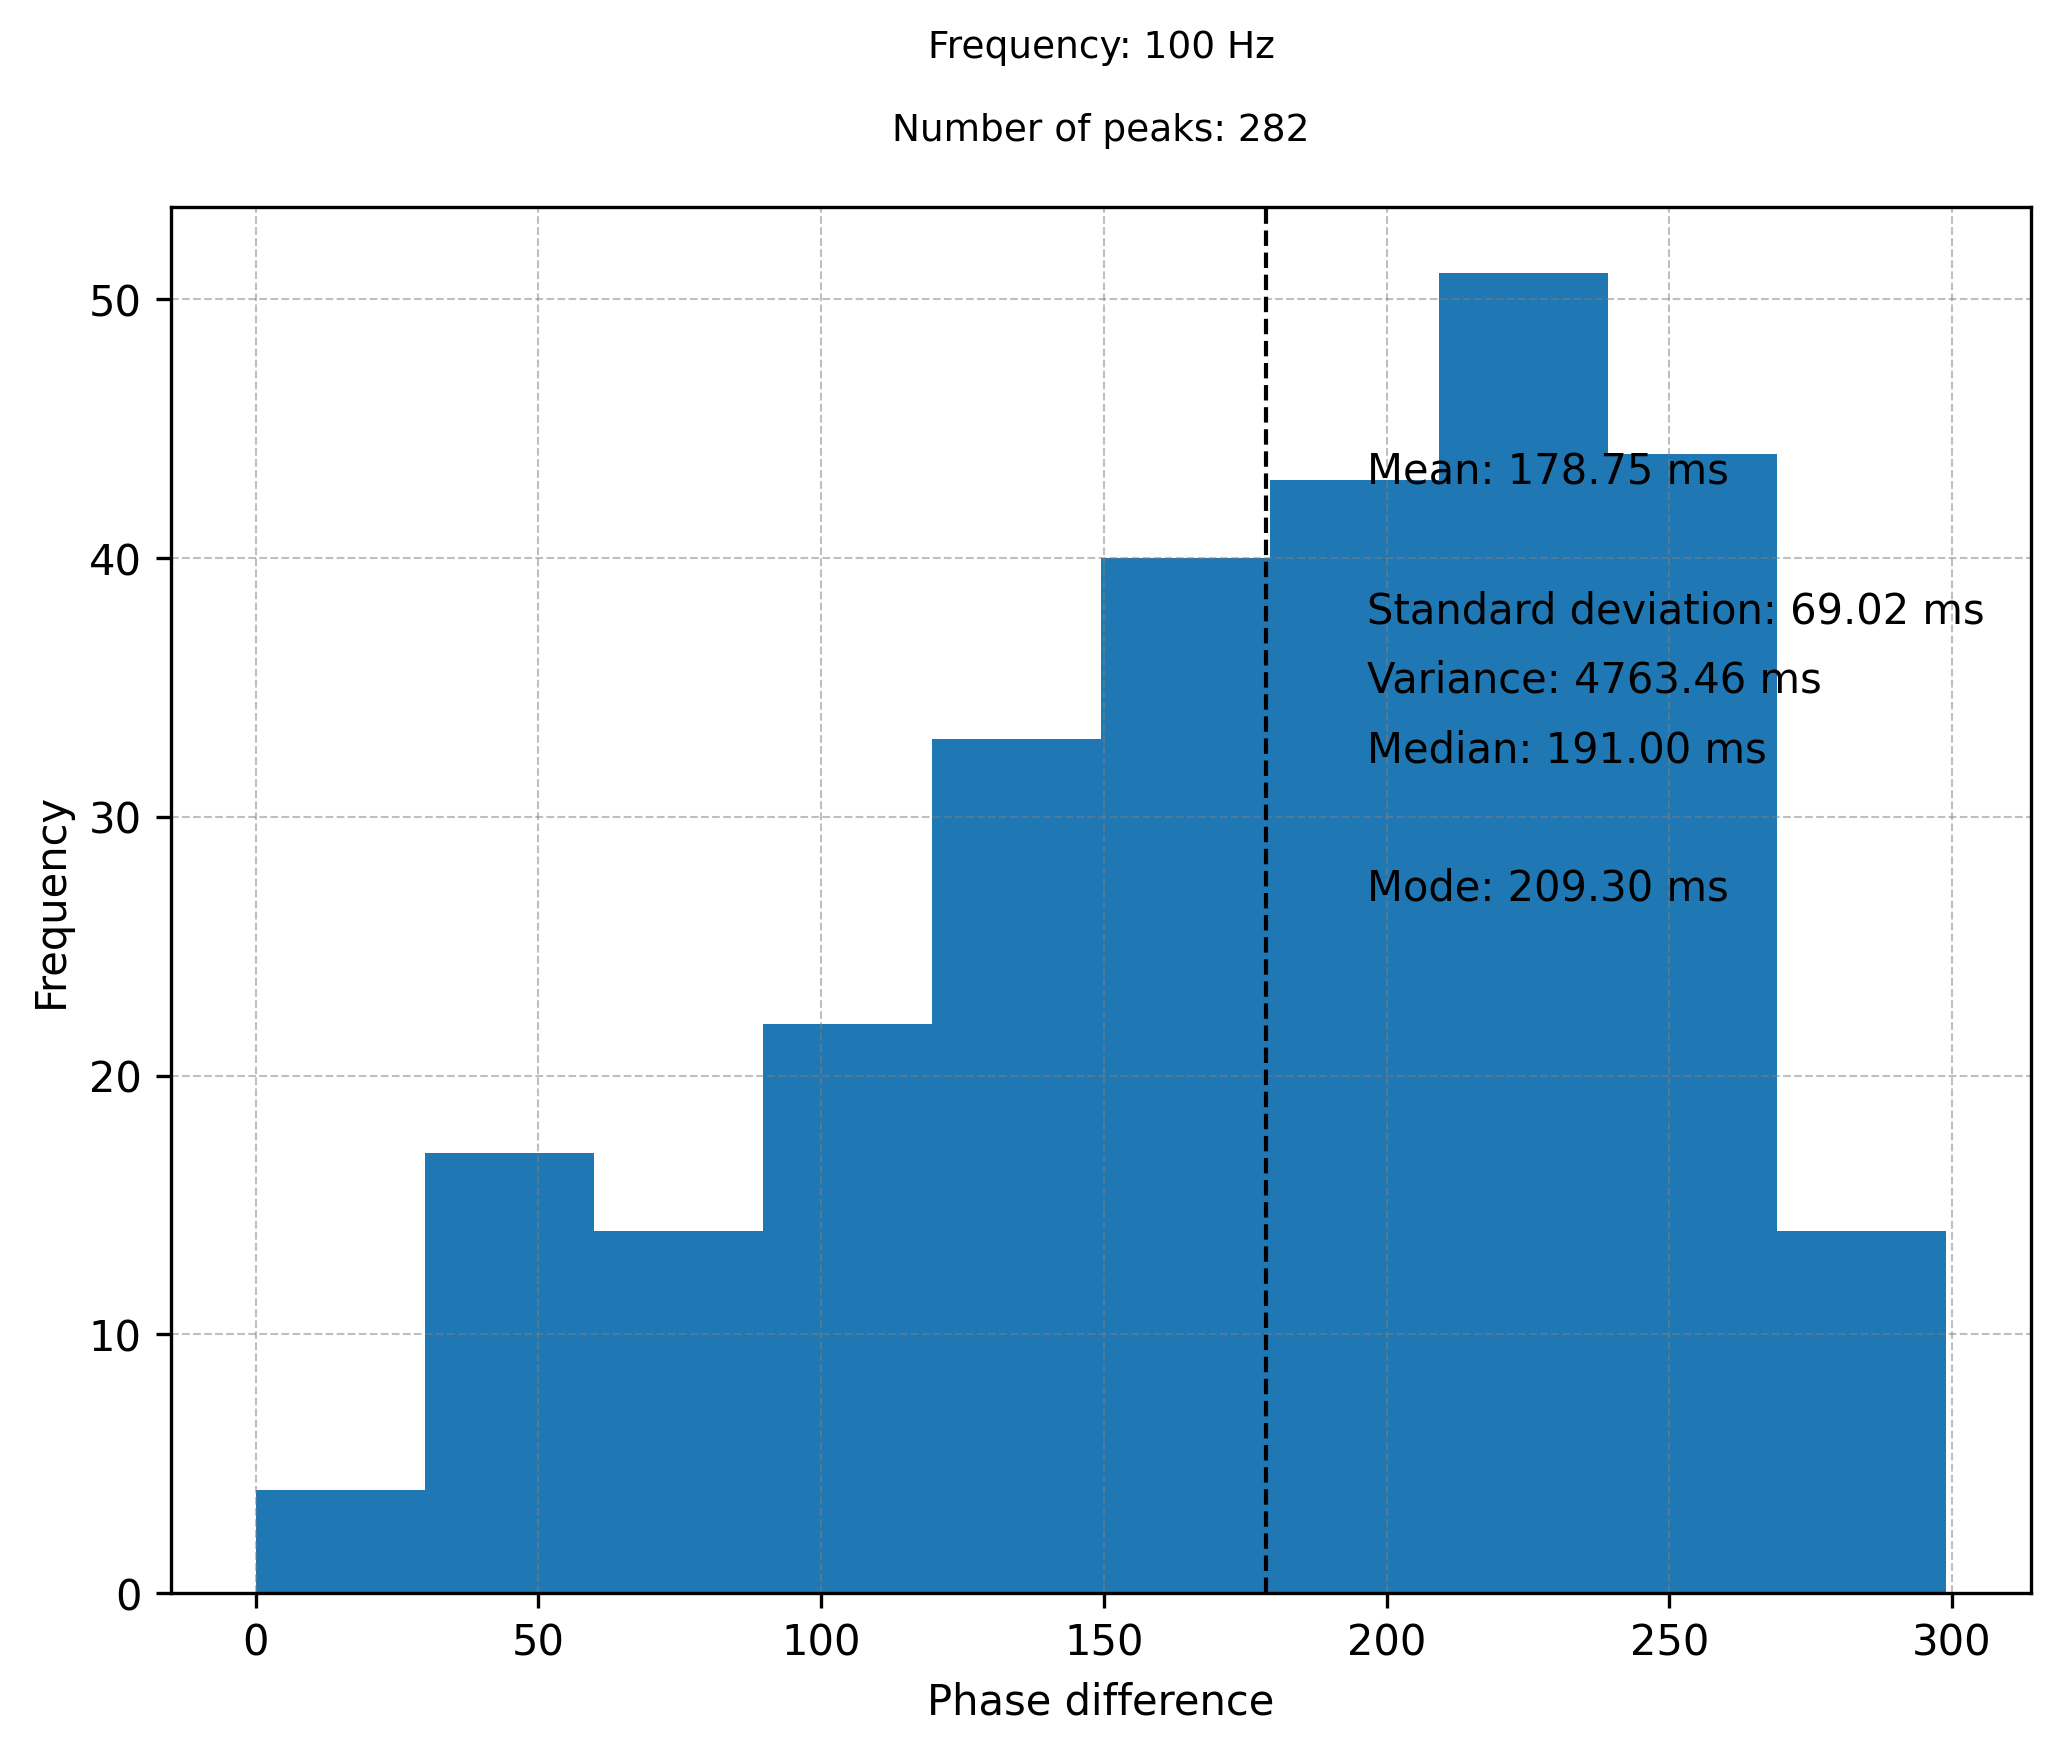
\includegraphics[width=\linewidth]{chapters/Results/histogram_100.png}
        \caption{100Hz}
        \label{fig:histogram_100}
    \end{subfigure}
    \begin{subfigure}{0.5\linewidth}
        \centering
        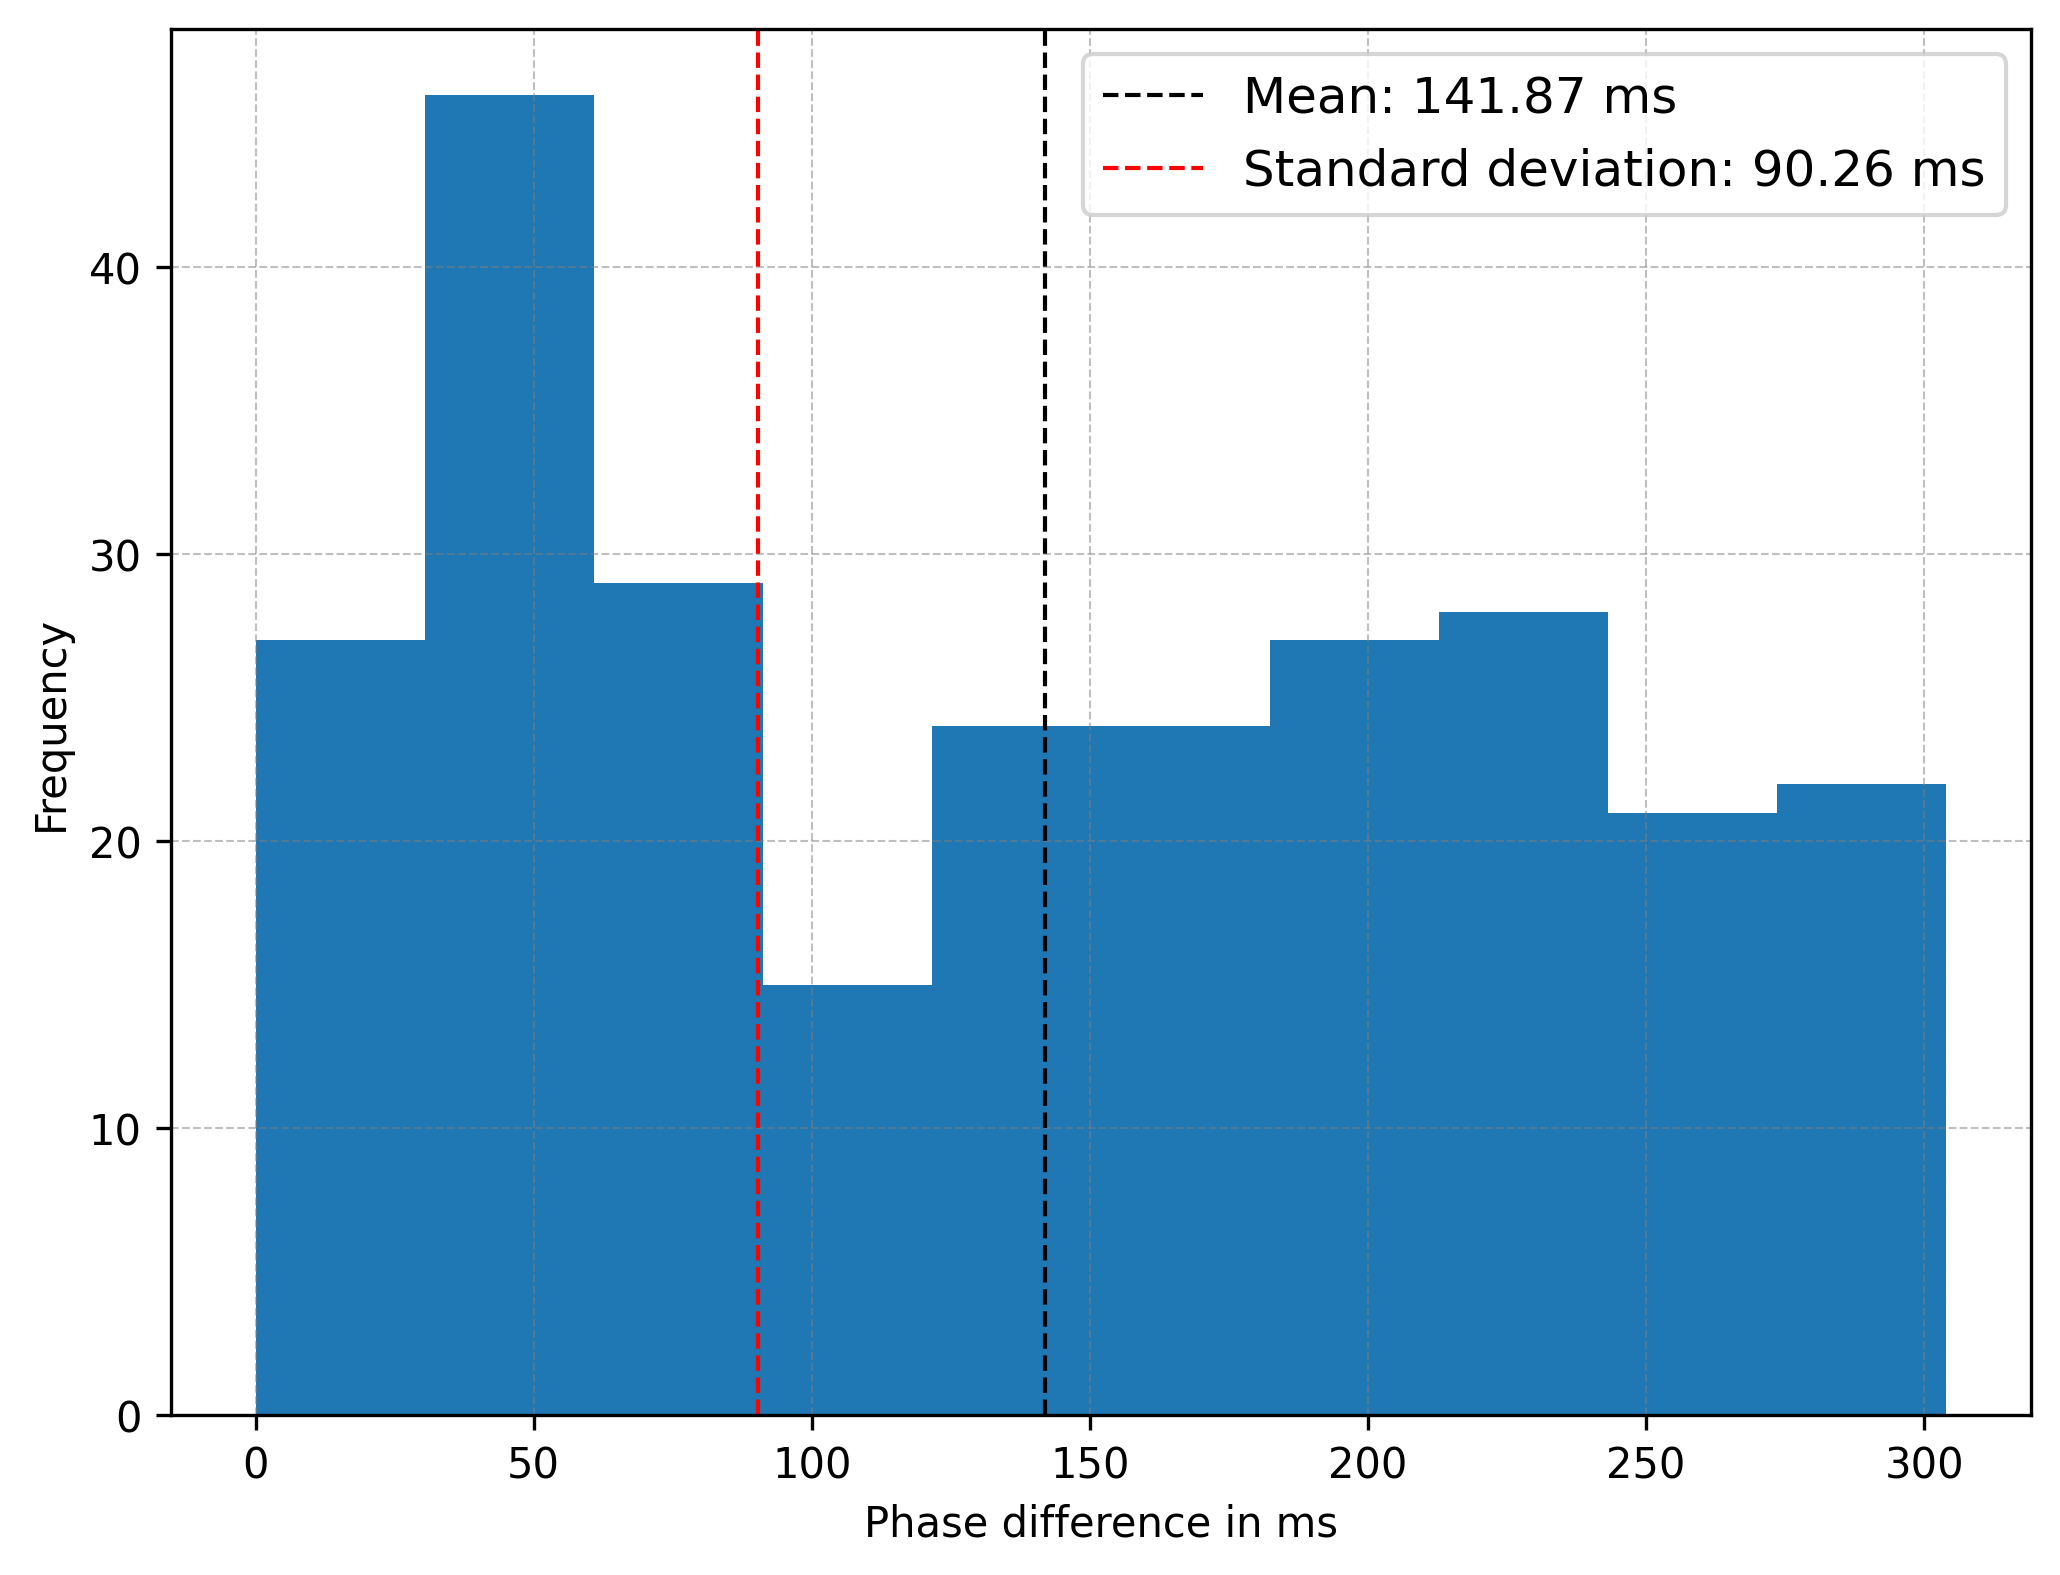
\includegraphics[width=\linewidth]{chapters/Results/histogram_1000.png}
        \caption{1000Hz}
        \label{fig:histogram_1000}
    \end{subfigure}
    \caption{Histograms of phase differences between heart pulses detected by two sensors at different sensor read frequencies. At 25 Hz and 50 Hz, larger phase differences occur at more frequency than 100 Hz. At 100 Hz, phase differences are evenly distributed around mean. At 100Hz, phases differences are more irregular.}
    \label{fig:histograms_sensor_accuracy}
\end{figure}

\begin{table}[t]
\centering
\begin{tabular}{|c|ccc|}
\hline
\multirow{2}{*}{\textbf{\begin{tabular}[c]{@{}c@{}}Sensor \\ Sampling rate\end{tabular}}} &
  \multicolumn{3}{c|}{\textbf{\begin{tabular}[c]{@{}c@{}}Phase difference\\ in milliseconds\end{tabular}}} \\ \cline{2-4} 
                 & \multicolumn{1}{c|}{\textbf{Mean}} & \multicolumn{1}{c|}{\textbf{Min}} & \textbf{Max} \\ \hline
25 Hz   & \multicolumn{1}{c|}{181.80}        & \multicolumn{1}{c|}{0}            & 301          \\ \hline
50 Hz   & \multicolumn{1}{c|}{170.75}        & \multicolumn{1}{c|}{0}            & 296          \\ \hline
100 Hz  & \multicolumn{1}{c|}{178.75}        & \multicolumn{1}{c|}{0}            & 299          \\ \hline
1000 Hz & \multicolumn{1}{c|}{141.87}        & \multicolumn{1}{c|}{0}            & 304          \\ \hline
\end{tabular}
\caption{Phase difference statistics at different sensor sampling rates.}
\label{tab:phase_difference_comp}
\end{table}

The histograms shown in Figure \ref{fig:histograms_sensor_accuracy} illustrate the distribution of phase differences recorded for various sensor sampling rates. The mean, minimum, and maximum phase differences are summarised in \autoref{tab:phase_difference_comp}. Analysing these distributions and their statistical characteristics reveals that phase difference in detection time between two sensors is inevitable. However, this data holds valuable insights for determining the optimal sensor read frequency for the CardioSync system.
\vspace{1\baselineskip}

\noindent At different sampling rates (25Hz, 50Hz, 100Hz, and 1000Hz), the distribution of phase differences between heart rate peaks reveals distinct characteristics. At 25Hz and 50Hz, a right-skewed distribution indicates a higher likelihood of larger phase differences, with about 33\% and 35\% of detected peaks respectively being more than 305ms out of phase. In contrast, a slightly right-skewed normal distribution at 100Hz suggests that phase differences mostly occur around the mean value, with around 24\% exceeding the 305ms threshold. A 1000Hz sampling rate presents an irregular phase difference distribution, highlighting unpredictable occurrences.
\vspace{1\baselineskip}

\noindent From all these observations, it can be concluded that \textbf{\textbf{Sampling rate 100Hz}} is more predictable in terms of phase difference and is more accurate in heart pulse peak detection between two sensors. Also, even the sensor settings are at 50 samples per second, thereby not losing any samples from the sensor.



\subsection{BLE connection performance}

\noindent The aim of this assessment is to analyse the performance of the novel CardioSync peak detection algorithm with the synchronised Bluetooth Low Energy (BLE) connection at different sensor sampling rates. This evaluation is conducted in preparation for the integration of the algorithm into the FreeBie architecture. The analysis was based on the number of peaks needed for successful connection establishment.

\subsubsection{Experimental Setup}
To record the number of heart pulse peaks needed for successful BLE connection, two nRF52840DK development board \cite{nRF52840} were used and each board was interfaced with one MAX30102 sensor \cite{2018MAX30102} to its I2C GPIO pins. Measurement software was developed based on the PacketCraft BLE stack \cite{2020Packetcraft}. The devised measurement code calculates the average time interval between peaks detected by the algorithm in run time. Also once the connection is established, it records the number of peaks detected before connection.
\vspace{1\baselineskip}

\noindent With these setup, 15 experiments were performed at different sensor sampling frequencies. Each experiment is considered complete once the connection is established between two nRF52840DK boards using the MAX30102 detected heart pulses.

\subsubsection{Results Discussion}

\begin{table}[t]
\centering
\begin{tabular}{|c|cc|cc|}
\hline
\multirow{2}{*}{\textbf{\begin{tabular}[c]{@{}c@{}}Sensor \\ Sampling rate\end{tabular}}} &
  \multicolumn{2}{c|}{\textbf{\begin{tabular}[c]{@{}c@{}}Average number \\ of peaks detected \\ to connect\end{tabular}}} &
  \multicolumn{2}{c|}{\textbf{\begin{tabular}[c]{@{}c@{}}Average\\ Connection setup time\\ in seconds\end{tabular}}} \\ \cline{2-5} 
                 & \multicolumn{1}{c|}{\textbf{Peripheral}} & \textbf{Central} & \multicolumn{1}{c|}{\textbf{Peripheral}} & \textbf{Central} \\ \hline
50 Hz   & \multicolumn{1}{c|}{1.6}                 & 1.6              & \multicolumn{1}{c|}{2.789}               & 2.847            \\ \hline
100 Hz  & \multicolumn{1}{c|}{1.667}               & 1.733            & \multicolumn{1}{c|}{2.074}               & 2.018            \\ \hline
1000 Hz & \multicolumn{1}{c|}{1.8667}              & 1.733            & \multicolumn{1}{c|}{1.407}               & 1.129            \\ \hline
\end{tabular}
\caption{Comparison of BLE connection at different sensor sampling rates. Number of peaks detected before connection setup occurs is lesser at 100 Hz than 1000 Hz, even though the average connection setup time is lower at 1000 Hz.}
\label{tab:ble_conn_comp}
\end{table}


\begin{table}[t]
\centering
\begin{tabular}{|cc|}
\hline
\multicolumn{2}{|c|}{\textbf{\begin{tabular}[c]{@{}c@{}}BLE Advertisement Parameters\\ (Peripheral)\end{tabular}}} \\ \hline
\multicolumn{1}{|c|}{\textit{Advertising Interval}} & 50 milliseconds  \\ \hline
\multicolumn{1}{|c|}{\textit{Advertising Duration}} & 200 milliseconds \\ \hline
\multicolumn{2}{|c|}{\textbf{\begin{tabular}[c]{@{}c@{}}BLE Scan Parameters\\ (Central)\end{tabular}}}             \\ \hline
\multicolumn{1}{|c|}{\textit{Scan Interval}}        & 15 milliseconds  \\ \hline
\multicolumn{1}{|c|}{\textit{Scan Window}}          & 20 milliseconds  \\ \hline
\multicolumn{1}{|c|}{\textit{Scan Duration}}        & 200 milliseconds \\ \hline
\end{tabular}
\caption{Chosen BLE parameters for the CardioSync system based on chosen sampling rate 100 Hz.}
\label{tab:ble_params}
\end{table}

The results in \autoref{tab:ble_conn_comp} demonstrate that a sampling frequency of 1000Hz results in a shorter average time interval between peaks, enhancing connection establishment time due to quicker peak detection. However, this frequency exhibited an inconsistent number of peaks between experiments for connection establishment, leading to a higher average number of required peaks. Consequently, balancing these findings with the earlier assessment of sensor accuracy, \textbf{the 100Hz sampling rate was selected for integrating the CardioSync system}.
\vspace{1\baselineskip}

\noindent Furthermore, the selection of a sample frequency of 100Hz has led to the determination of BLE parameters for the CardioSync system, backed up by the outcomes of this evaluation. In order to address the \textbf{average phase difference of 178.75 milliseconds} observed between two sensors and reducing the number of peaks necessary to establish a connection, the BLE advertising and scanning configurations have been chosen as outlined in Table \ref{tab:ble_params}. 
\vspace{1\baselineskip}

\noindent Both the scan and advertising duration have been set at 200 milliseconds for each detected heart pulse. This allows for a sufficient window of time to synchronise and establish a connection, even in cases where there may be a significant disparity between the readings from two sensors.


\section{Validation of Integrated CardioSync System}
The purpose of the following section is to provide an illustration of the operational functionality of the integrated CardioSync framework to synchronise a BLE connection setup within sleep-wakeup principles of the FreeBie system architecture. The findings are presented for two types of input power: Continuous power and Intermittent power (which were emulated using a square wave and the parameters of the square wave are 75\% duty cycle and total period of 8 seconds).

\subsection{Experimental Setup}
\label{sec:experimental_setup}
\subsubsection{Hardware Setup}
The experimental configuration comprises of two FreeBie boards \cite{Researchers}, each equipped with a MAX30102 sensor. The voltage supplied to the sensor is derived from the \(\text{V}_\text{Batt}\) source on the FreeBie board. The FreeBie board receives its voltage supply from a voltage emulator kit called \textit{DIPS} \cite{DIPSGitHub} connected to the \(\text{V}_\text{Store}\) pin. The DIPS system comes with Emulator Host software, which facilitates the configuration and simulation of the desired voltage supply for the FreeBie system \cite{DIPSGitHub}.
\vspace{1\baselineskip}

\noindent The \textit{Saleae logic analyser} \cite{LogicAnalyser} is employed to gather results that demonstrate the functionality of the system. In our experimental setup, we employed four channels from logic analyser for each of the FreeBie boards to measure the voltage values of \textit{\(\text{V}_\text{DD\_MCU}\), \(\text{V}_\text{Store}\), Sensor Read state(GPIO pin), and Connection Open indication (GPIO pin)}.
\vspace{1\baselineskip}

\noindent The \textit{nRF Power Profiler Kit II (PPK)} \cite{2023Power} is employed for the purpose of measuring energy consumption throughout the runtime by hooking it to the \(\text{V}_\text{Store}\) pin of the board. Additionally, it serves as a continuous source of power for the FreeBie board. Similar to the Saleae Logic analyser, the PPK is capable of capturing and recording current measurements of a device in real-time.

\subsubsection{Software Setup}
Regarding the experimental software setup, modifications have been made to the system described in Chapter \ref{chap:implementation}. These modifications involve the activation of two GPIO pins to indicate the start and stop of the sensor read phase and the successful establishment of a BLE connection respectively. One of the FreeBie board is programmed with the CardioSync Peripheral code, while the other is flashed with the CardioSync Central code.

\subsection{Results Discussion}

\begin{figure}[ht]
    \begin{subfigure}{1\linewidth}
        \centering
        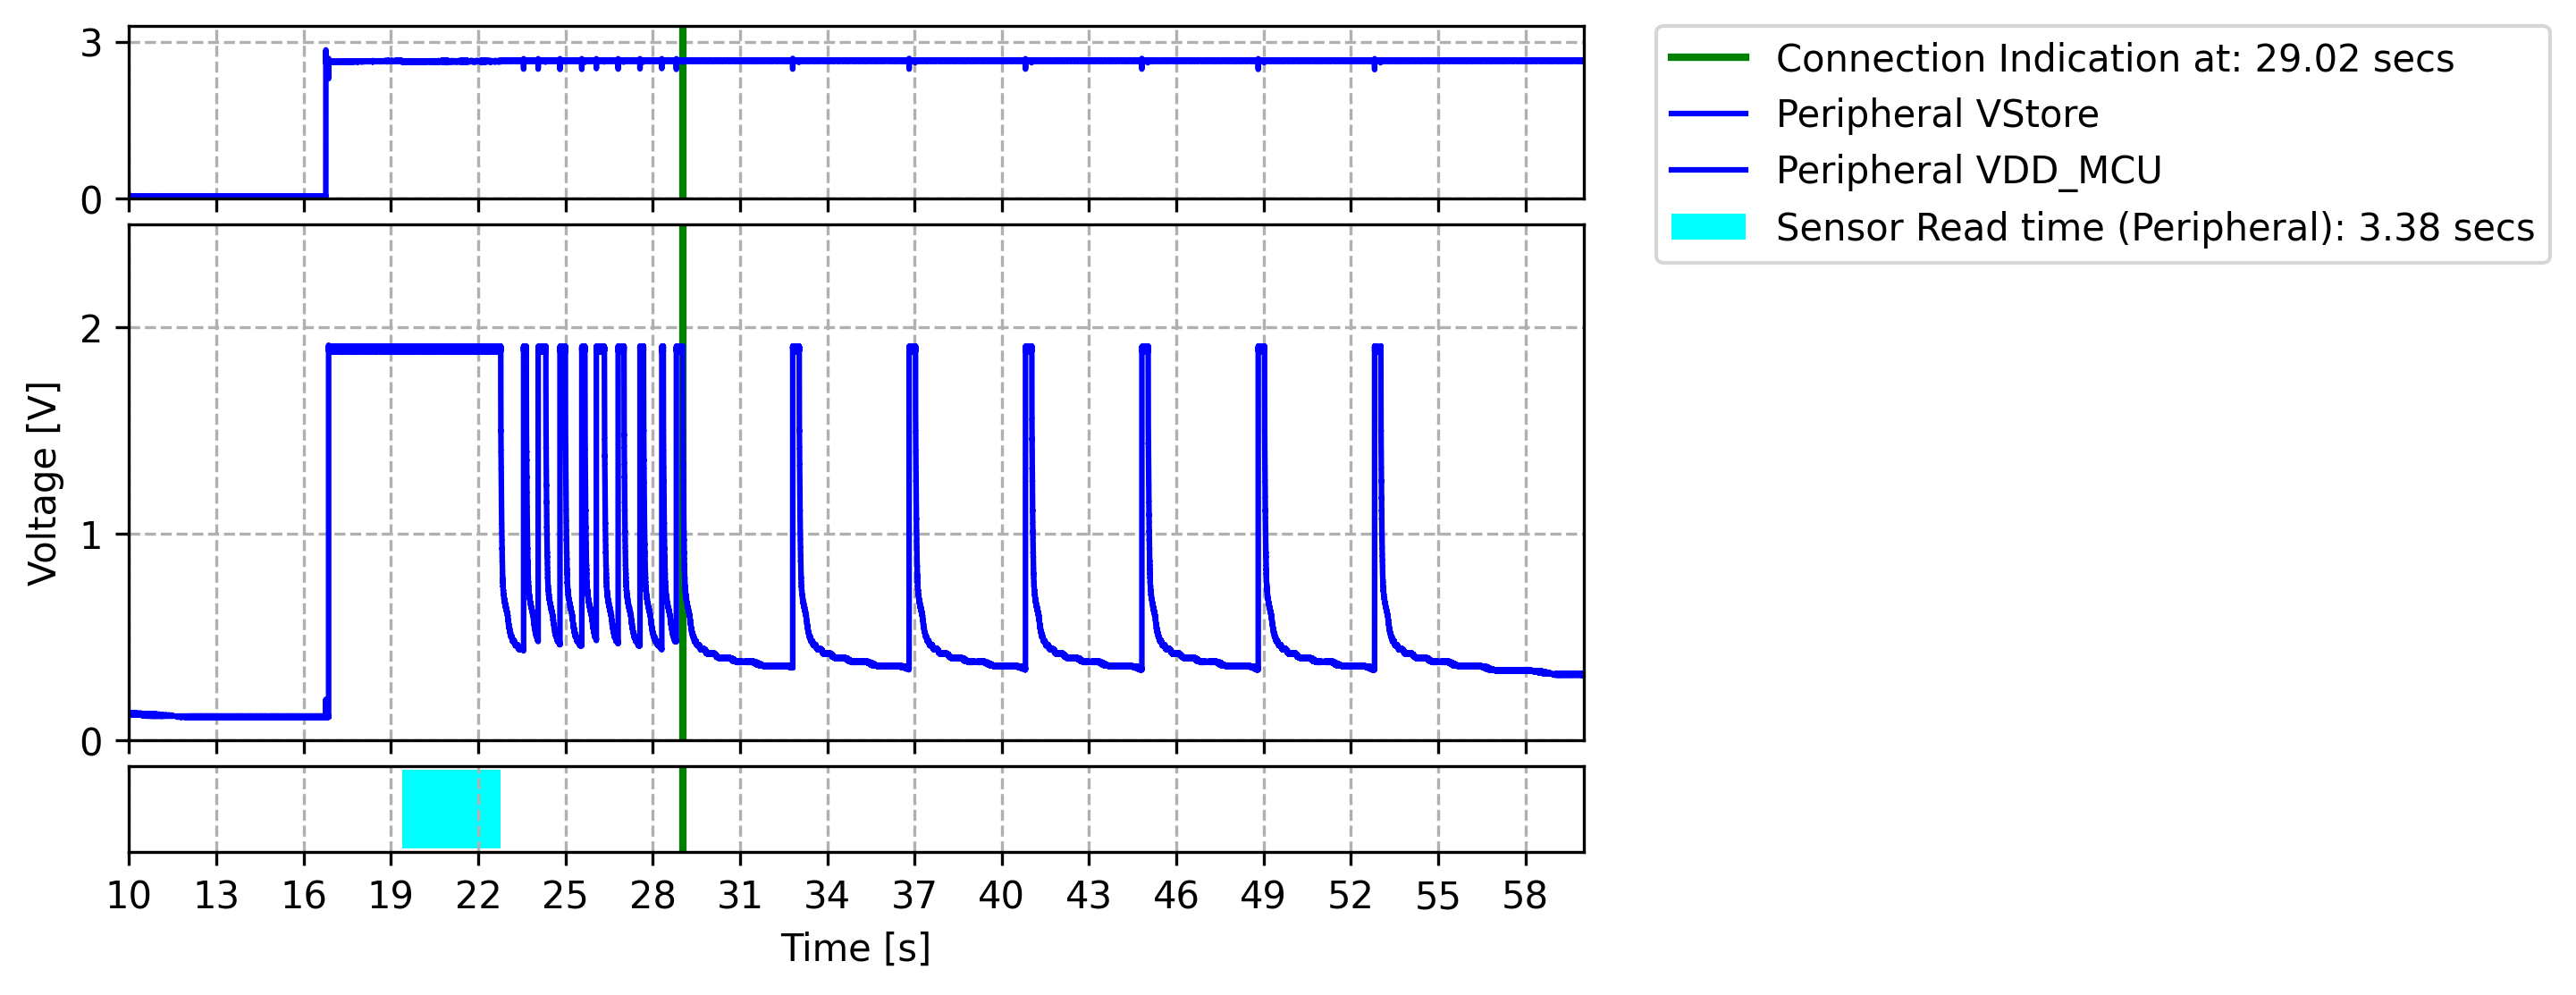
\includegraphics[width=1\linewidth]{chapters/Results/Connection_cardiosync_continous_peripheral.png}
        \caption{Voltage measurement for peripheral device.}
        \label{fig:continous_connection_cardiosync_peripheral}
        \vspace{1\baselineskip}
    \end{subfigure}
    \begin{subfigure}{1\linewidth}
        \centering
        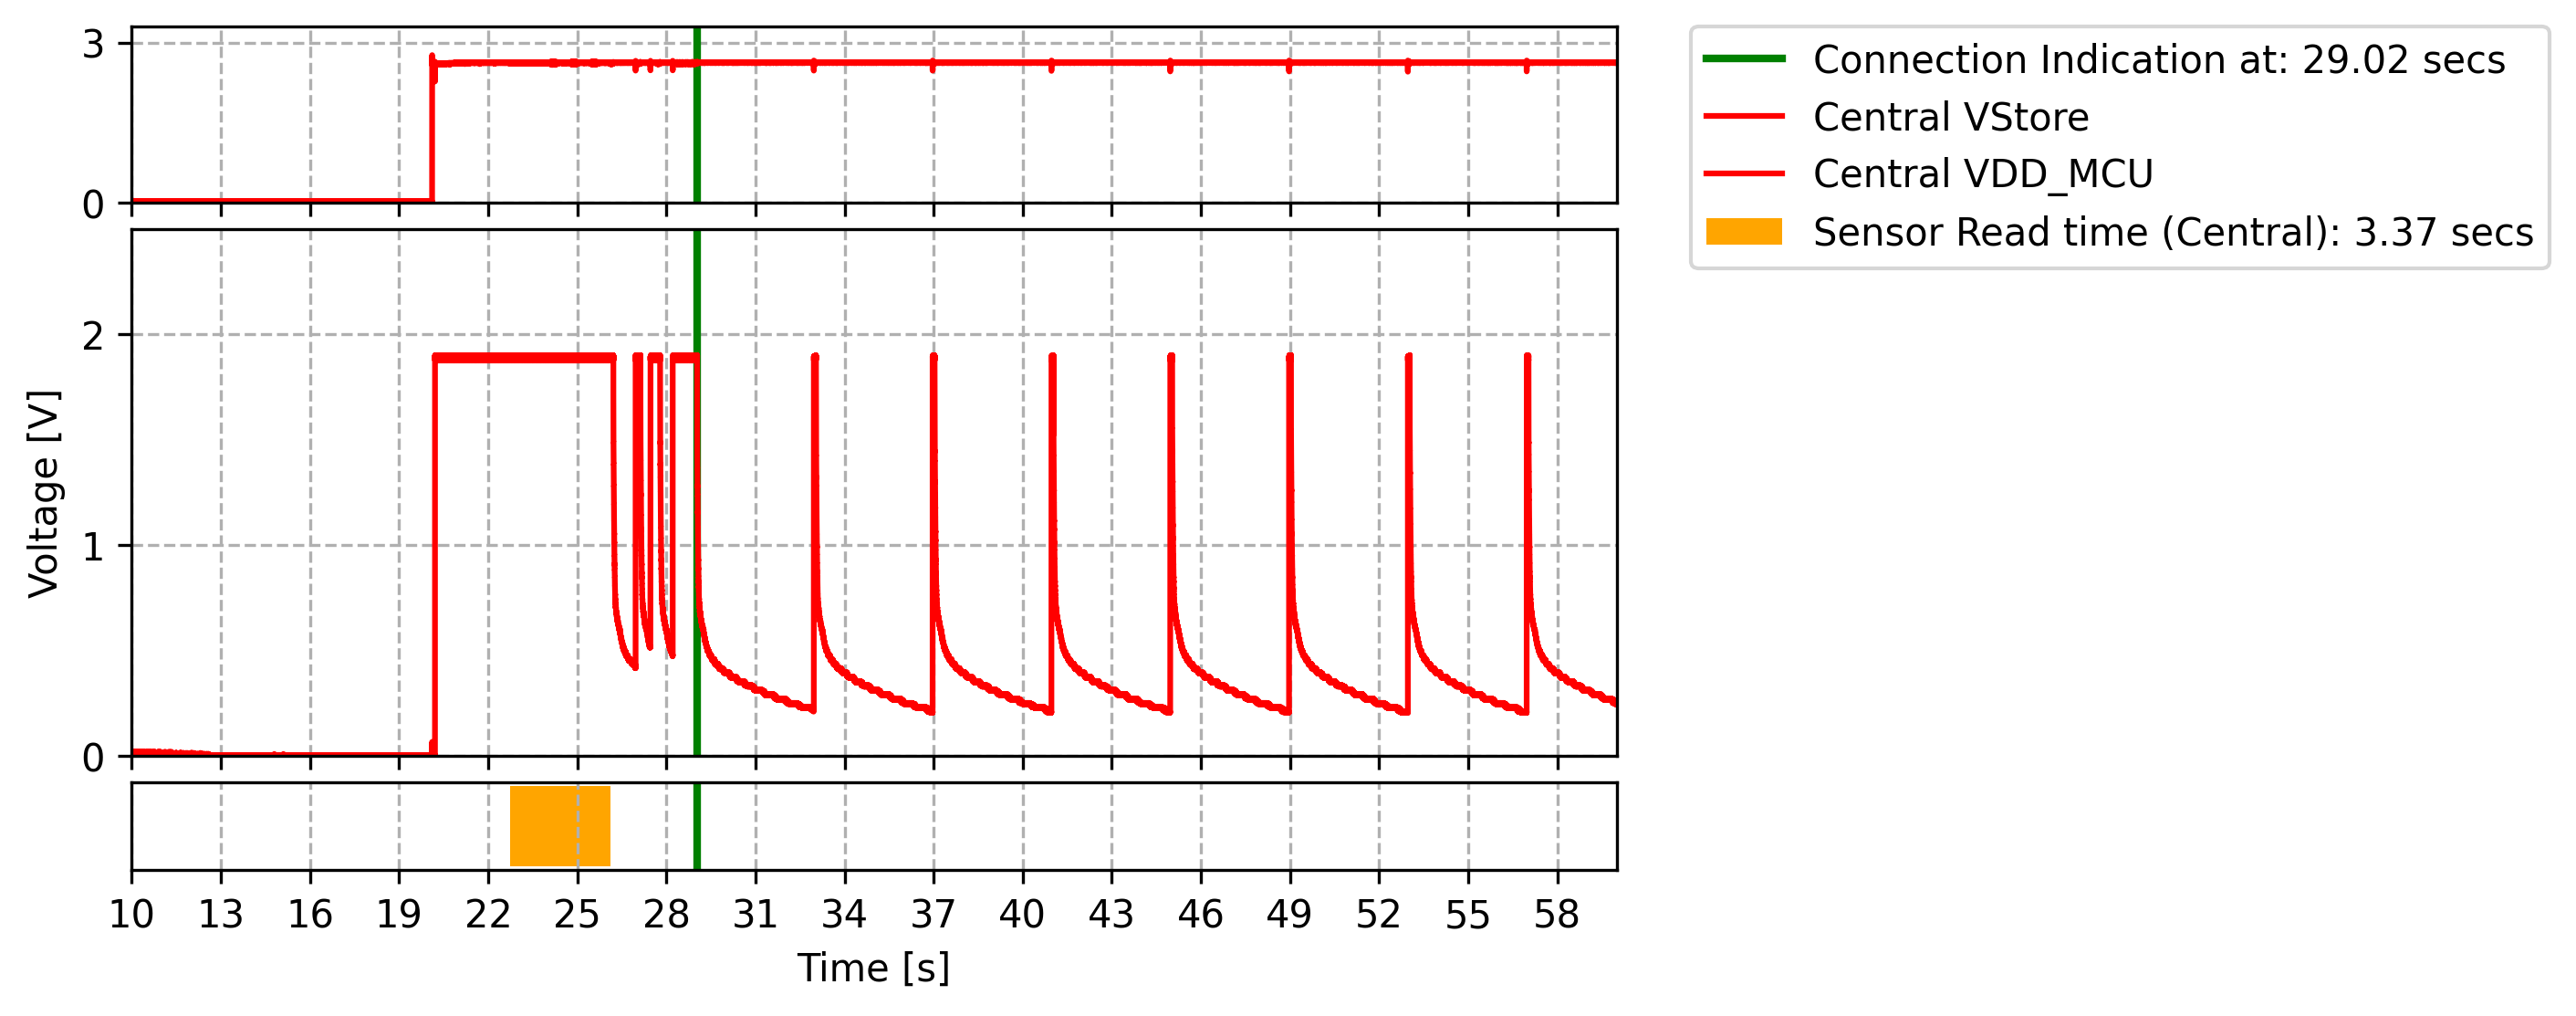
\includegraphics[width=1\linewidth]{chapters/Results/Connection_cardiosync_continous_central.png}
        \caption{Voltage measurement for central device.}
        \label{fig:continous_connection_cardiosync_central}
    \end{subfigure}
    \caption{Real-time voltage measurement for the CardioSync system \textit{with continuous power supply}. Each of the three plot in two devices shows different measurement. From the top to bottom in each device, 1) Plot of \(\text{V}_\text{Store}\) : Supply Voltage, 2) Plot of \(\text{V}_\text{DD\_MCU}\) : MCU voltage and 3) Plot of sensor read period indication. The green vertical line through all the plots indicates the successful BLE connection setup event.}
    \label{fig:continous_connection_cardiosync}
\end{figure}

\begin{figure}[ht]
    \begin{subfigure}{1\linewidth}
        \centering
        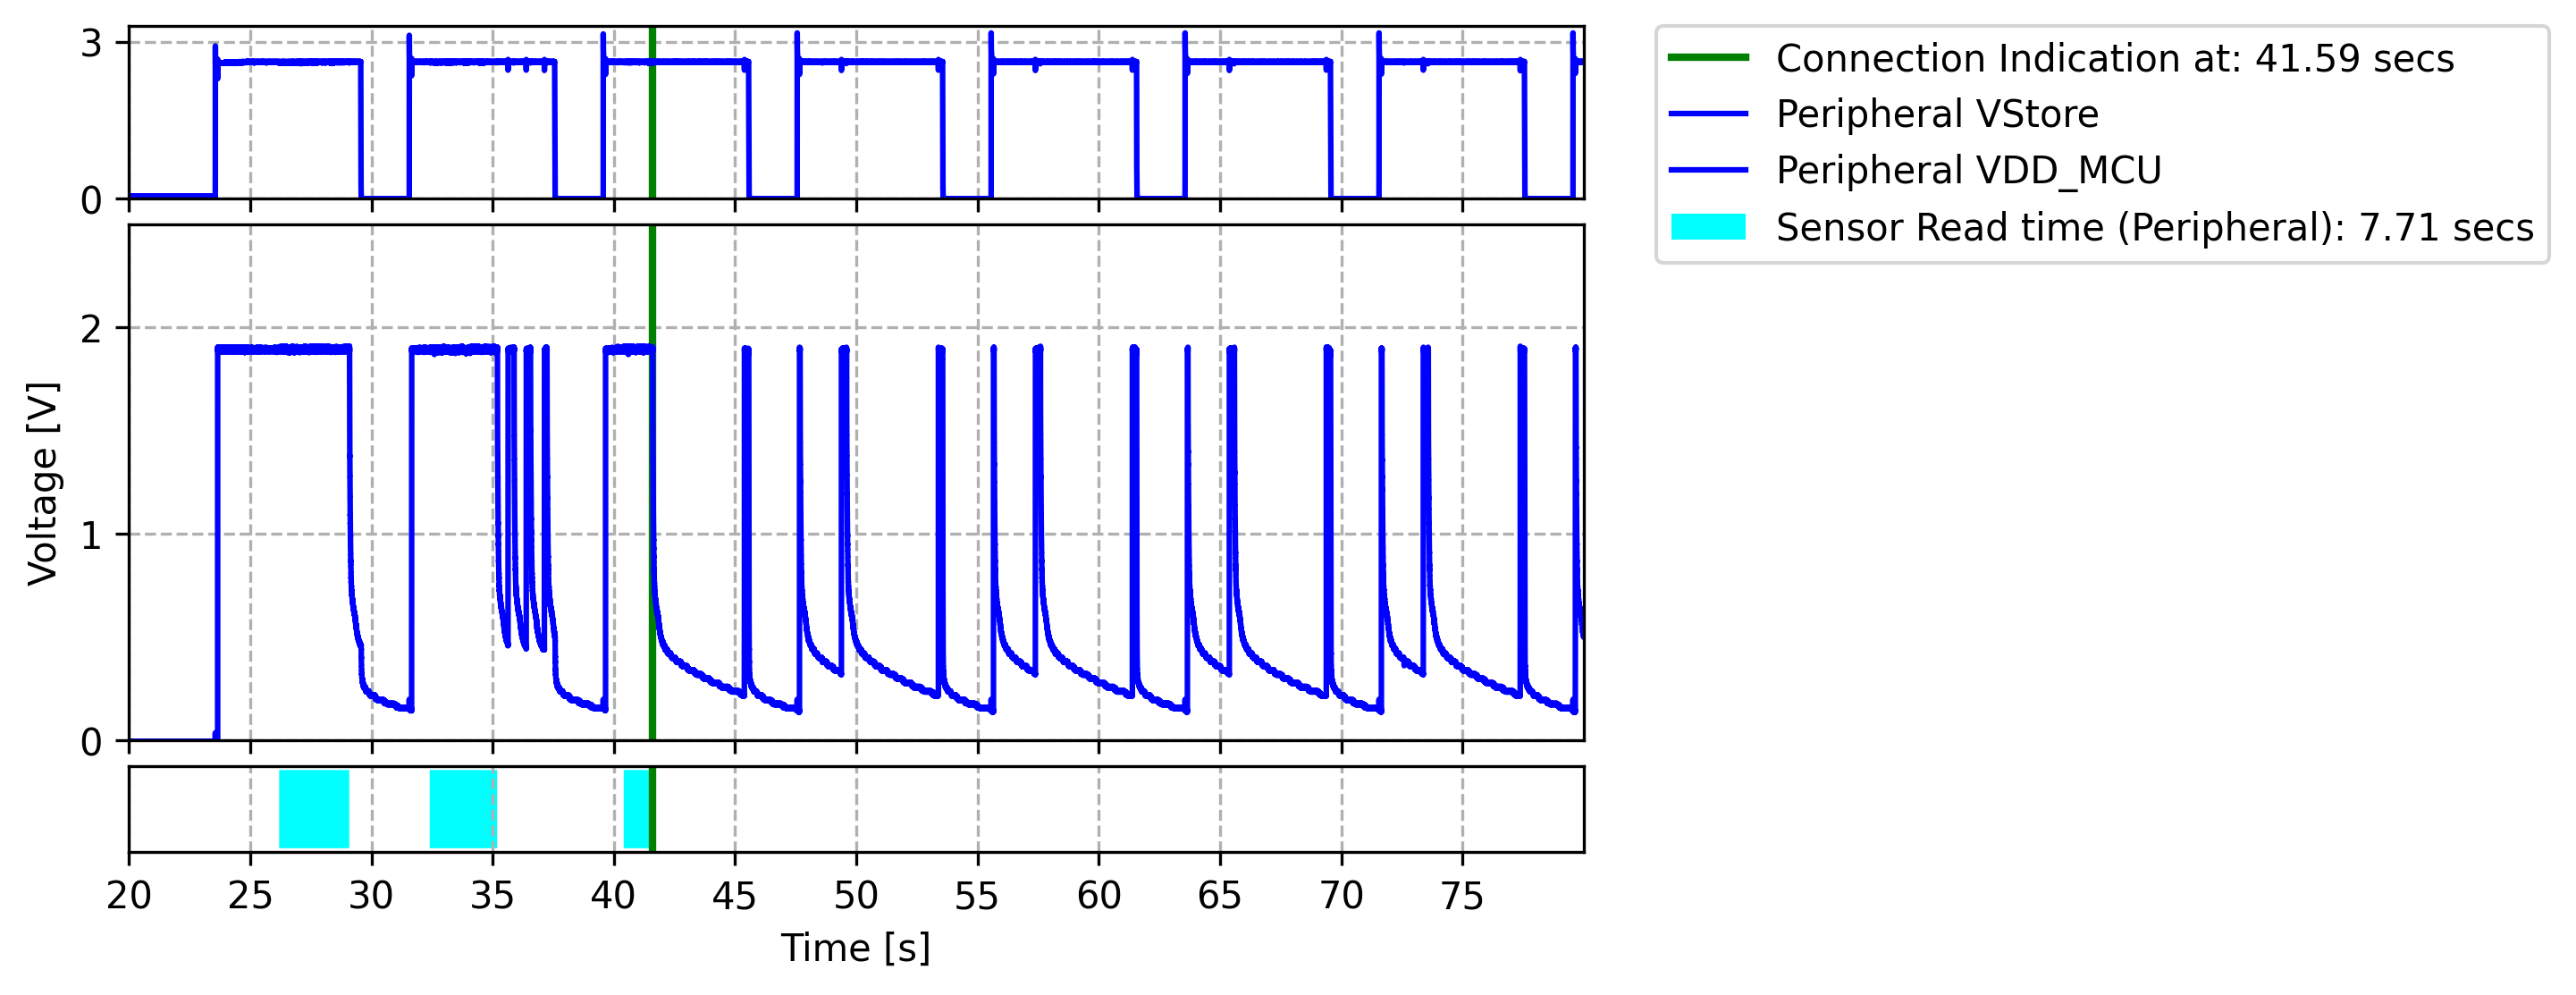
\includegraphics[width=1\linewidth]{chapters/Results/Connection_cardiosync_intermittent_peripheral.png}
        \caption{Voltage measurement for peripheral device.}
        \label{fig:intermittent_connection_cardiosync_peripheral}
        \vspace{1\baselineskip}
    \end{subfigure}
    \begin{subfigure}{1\linewidth}
        \centering
        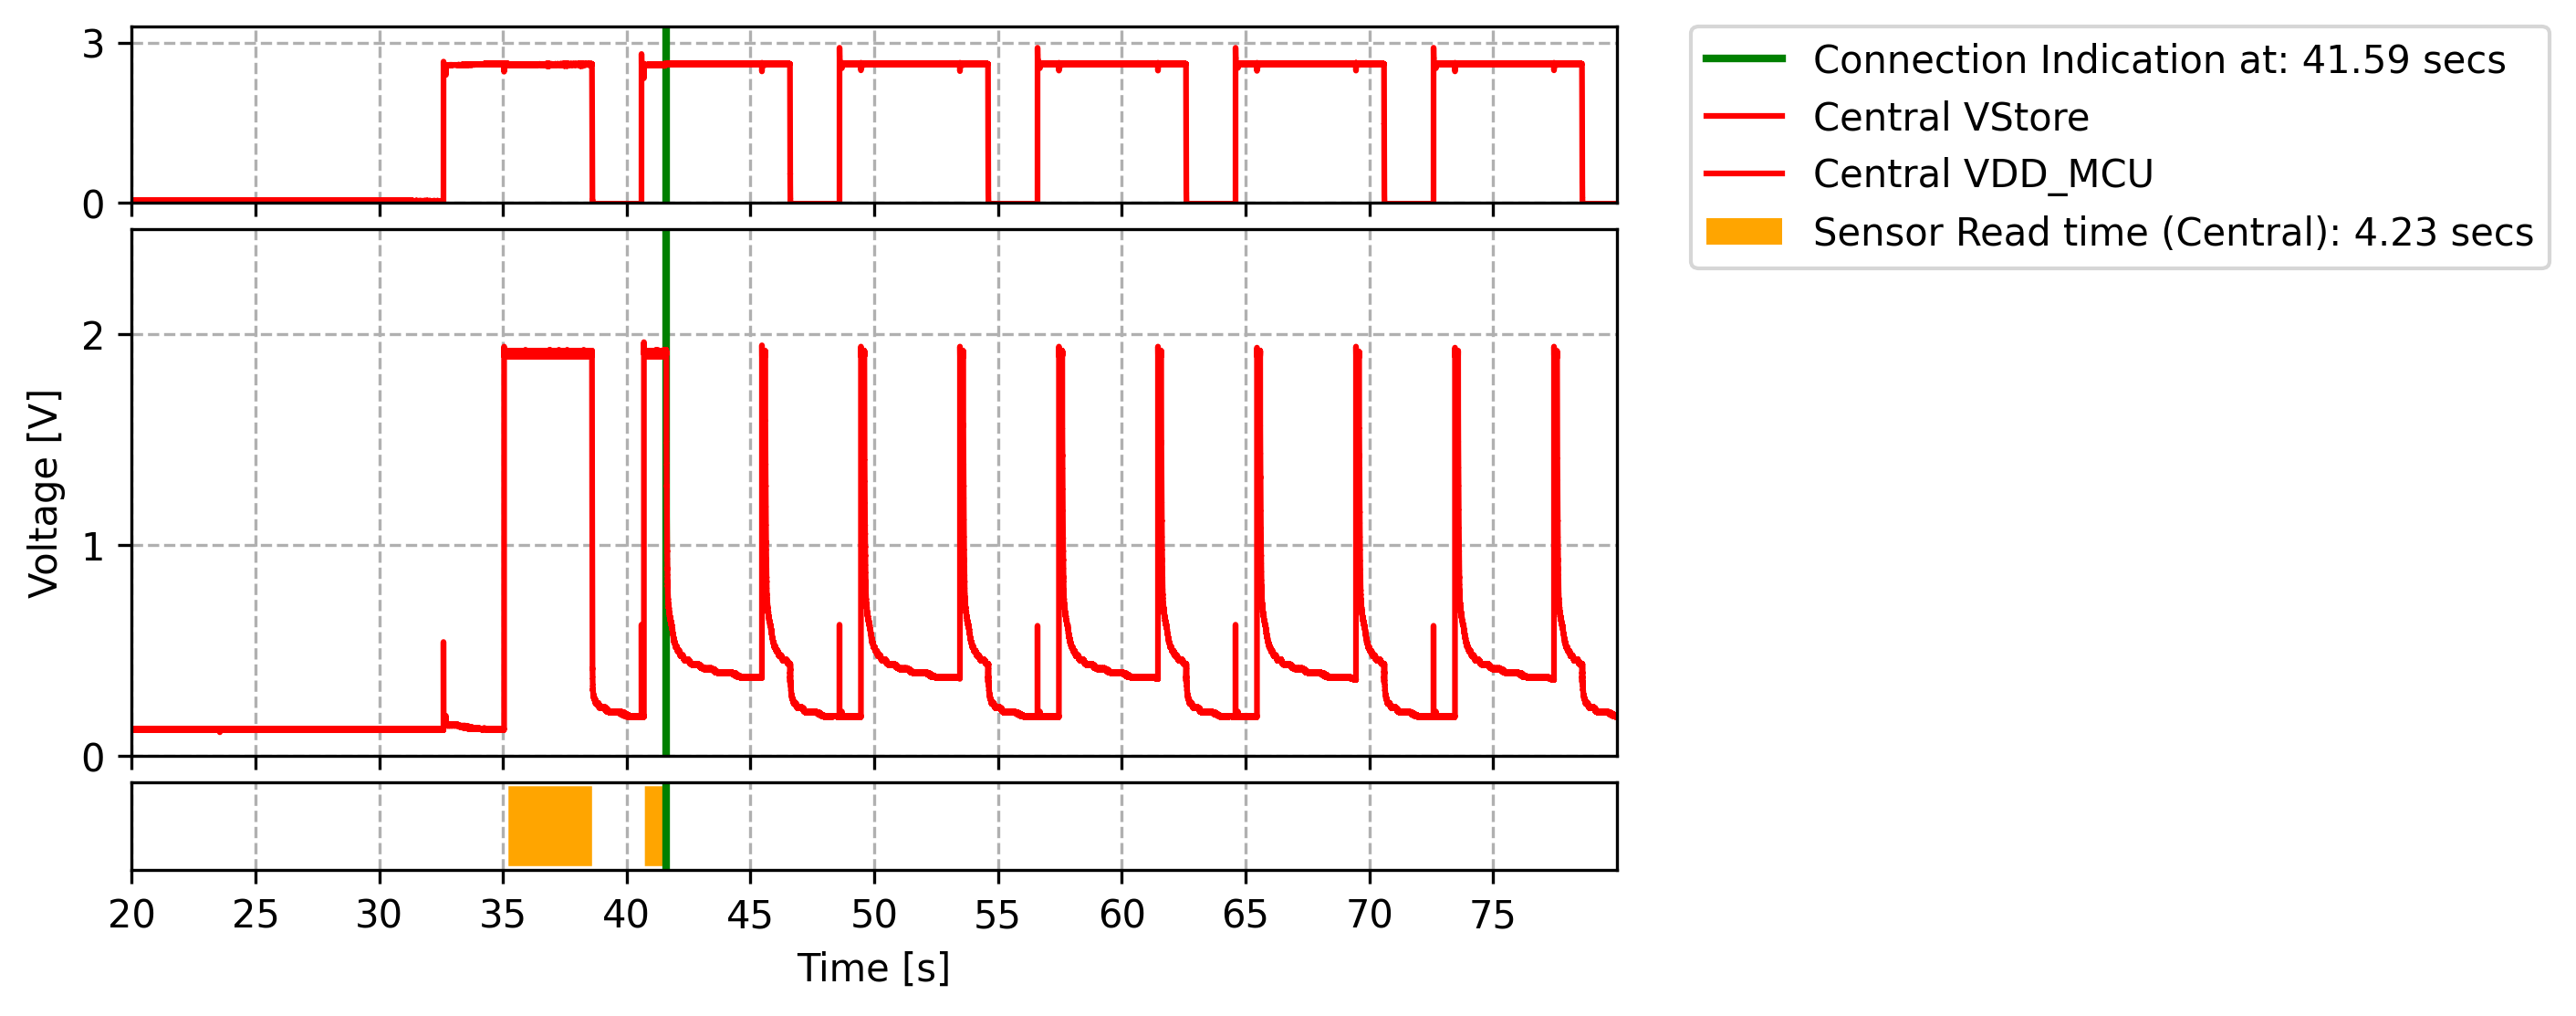
\includegraphics[width=1\linewidth]{chapters/Results/Connection_cardiosync_intermittent_central.png}
        \caption{Voltage measurement for central device.}
        \label{fig:intermittent_connection_cardiosync_central}
    \end{subfigure}
    \caption{Real-time voltage measurement for the CardioSync system \textit{with intermittent power supply}. Each of the three plot in two devices shows different measurement. From the top to bottom in each device, 1) Plot of \(\text{V}_\text{Store}\) : Supply Voltage, 2) Plot of \(\text{V}_\text{DD\_MCU}\) : MCU voltage and 3) Plot of sensor read period indication. The green vertical line through all the plots indicates the successful BLE connection setup event.}
    \label{fig:intermittent_connection_cardiosync}
\end{figure}

\begin{figure}[ht]
    \centering
    \begin{subfigure}{0.85\linewidth}        
        \centering
        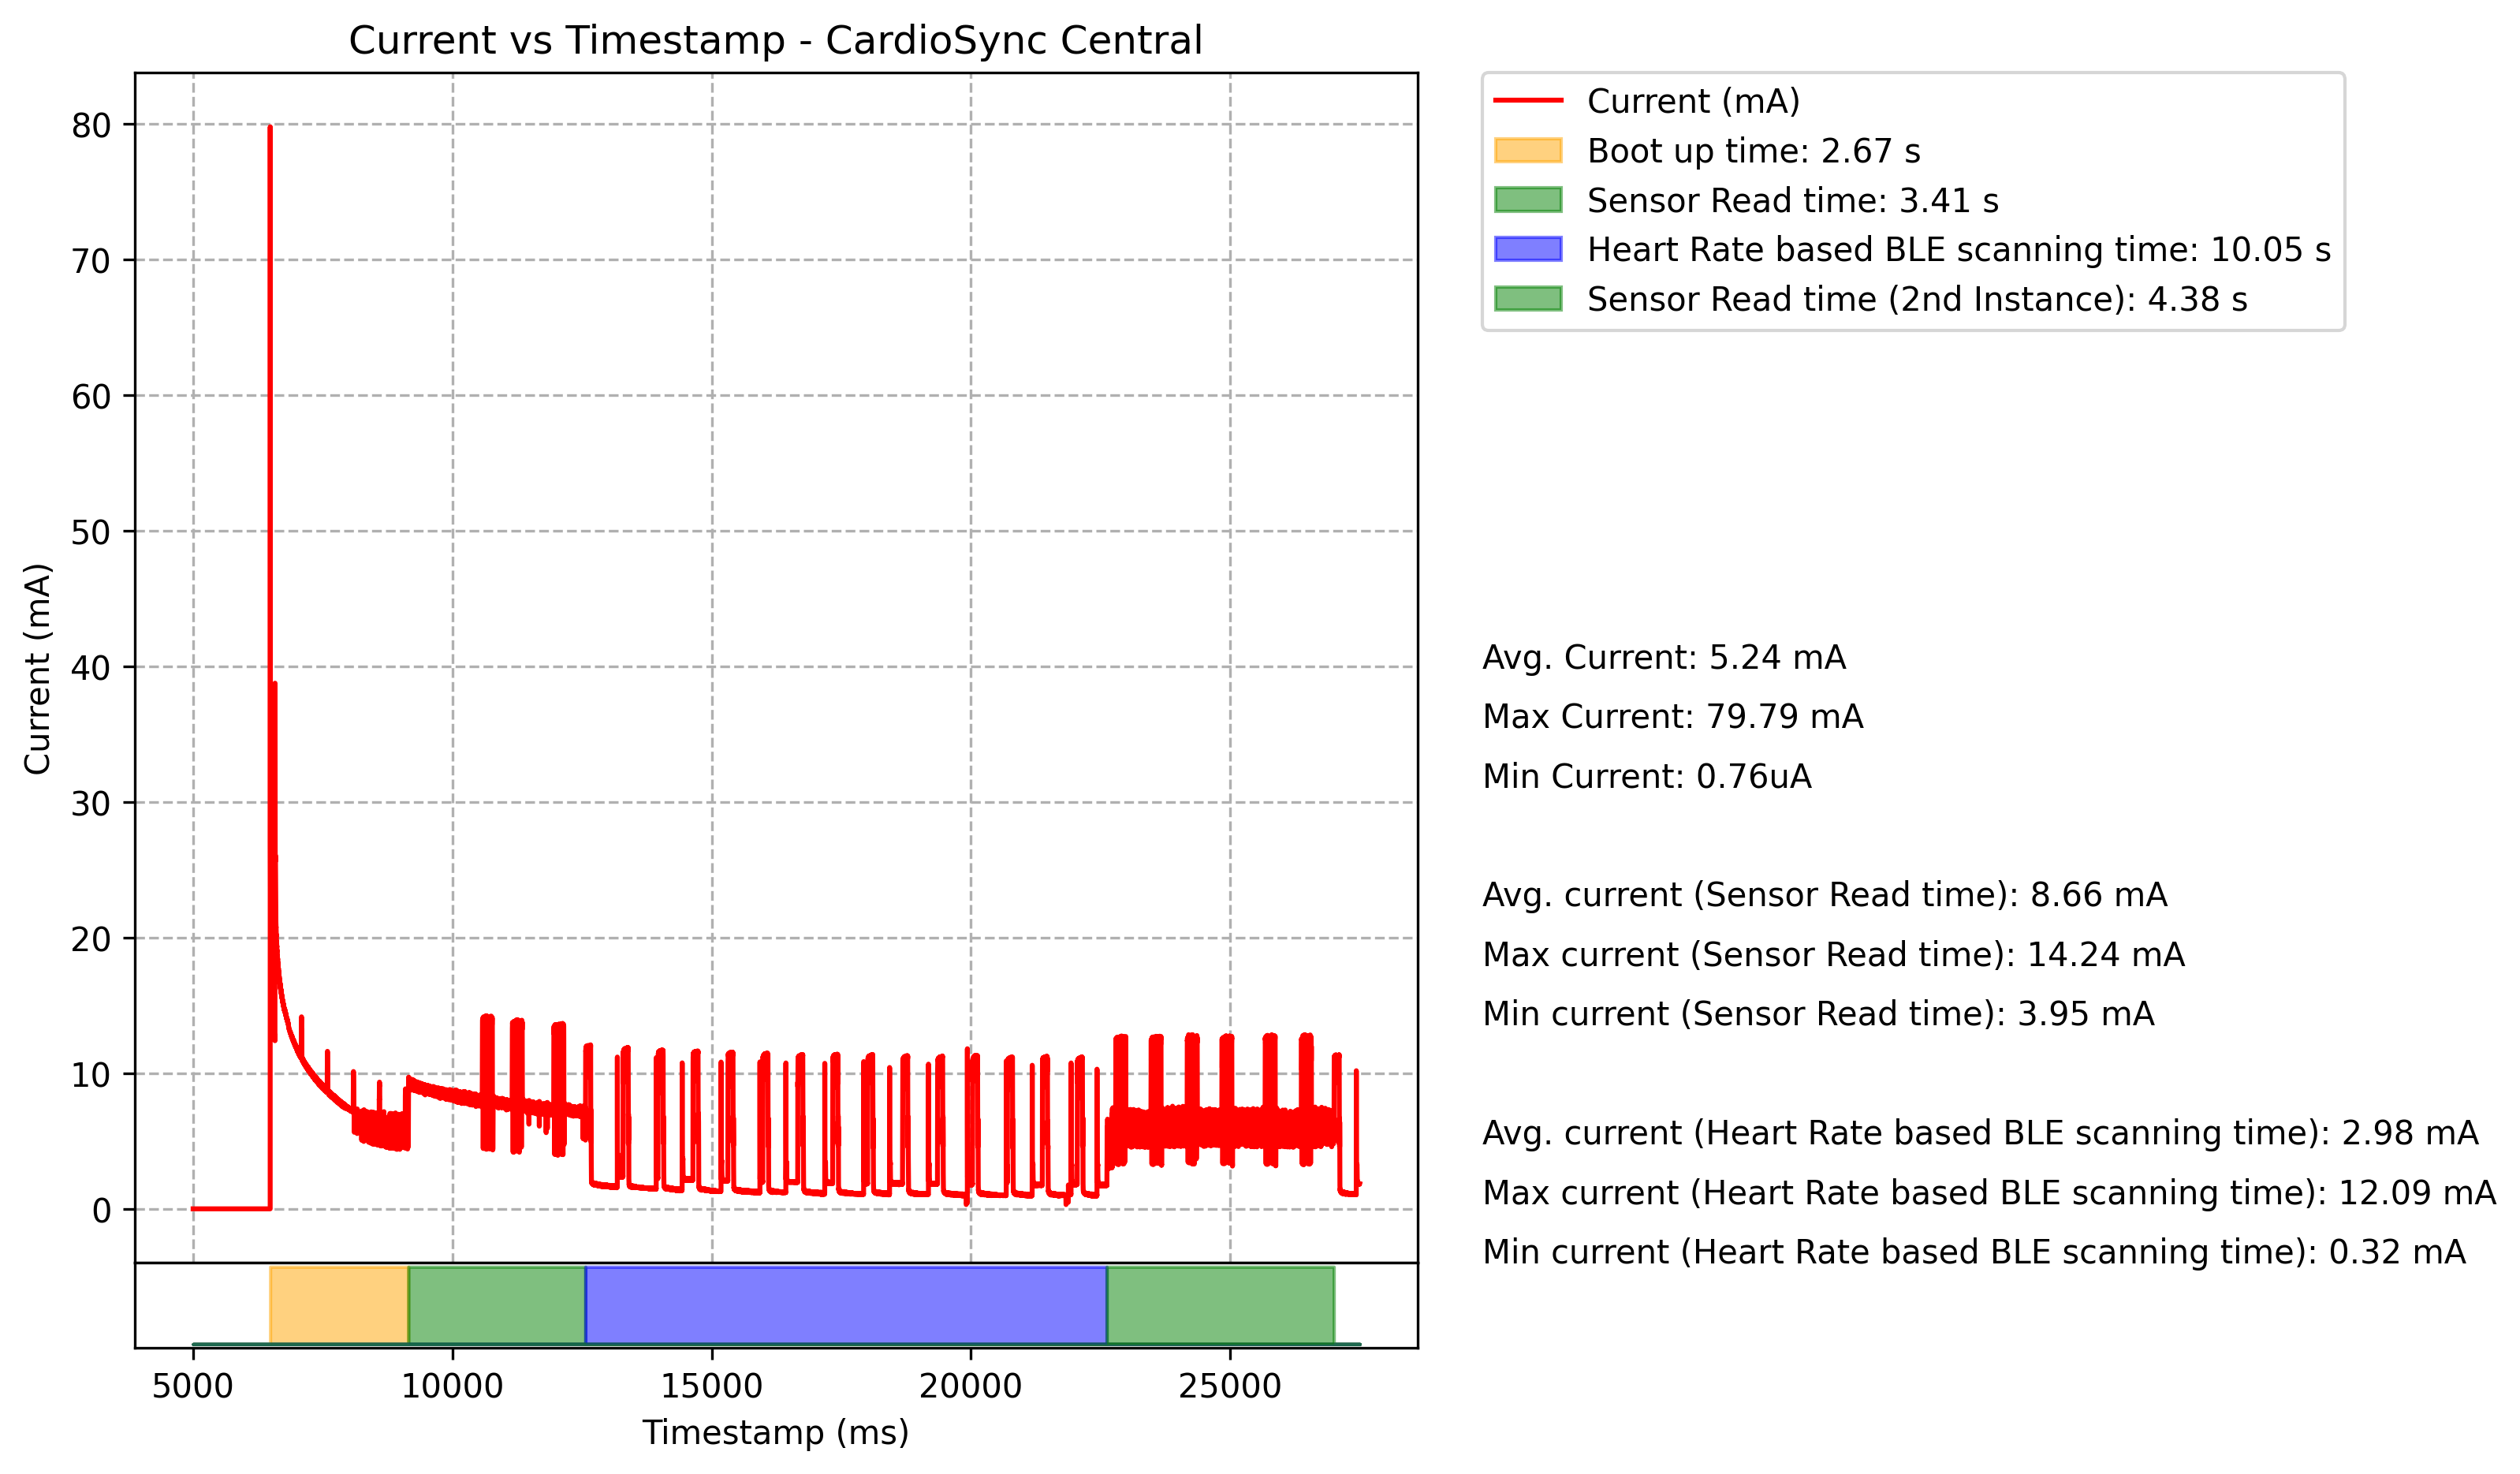
\includegraphics[width=\linewidth]{chapters/Results/Current vs Timestamp - CardioSync Central.png}
        \caption{Central}
        \label{fig:current_cardiosync_central}
    \end{subfigure}
    \begin{subfigure}{0.85\linewidth}    
        \centering
        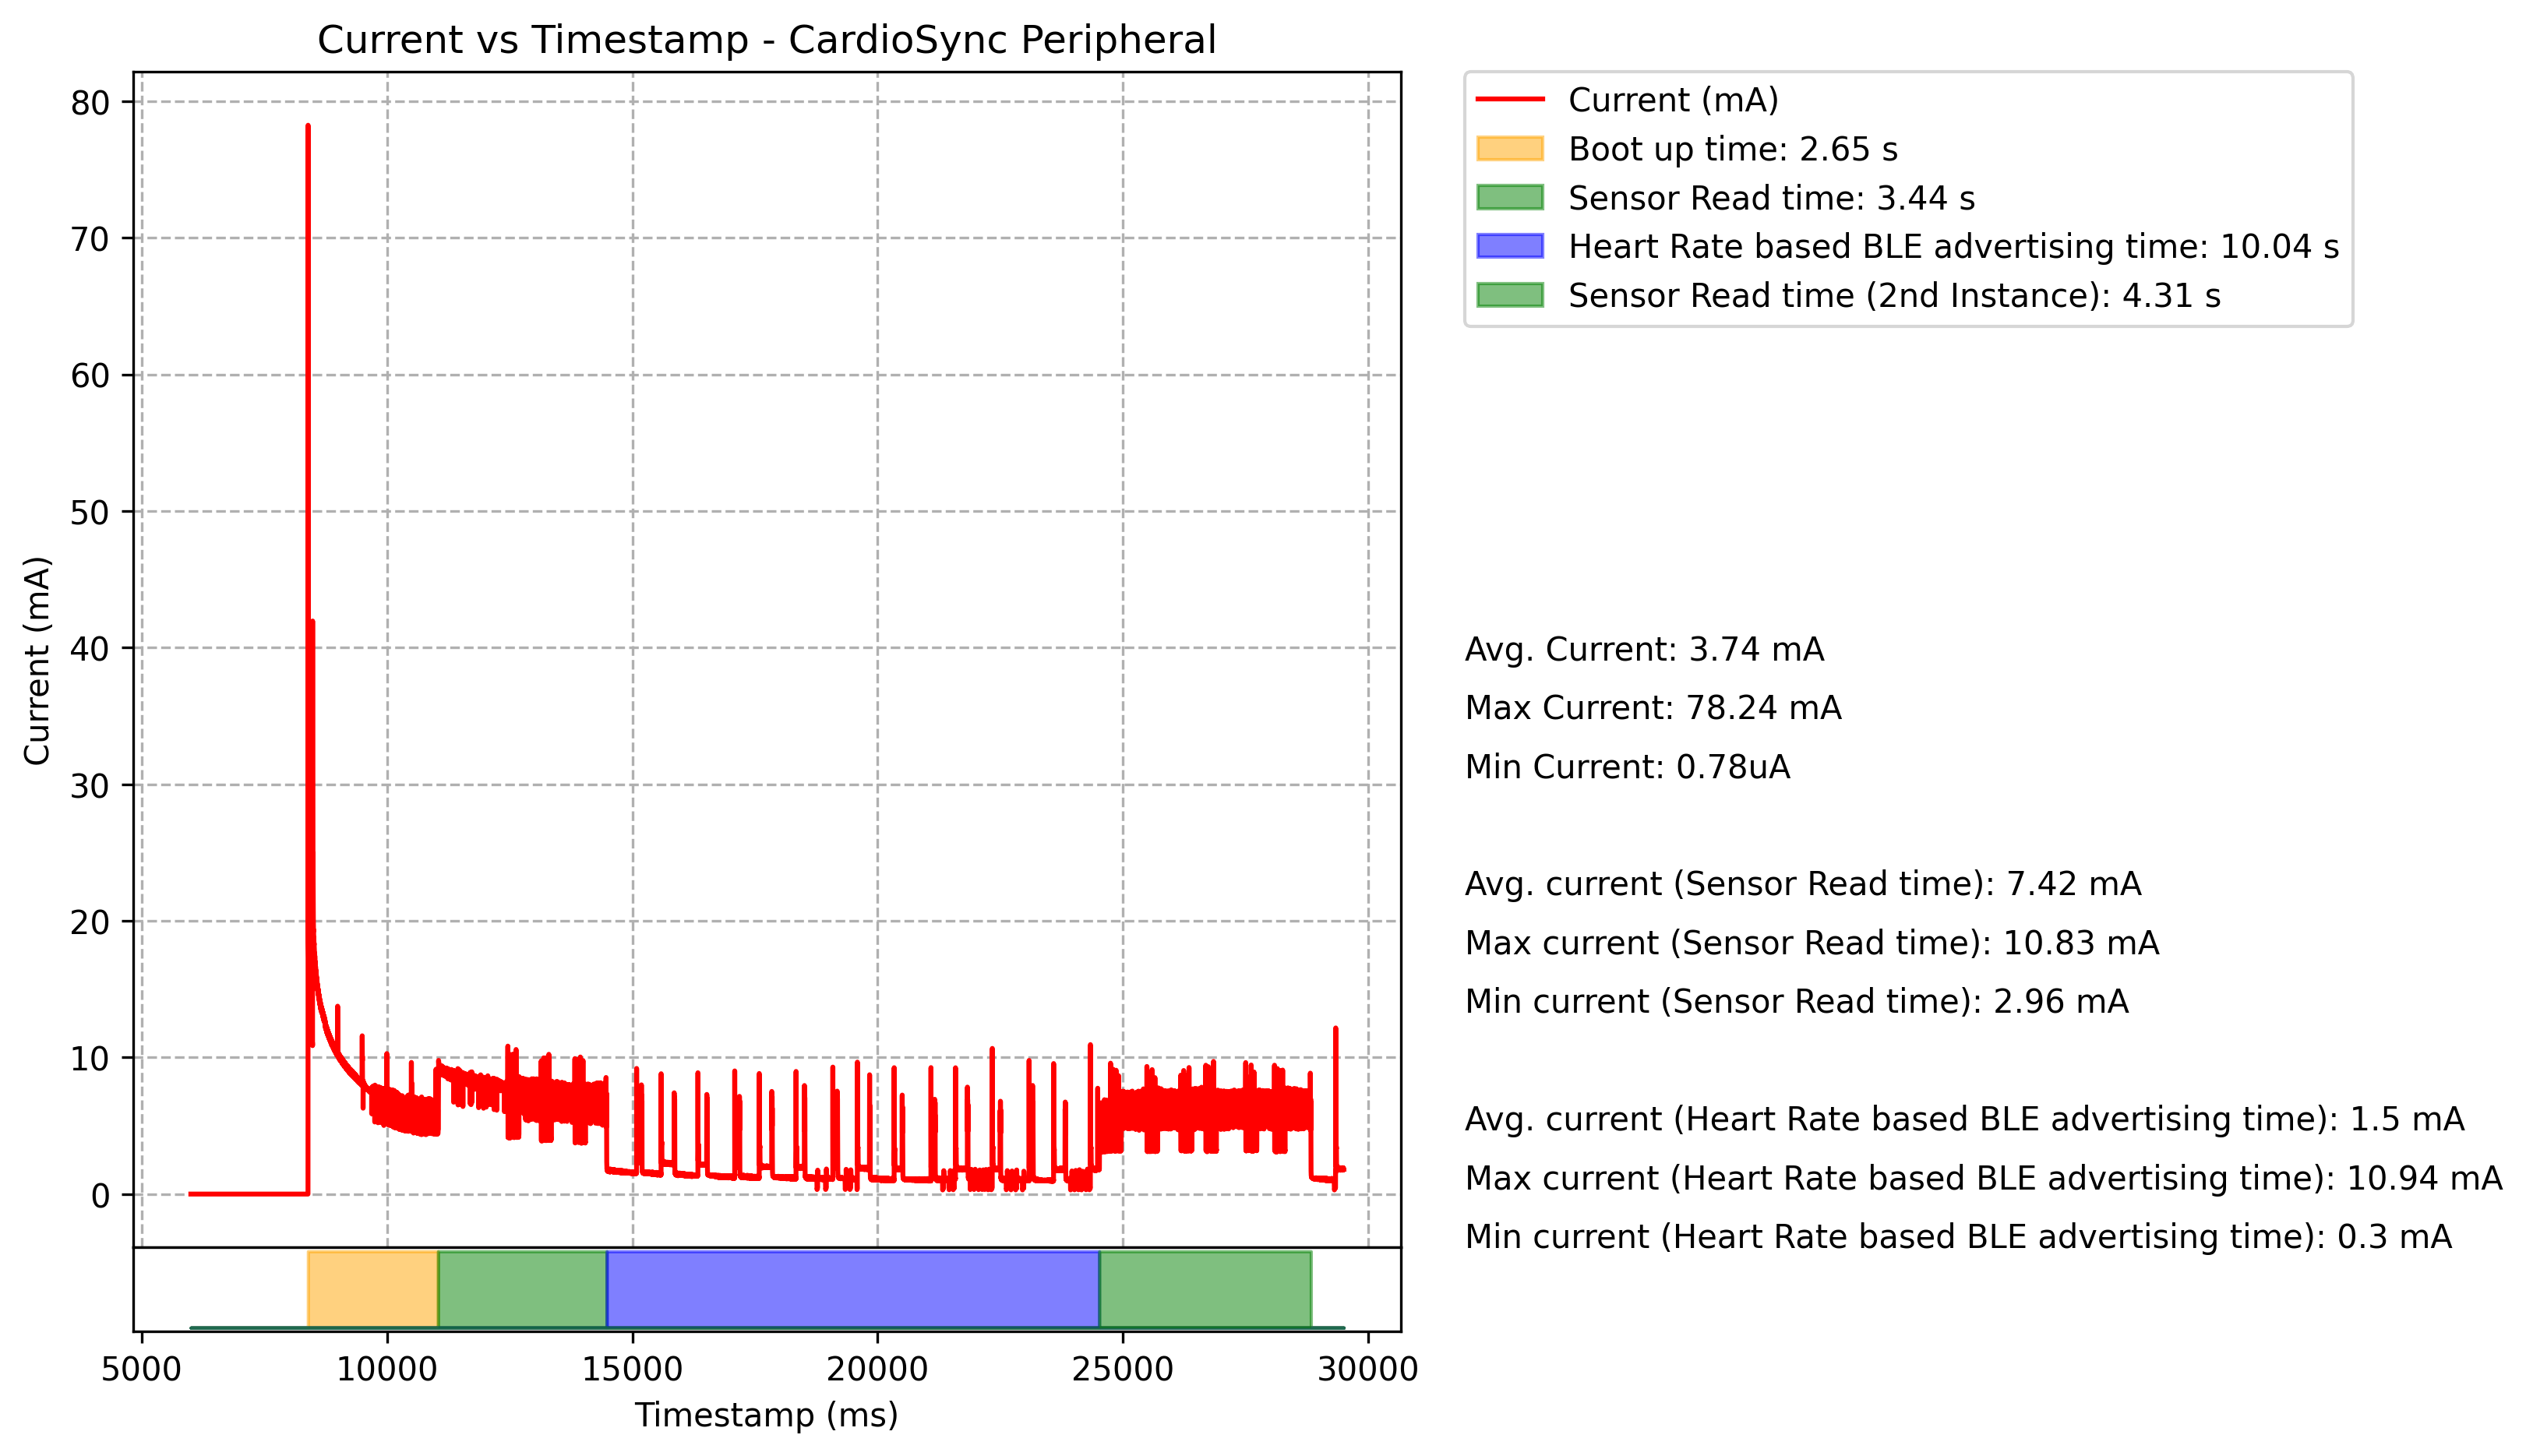
\includegraphics[width=\linewidth]{chapters/Results/Current vs Timestamp - CardioSync Peripheral.png}
        \caption{Peripheral}
        \label{fig:current_cardiosync_peripheral}
    \end{subfigure}
    \caption{Current measurement in idle state without connection establishment for CardioSync systems. Average current consumed in real-time during different phases of the system are differentiated with different colours.}
    \label{fig:current_cardiosync}
\end{figure}

\subsubsection{Validation of Working CardioSync}
The time series plot depicted in \autoref{fig:continous_connection_cardiosync} illustrates the operation of CardioSync framework with continuous powered input. It can be asserted from the plot that there is the periodic shutdown of \(\text{V}_\text{DD\_MCU}\) during times of inactivity, therefore corroborating the anticipated power-saving benefits associated with the integration of FreeBie.
\vspace{1\baselineskip}

\noindent As elucidated in Chapter \ref{chap:implementation}, the system from \autoref{fig:continous_connection_cardiosync} demonstrates the anticipated functionality of "Read and Synchronise" for a period of \textit{3.40 seconds} where the sensor is being actively read. Followed by that, we also see  the "Sleep and Synchronise" functionality, where the system exclusively reactivates at the interval of each heartbeat pulse in order to initiate a connection. The connection establishment event, which is closely synced with the heart rate pulses, is shown by the green vertical line in Figure \ref{fig:continous_connection_cardiosync}.
\vspace{1\baselineskip}

\noindent A similar verification was conducted under intermittent power supply using a square wave signal with a duty cycle of 75\% for a duration of 8 seconds. The time series plot (\autoref{fig:intermittent_connection_cardiosync}) reveals the system's adaptability to changing power availability, as connections continue to be established in coordination with the heart beat, despite power fluctuations. In addition, the CardioSync system was tested across various square wave periods with different duty cycles as shown in Table \ref{tab:cardiosync_intermittent_exp} in Appendix \ref{app:appendix_a}, demonstrating its adaptability to different supply configurations.

\subsubsection{Current Measurement of CardioSync system}
Figure \ref{fig:current_cardiosync}, gives us the current measurement for different phases of the CardioSync system operation for synchronising BLE connection. The measured current values are afterwards utilised for comparative analysis against naive reference system.
\vspace{1\baselineskip}

\noindent It is important to note that the "Read and Synchronise" phase requires a higher current compared to the "Sleep and Synchronise" phase. This behaviour is substantiated across both central and peripheral devices in the current measurement-driven evaluation. In the Central device, "Read and Synchronise" phase happens for around \textit{3.41 seconds} and consumes an average current of approximately \textit{8.66mA}. Similarly, the Peripheral device registers \textit{7.42mA} over a \textit{3.44-second} interval of sensor read phase. Notably, during the "Sleep and Synchronise" phase of 10 seconds, both central and peripheral devices exhibit a substantially lower average current consumption—\textit{2.98mA and 1.5mA}, respectively.
\vspace{1\baselineskip}

\noindent The values of these evaluation are afterwards utilised in the computation of the energy expended by the device for the purpose of synchronising a BLE connection.


\section{Comparative Analysis against Naive Reference Design}
In this section, we start by introducing a naive reference model of Battery-Free BLE. This model will be used as a yardstick to gauge the effectiveness of our synchronised CardioSync system.

\subsection{Naive Reference FreeBie Model}

\noindent To ensure a comprehensive comparison, the reference system used is the FreeBie system, which lacks any synchronisation method. For experimental purposes, both the Central and Peripheral components of the FreeBie reference model were intentionally set to have matching Advertising and Scanning intervals, preventing any permanent link failure.
\vspace{1\baselineskip}

\begin{table}[t]
\centering
\begin{tabular}{|c|cc|}
\hline
\textbf{\begin{tabular}[c]{@{}c@{}}Configuration\\ Name\end{tabular}} & \multicolumn{2}{c|}{\textbf{\begin{tabular}[c]{@{}c@{}}Configured BLE\\ parameters\end{tabular}}} \\ \hline
\cellcolor[HTML]{32CB00} & \multicolumn{1}{c|}{\textit{\begin{tabular}[c]{@{}c@{}}Advertising\\ Interval\end{tabular}}} & 6 seconds        \\ \cline{2-3} 
\cellcolor[HTML]{32CB00} & \multicolumn{1}{c|}{\textit{\begin{tabular}[c]{@{}c@{}}Scanning\\ Interval\end{tabular}}}    & 6 seconds        \\ \cline{2-3} 
\multirow{-3}{*}{\cellcolor[HTML]{32CB00}\textbf{Low}}    & \multicolumn{1}{c|}{\textit{\begin{tabular}[c]{@{}c@{}}Scanning\\ Window\end{tabular}}} & 1 second         \\ \hline
\cellcolor[HTML]{FFCB2F} & \multicolumn{1}{c|}{\textit{\begin{tabular}[c]{@{}c@{}}Advertising\\ Interval\end{tabular}}} & 2 seconds        \\ \cline{2-3} 
\cellcolor[HTML]{FFCB2F} & \multicolumn{1}{c|}{\textit{\begin{tabular}[c]{@{}c@{}}Scanning\\ Interval\end{tabular}}}    & 2 seconds        \\ \cline{2-3} 
\multirow{-3}{*}{\cellcolor[HTML]{FFCB2F}\textbf{Medium}} & \multicolumn{1}{c|}{\textit{\begin{tabular}[c]{@{}c@{}}Scanning\\ Window\end{tabular}}} & 500 milliseconds \\ \hline
\cellcolor[HTML]{FD6864} & \multicolumn{1}{c|}{\textit{\begin{tabular}[c]{@{}c@{}}Advertising\\ Interval\end{tabular}}} & 500 milliseconds \\ \cline{2-3} 
\cellcolor[HTML]{FD6864} & \multicolumn{1}{c|}{\textit{\begin{tabular}[c]{@{}c@{}}Scanning\\ Interval\end{tabular}}}    & 500 milliseconds \\ \cline{2-3} 
\multirow{-3}{*}{\cellcolor[HTML]{FD6864}\textbf{High}}  & \multicolumn{1}{c|}{\textit{\begin{tabular}[c]{@{}c@{}}Scanning\\ Window\end{tabular}}} & 125 milliseconds \\ \hline
\end{tabular}
\caption{Chosen BLE parameters for Reference FreeBie system}
\label{tab:ble_params_freebie}
\end{table}

\noindent To enrich our data pool, we selected three distinct BLE configurations for the FreeBie system, each characterised by varying energy consumption, as detailed in \autoref{tab:ble_params_freebie}. To provide practical real-world context, each configuration represents a scenario within the realm of body sensor networks. These diverse scenarios provide a practical basis for comparing the performance of the CardioSync framework with the reference FreeBie system.

\begin{itemize}
    \item \textbf{FreeBie Low (Limited-Energy Scenario):} This scenario envisions a wearable sensor attached to a person's shoe sole, relying on minimal energy generated through piezoelectric energy harvesting from each step. In this challenging environment, efficient energy management during connection attempts is crucial.
    
    \item \textbf{FreeBie Medium (Balanced-Energy Scenario):} In this scenario, the device is part of a fitness tracker, like a wristband, accessing moderate energy from a solar cells. While energy constraints are less severe than in the Low scenario, efficient energy use remains vital.
    
    \item \textbf{FreeBie High (Abundant-Energy Scenario):} Two energy sources are considered, one on the wrist and one on the ankle, harnessing abundant energy from solar cells and motion harvesting, respectively. These devices can expend energy liberally for frequent connection attempts, emphasising connection efficiency.
\end{itemize}


\begin{figure}[t]
    \begin{subfigure}{0.5\linewidth}
        \centering
        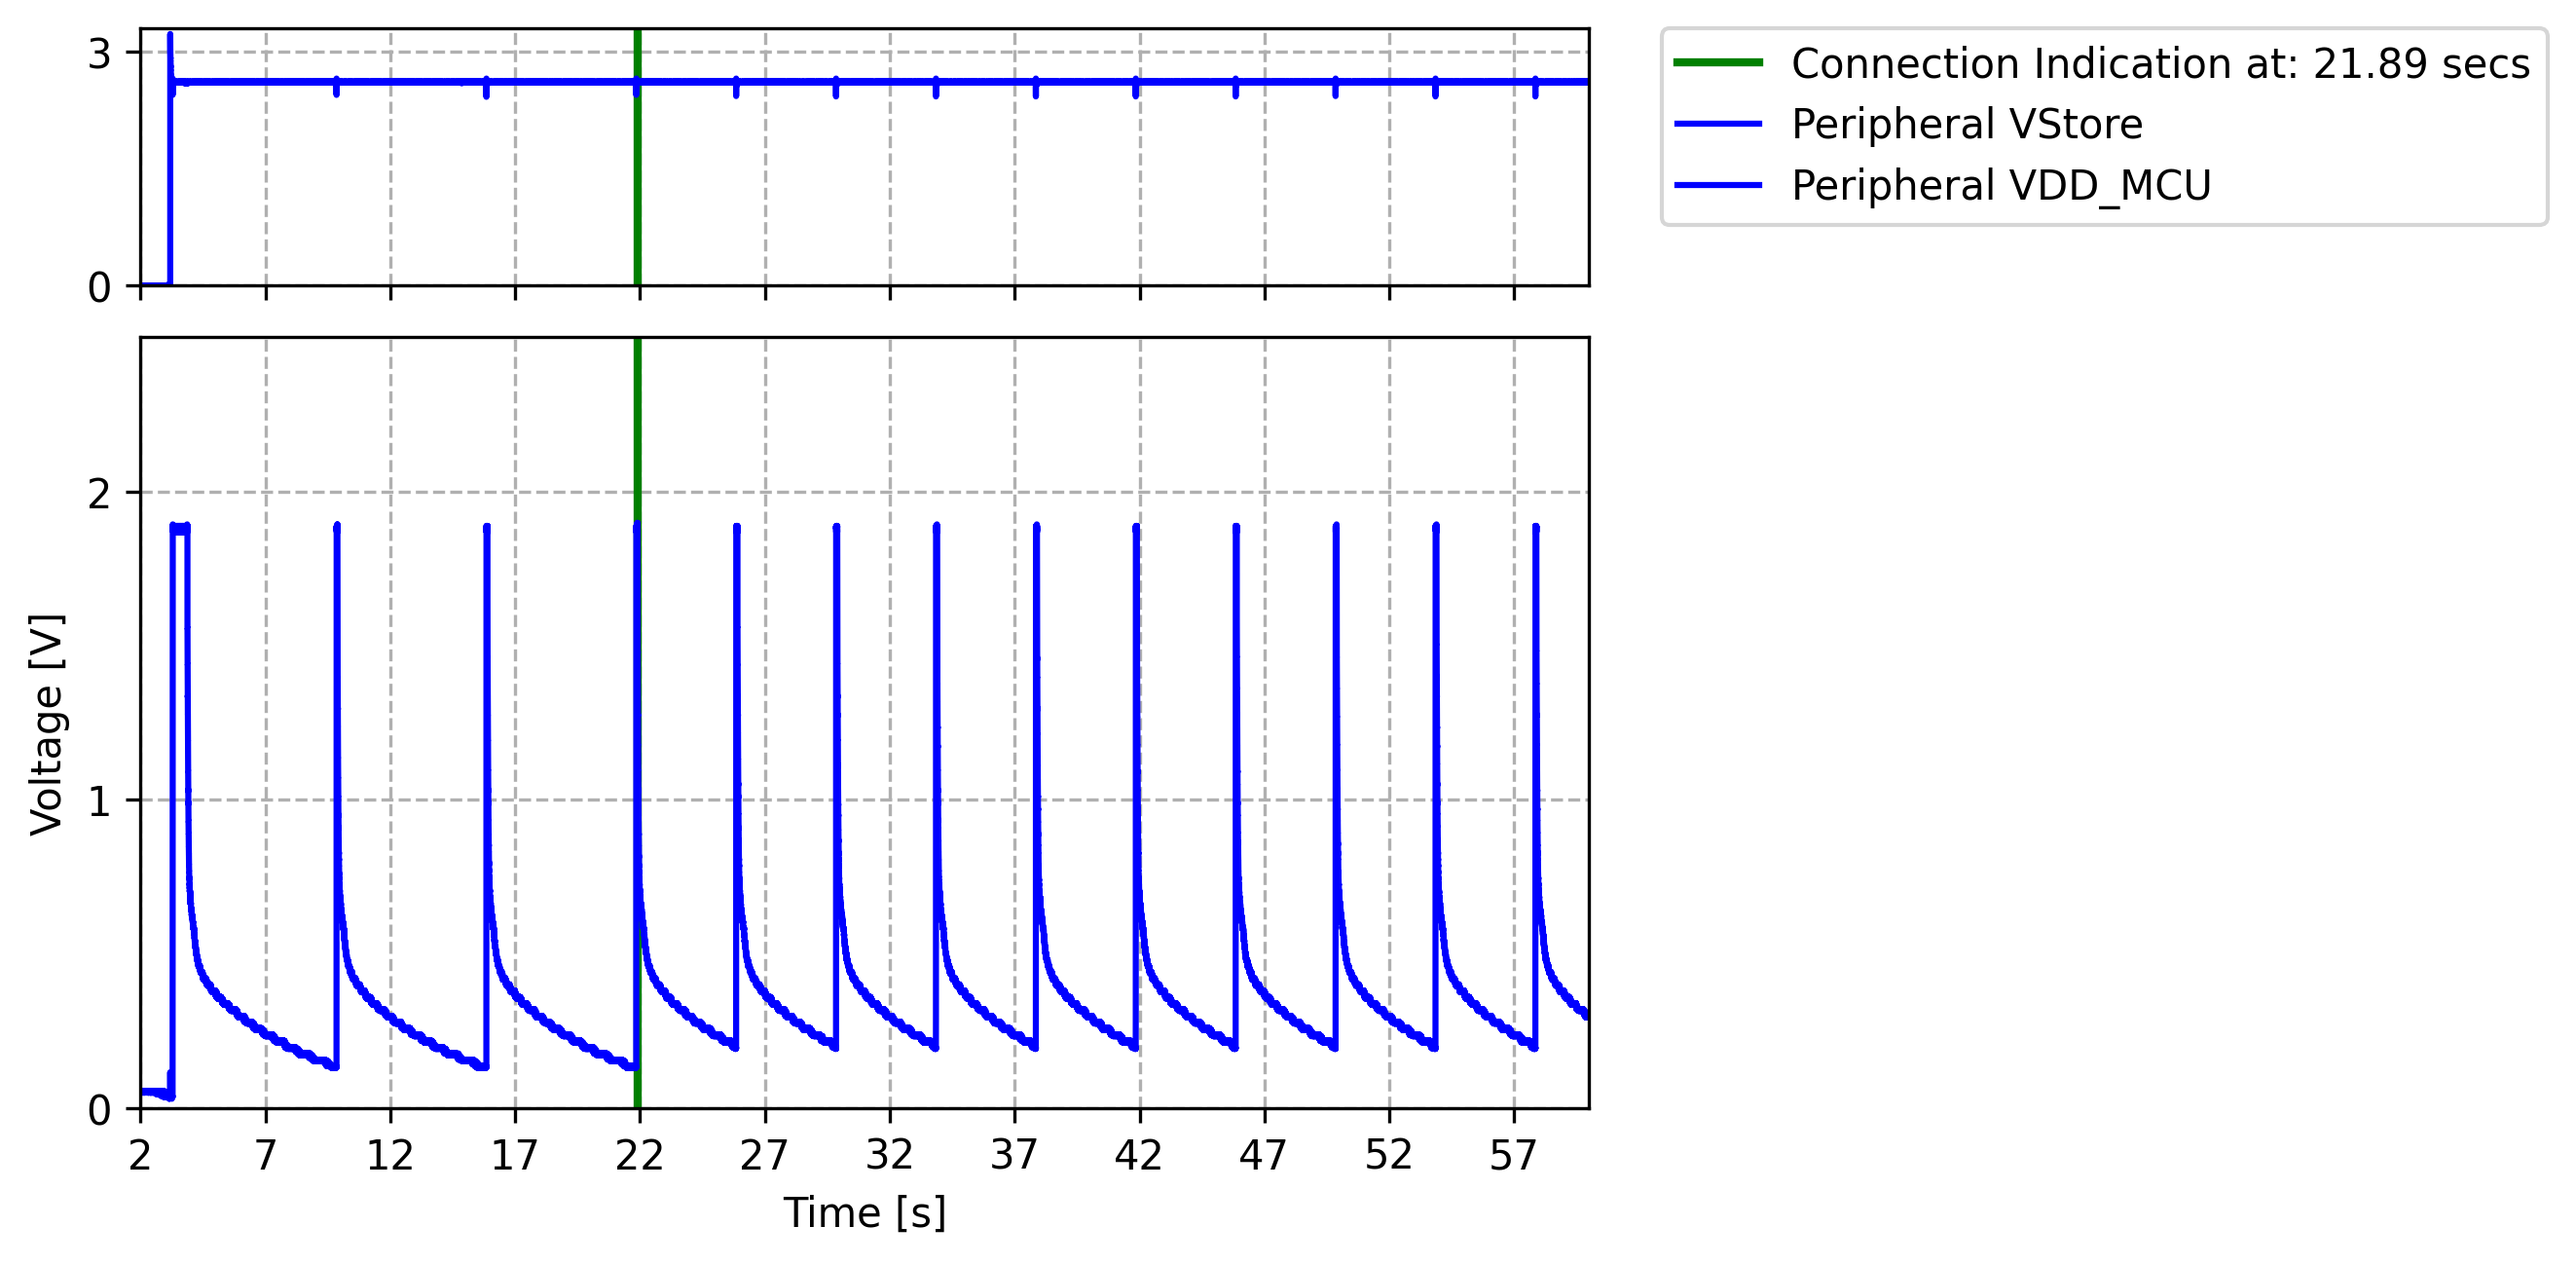
\includegraphics[width=1\linewidth]{chapters/Results/Connection_Freebie_low_peripheral.png}
        \caption{\scriptsize{FreeBie Low - Peripheral}}
        \vspace{1\baselineskip}
    \end{subfigure}\hfill
    \begin{subfigure}{0.5\linewidth}
        \centering
        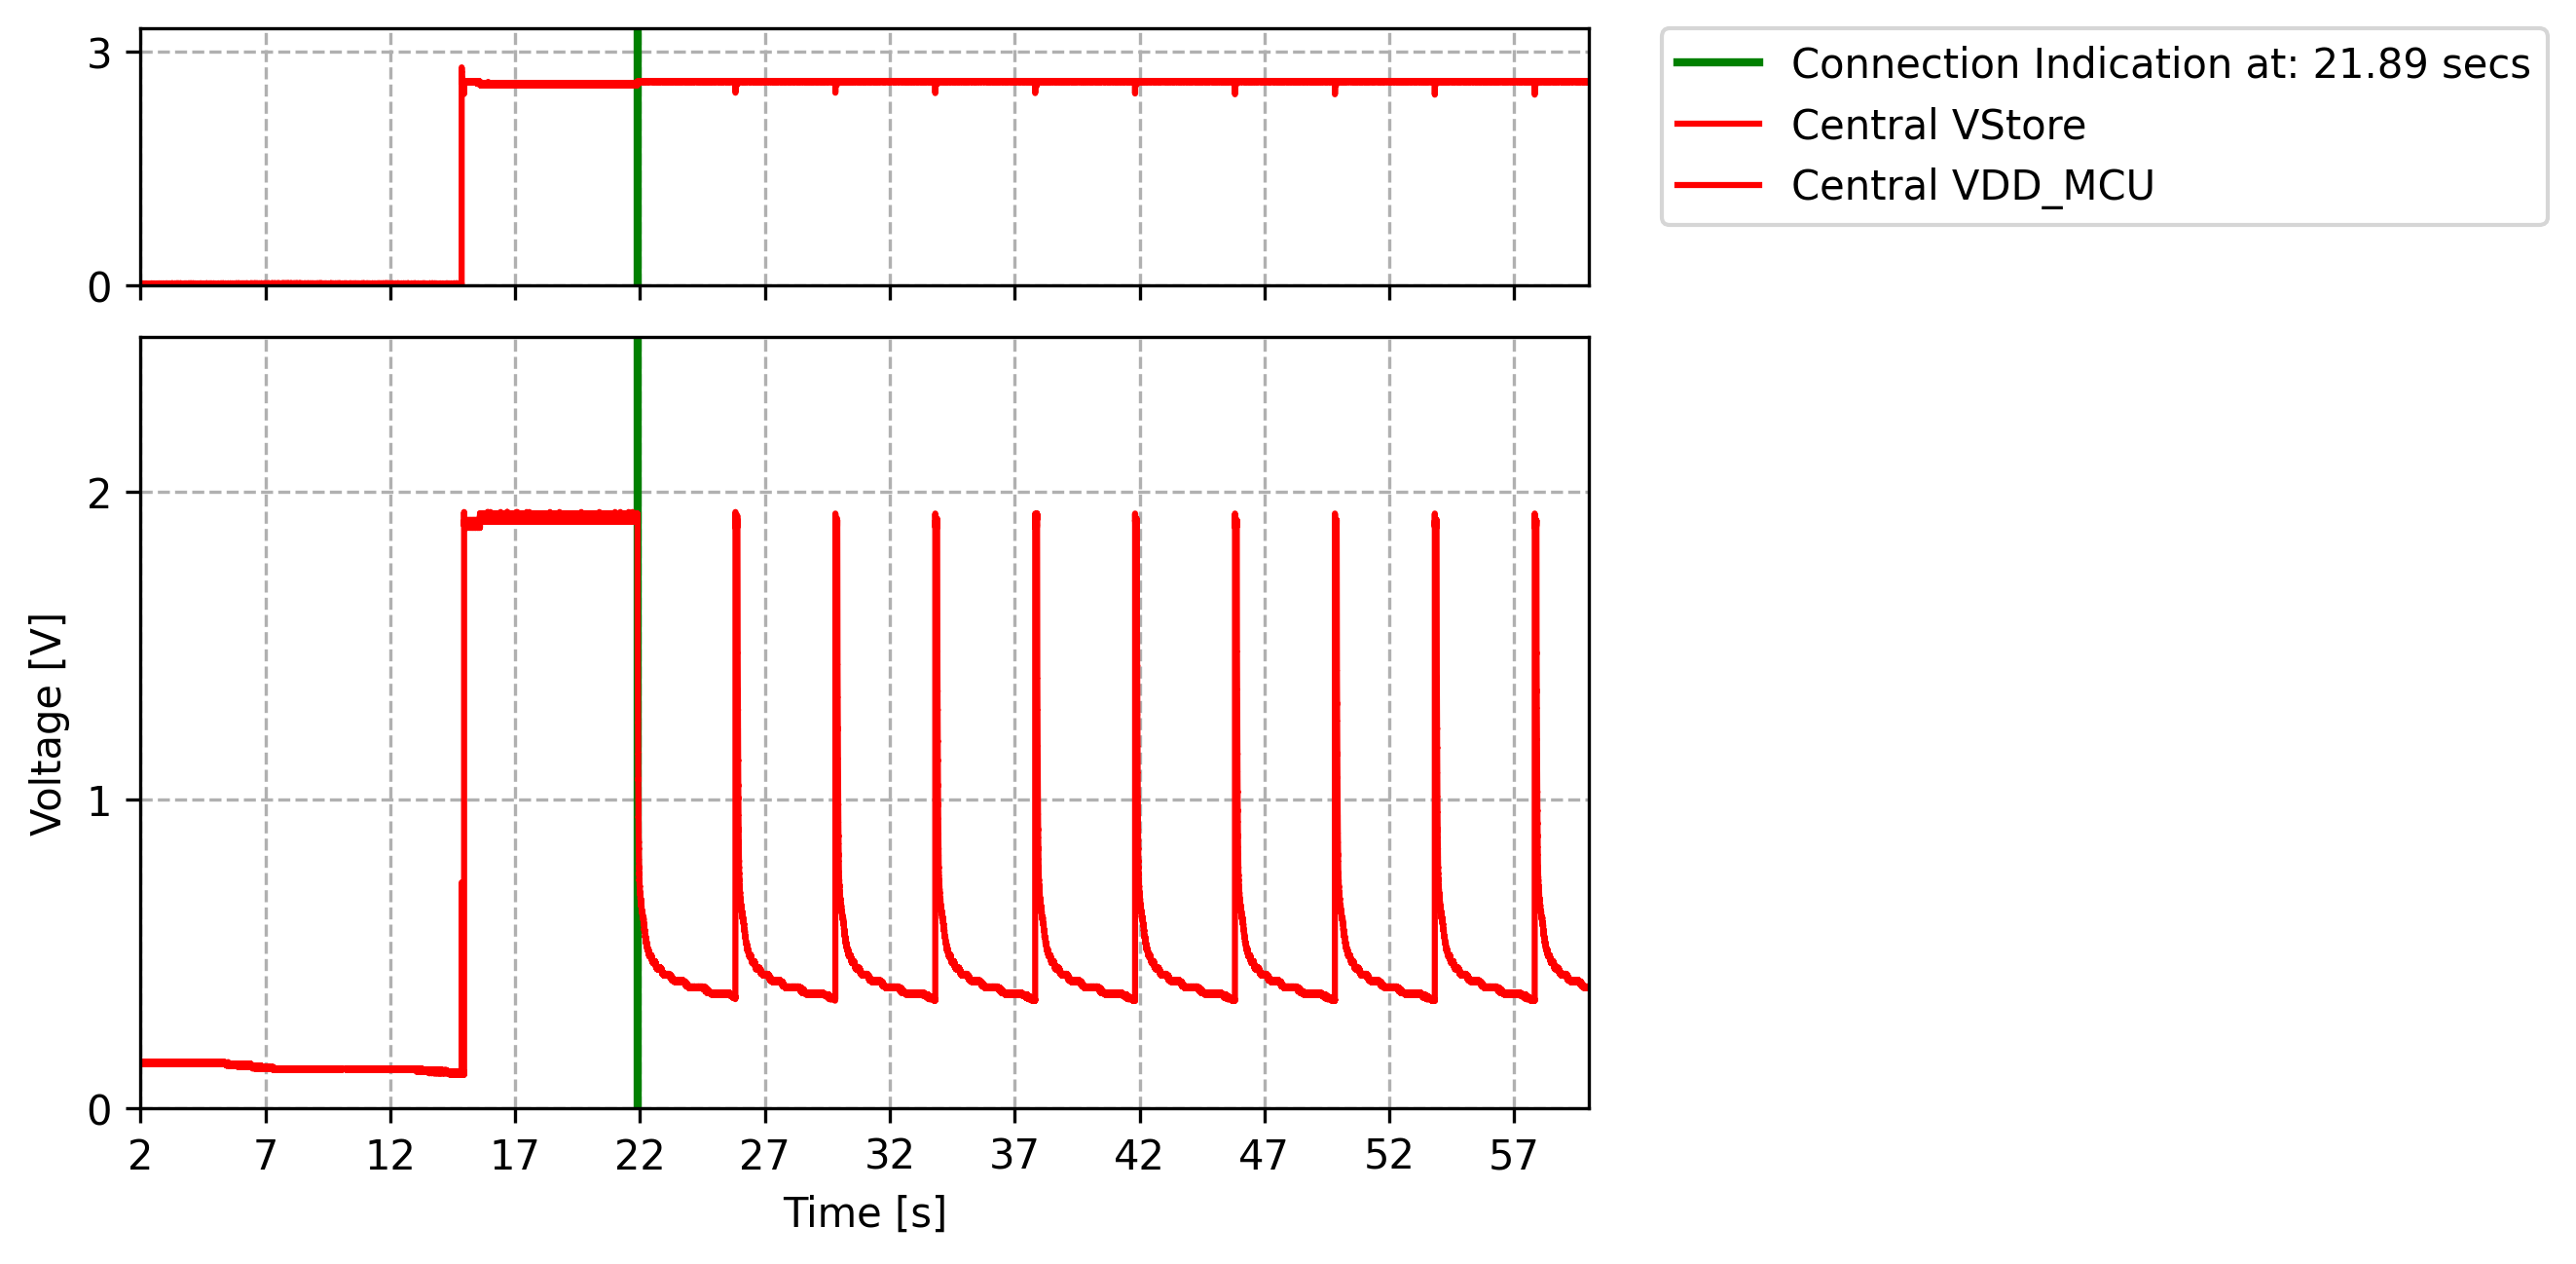
\includegraphics[width=1\linewidth]{chapters/Results/Connection_Freebie_low_central.png}
        \caption{\scriptsize{FreeBie Low - Central}}
        \vspace{1\baselineskip}
    \end{subfigure}
    \begin{subfigure}{0.5\linewidth}
        \centering
        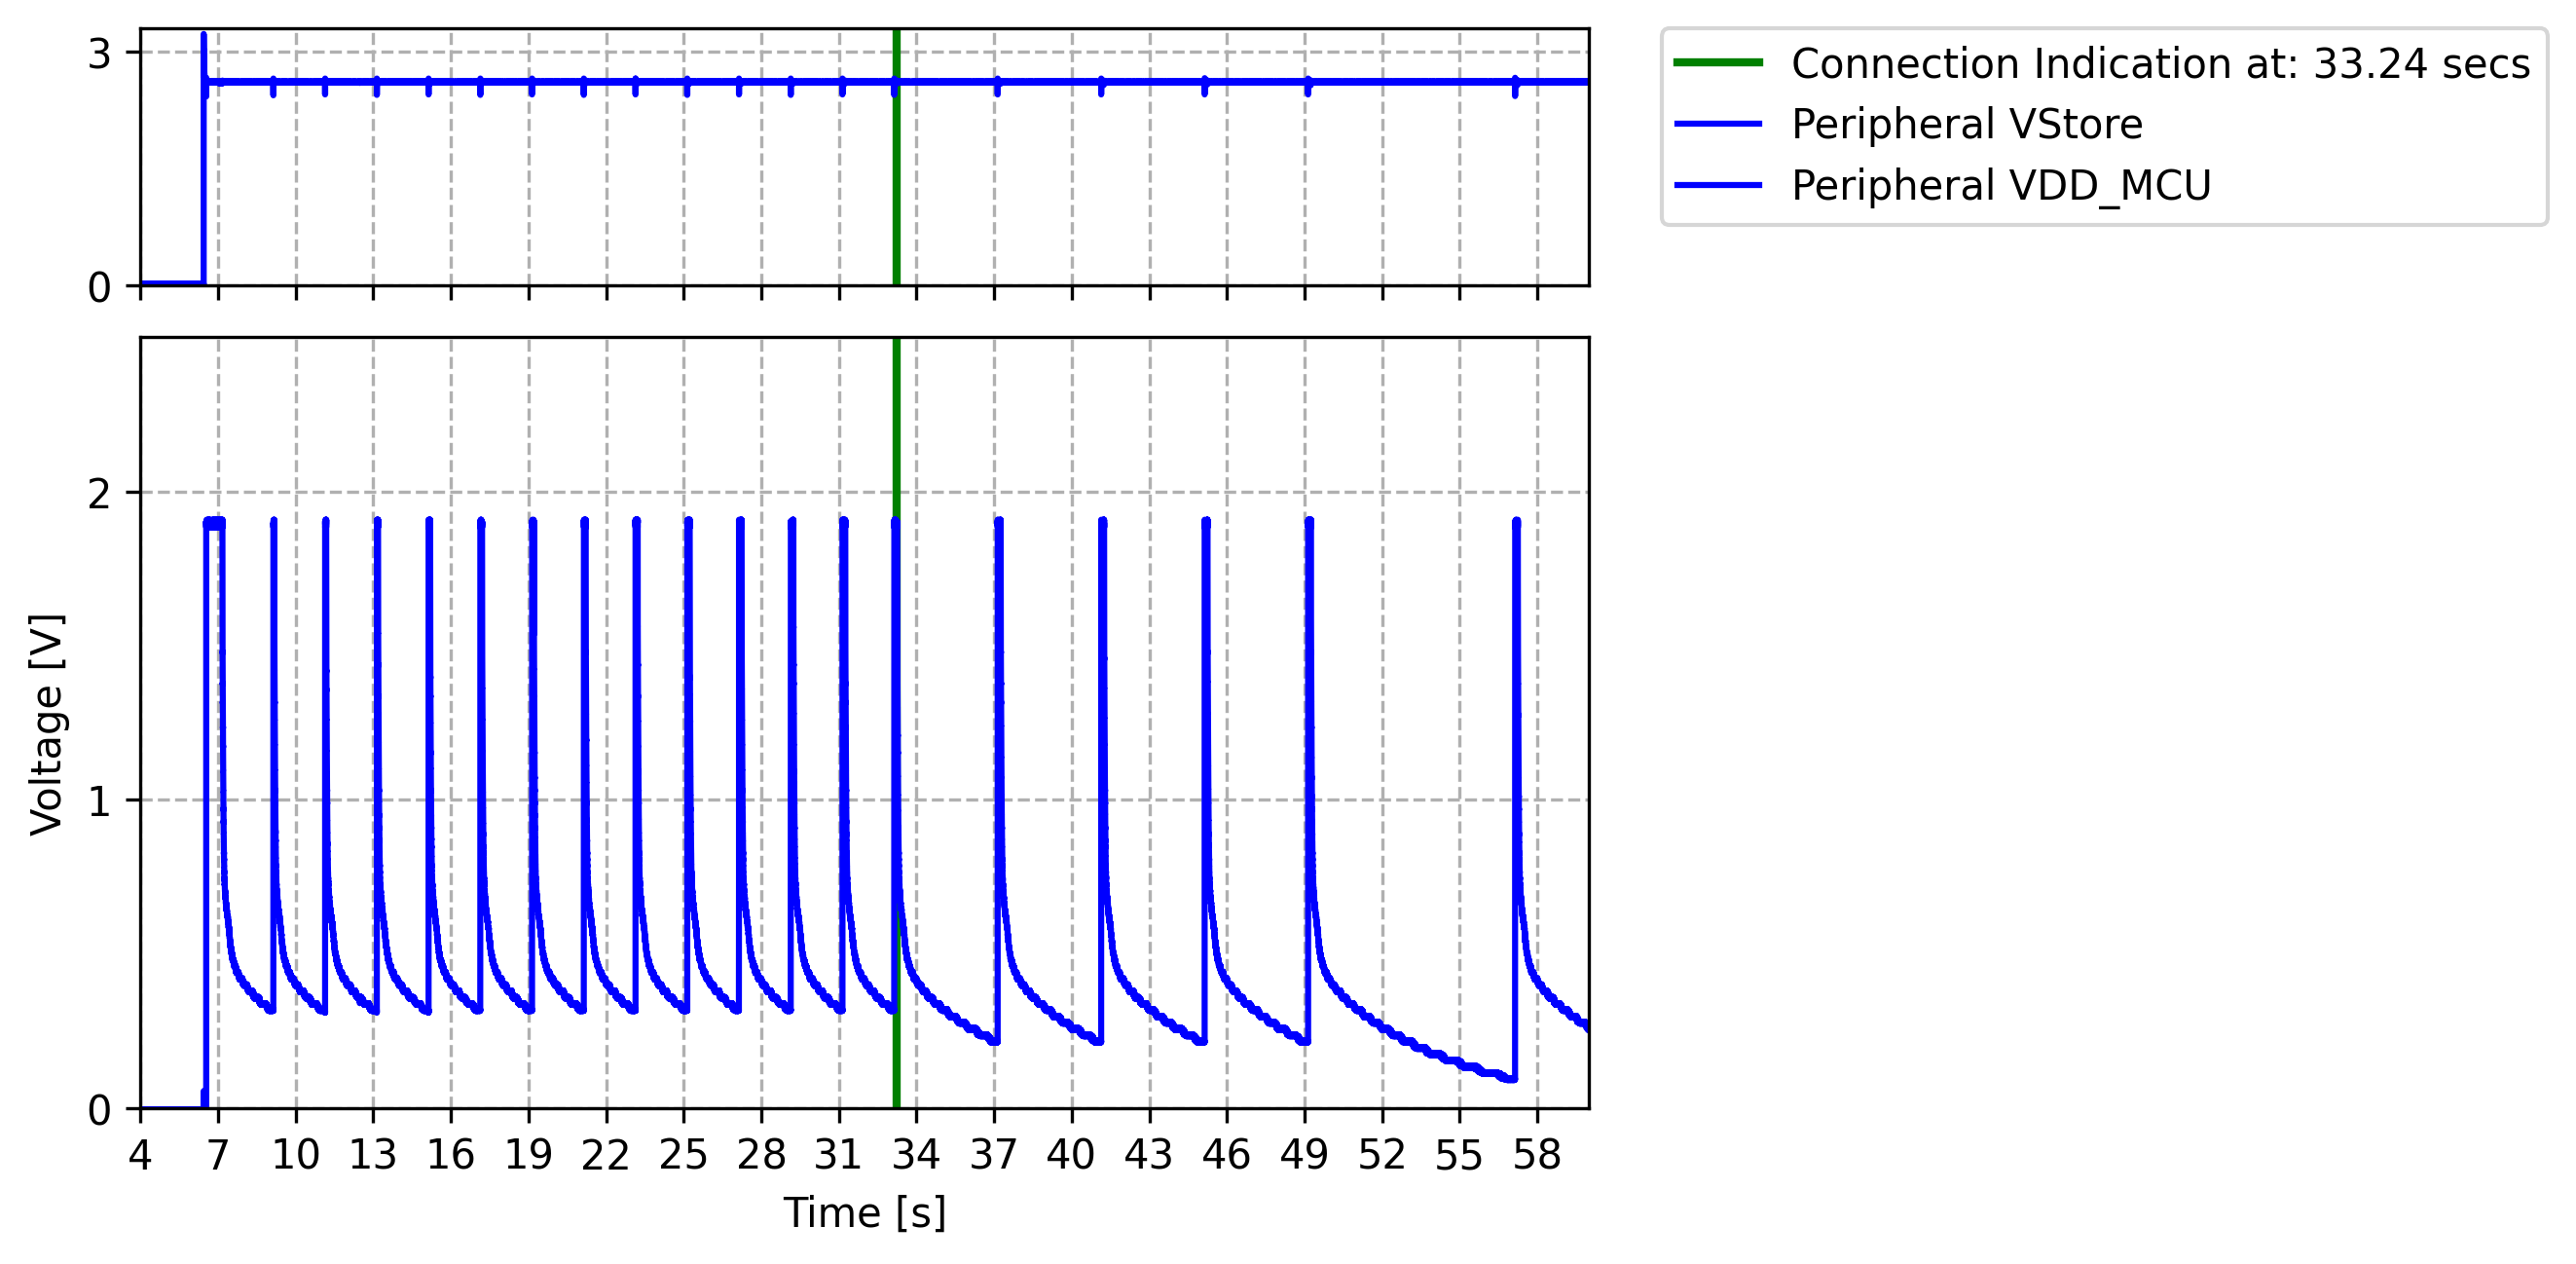
\includegraphics[width=1\linewidth]{chapters/Results/Connection_Freebie_medium_peripheral.png}
        \caption{\scriptsize{FreeBie Medium - Peripheral}}
        \vspace{1\baselineskip}
    \end{subfigure}\hfill
    \begin{subfigure}{0.5\linewidth}
        \centering
        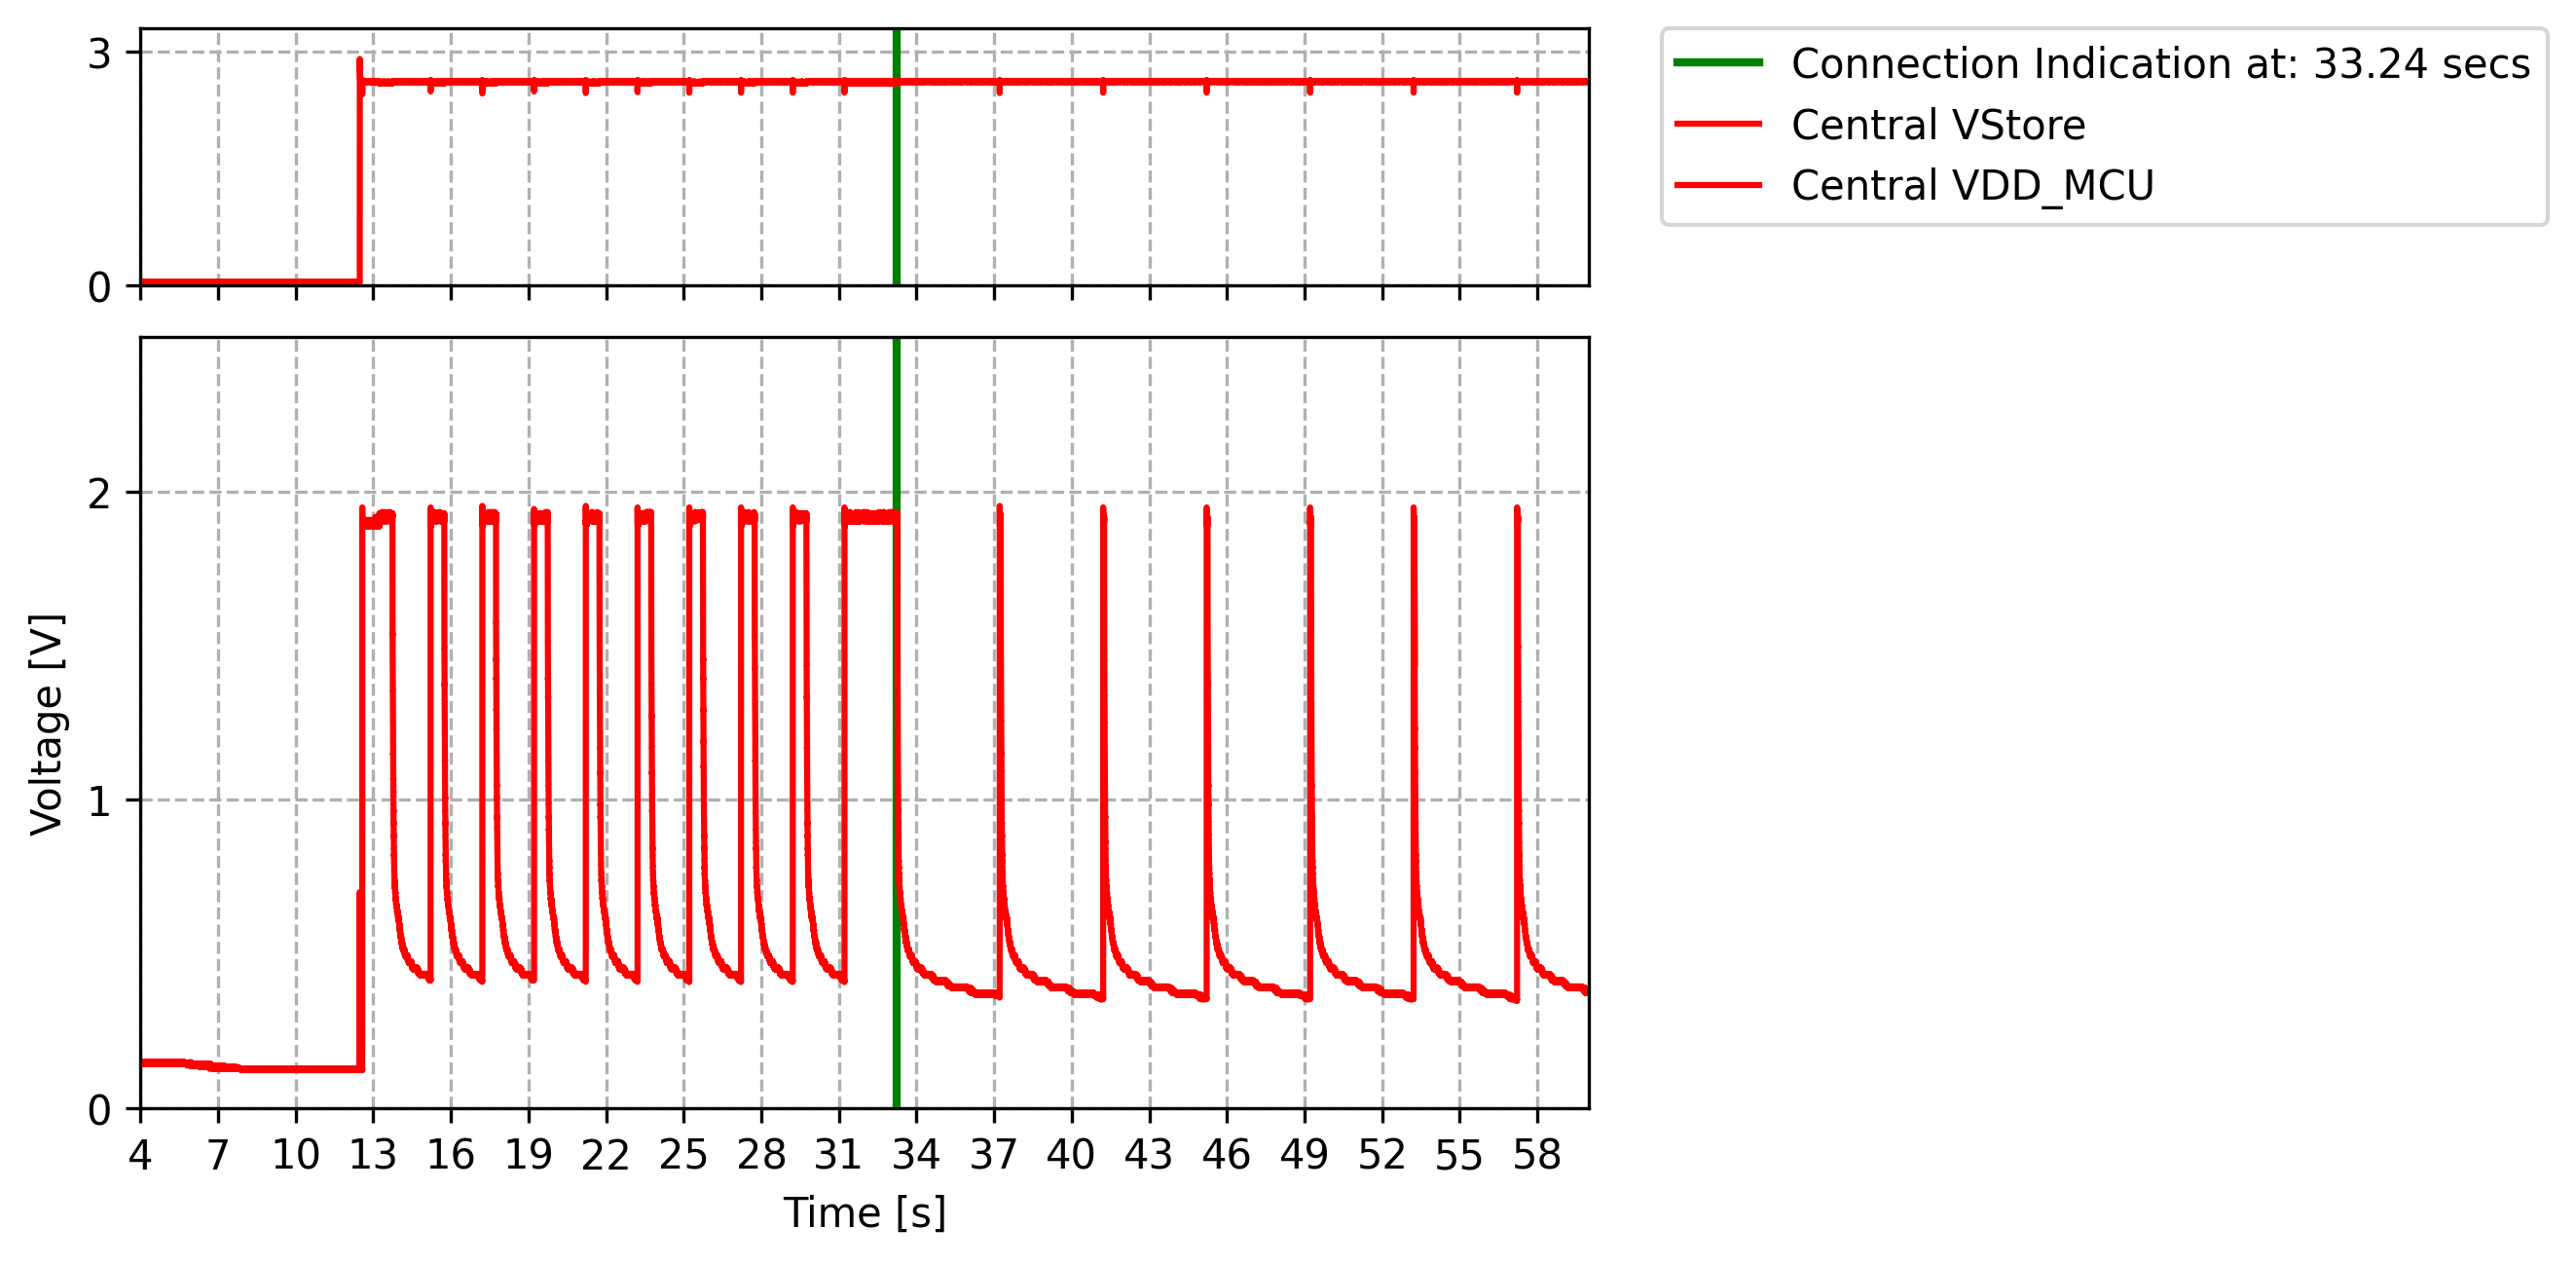
\includegraphics[width=1\linewidth]{chapters/Results/Connection_Freebie_medium_central.png}
        \caption{\scriptsize{FreeBie Medium - Central}}
        \vspace{1\baselineskip}
    \end{subfigure}
    \begin{subfigure}{0.5\linewidth}
        \centering
        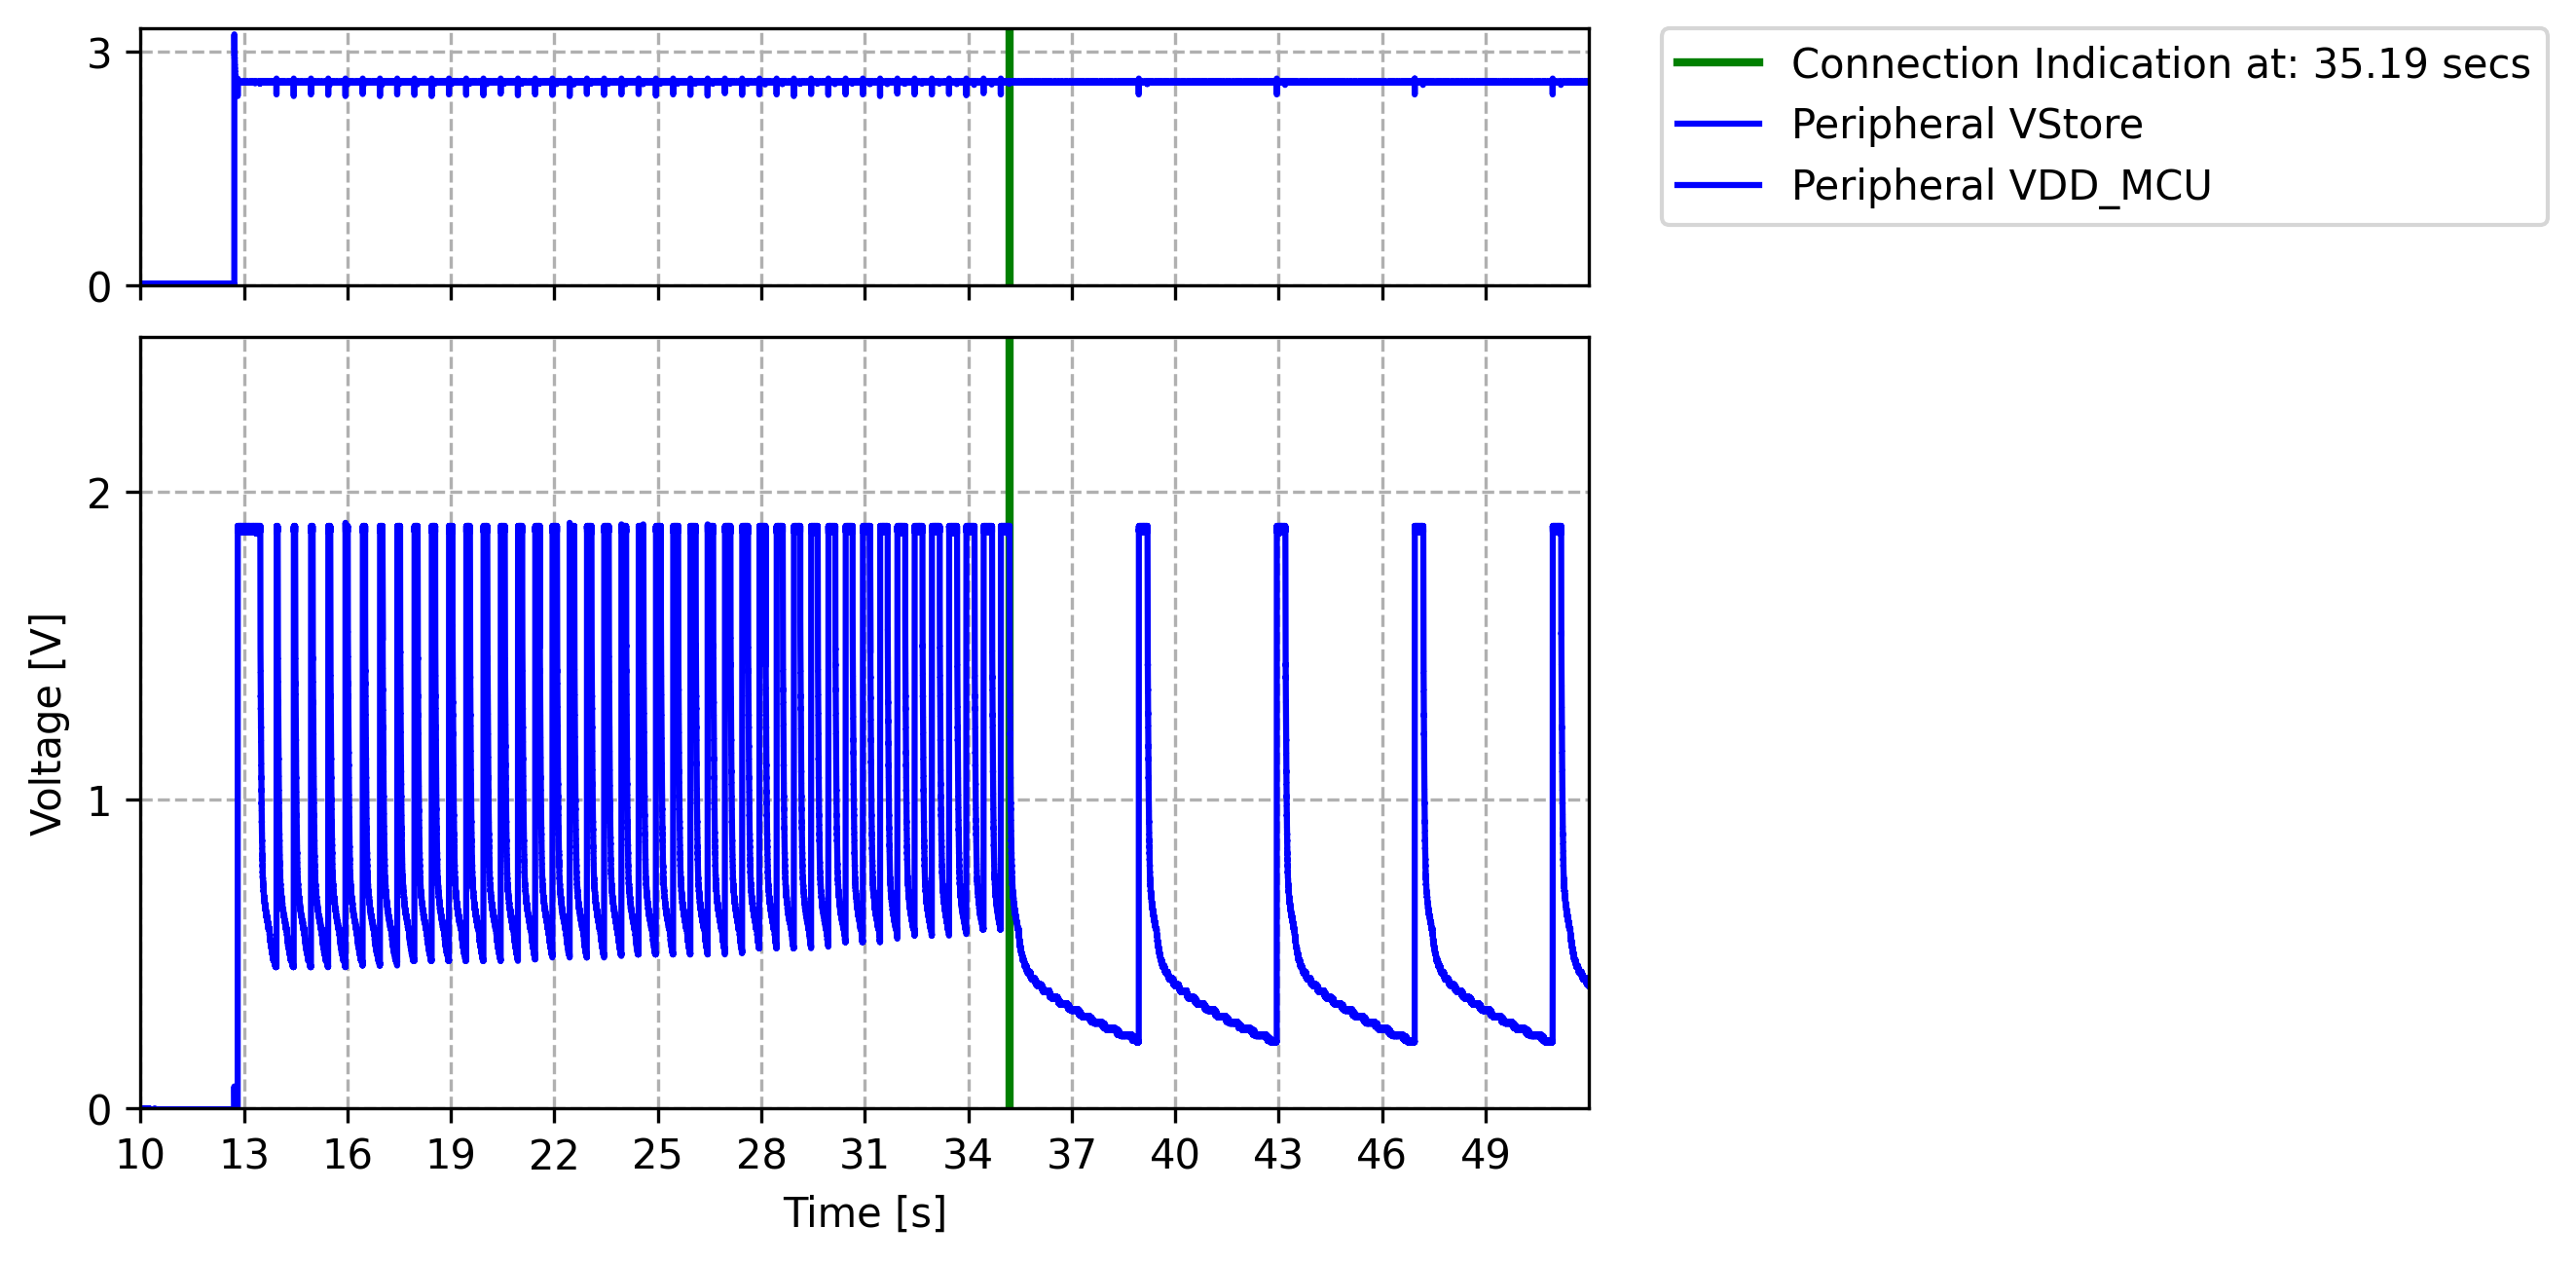
\includegraphics[width=1\linewidth]{chapters/Results/Connection_Freebie_high_peripheral.png}
        \caption{\scriptsize{FreeBie High - Peripheral}}
    \end{subfigure} \hfill
    \begin{subfigure}{0.5\linewidth}
        \centering
        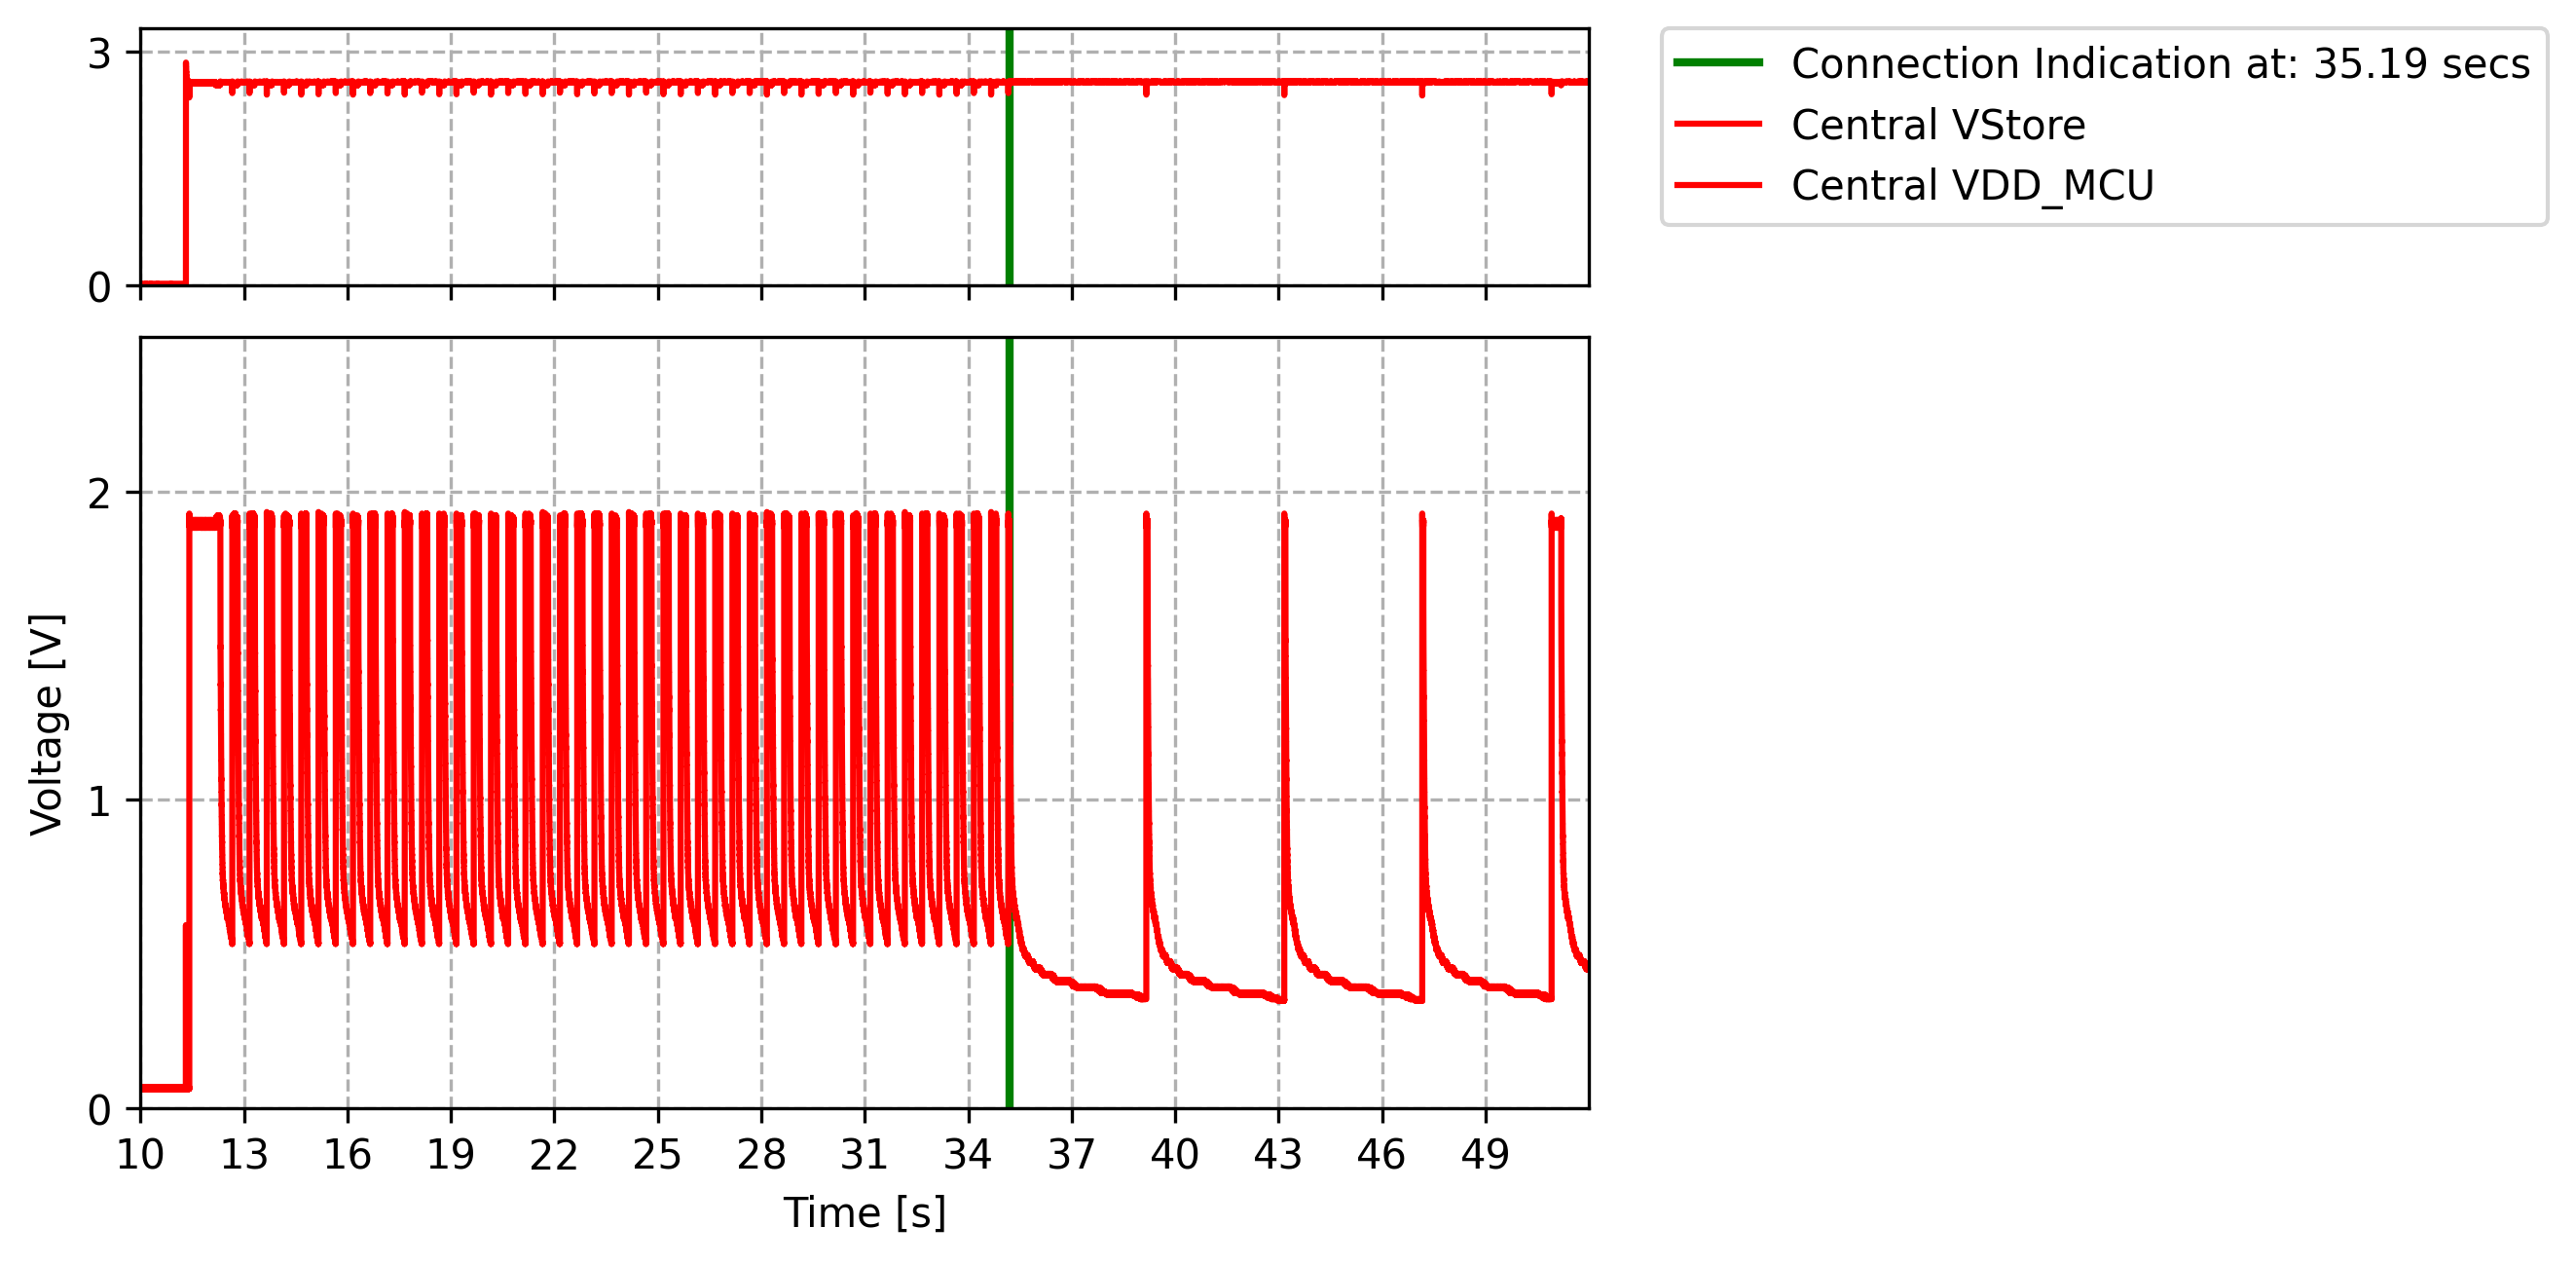
\includegraphics[width=1\linewidth]{chapters/Results/Connection_Freebie_high_central.png}
        \caption{\scriptsize{FreeBie High - Central device}}
    \end{subfigure}         
    \caption{Real-time voltage measurement of FreeBie system. Each of the two plots in both devices for each configuration shows different measurements. From top to bottom in each device, 1) Plot of \(\text{V}_\text{Store}\) : Supply Voltage and 2) Plot of \(\text{V}_\text{DD\_MCU}\) : MCU voltage. The green vertical line through all the plots indicates the successful BLE connection setup event.}
    \label{fig:voltage_freebie}
\end{figure}
\begin{figure}[t]
    \begin{subfigure}{0.45\linewidth}
        \centering
        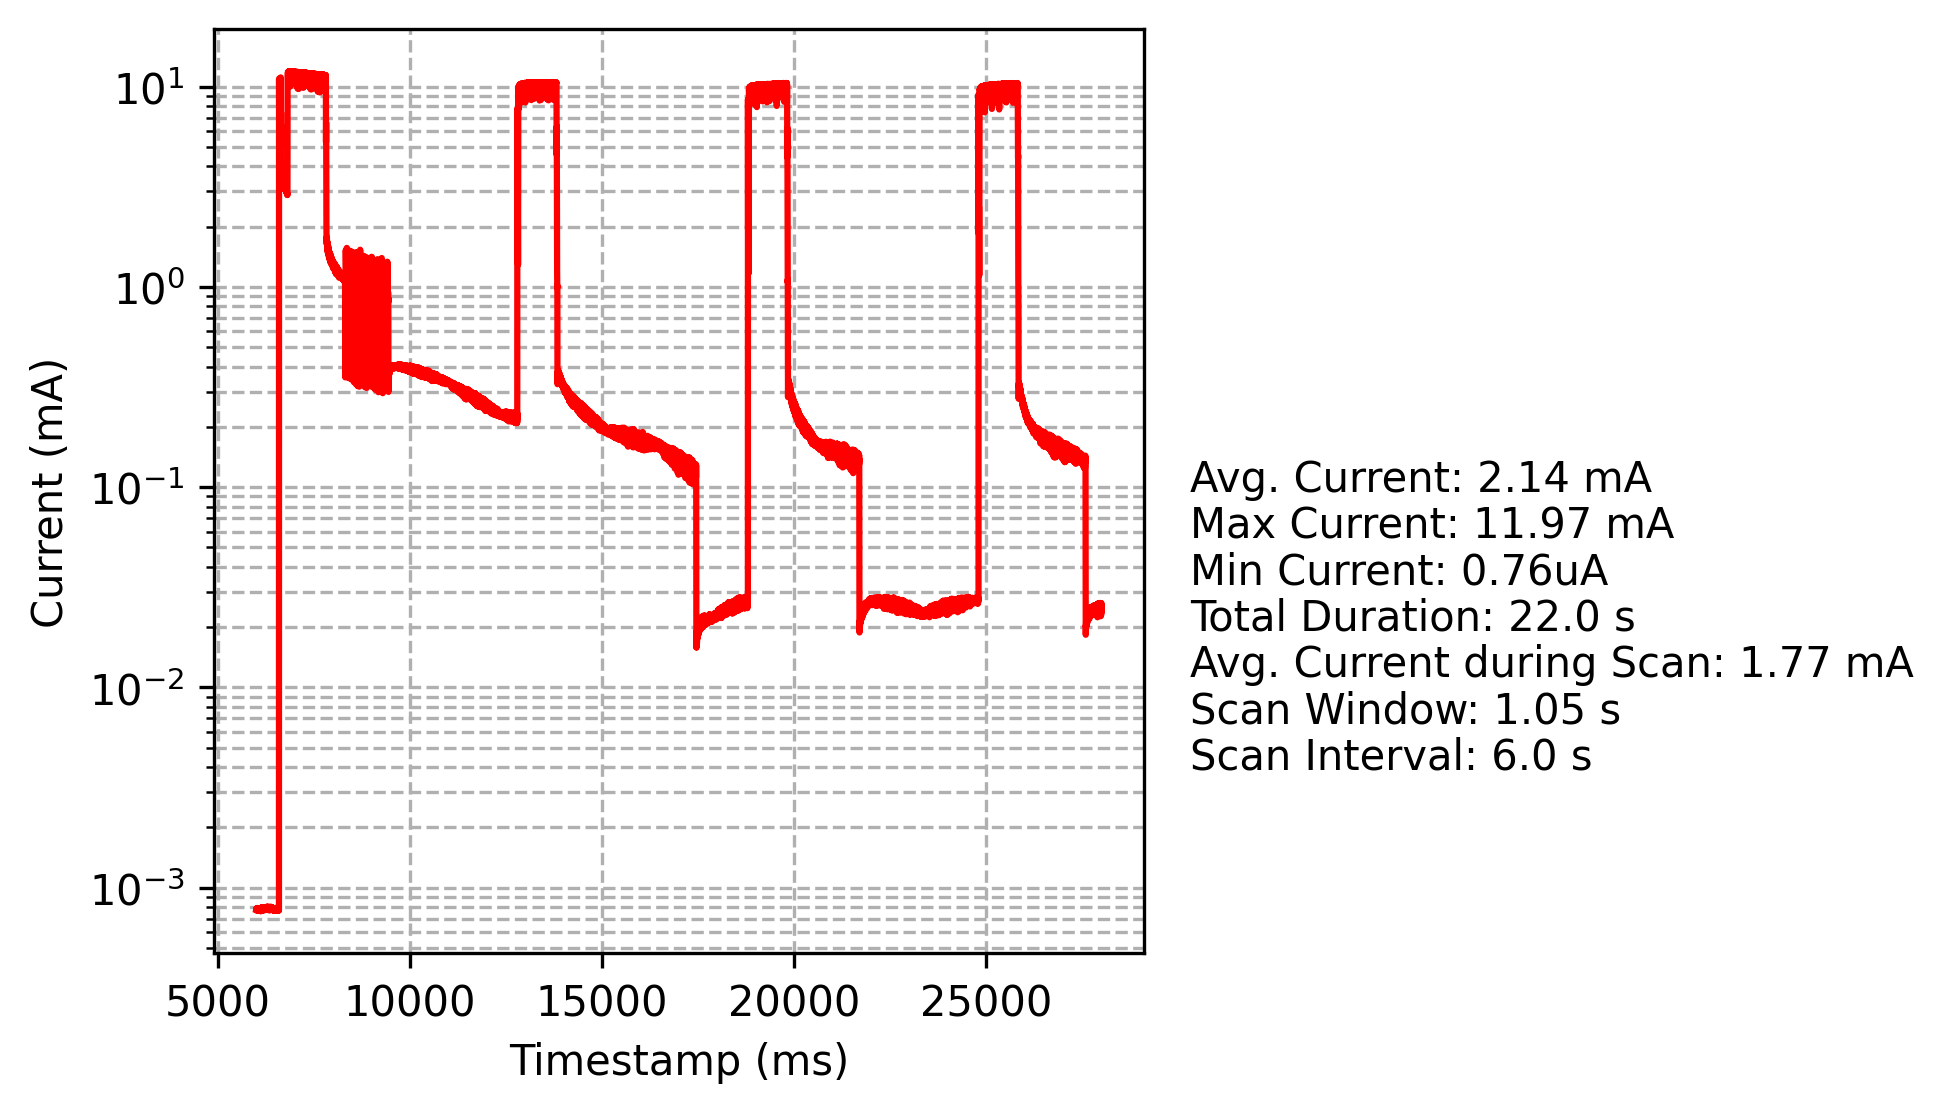
\includegraphics[width=\linewidth]{chapters/Results/Current vs Timestamp - FreeBie Central Low.png}
        \caption{FreeBie Low - Central}
        \label{fig:freebie_low_central}
    \end{subfigure}\hfill
    \begin{subfigure}{0.45\linewidth}
        \centering
        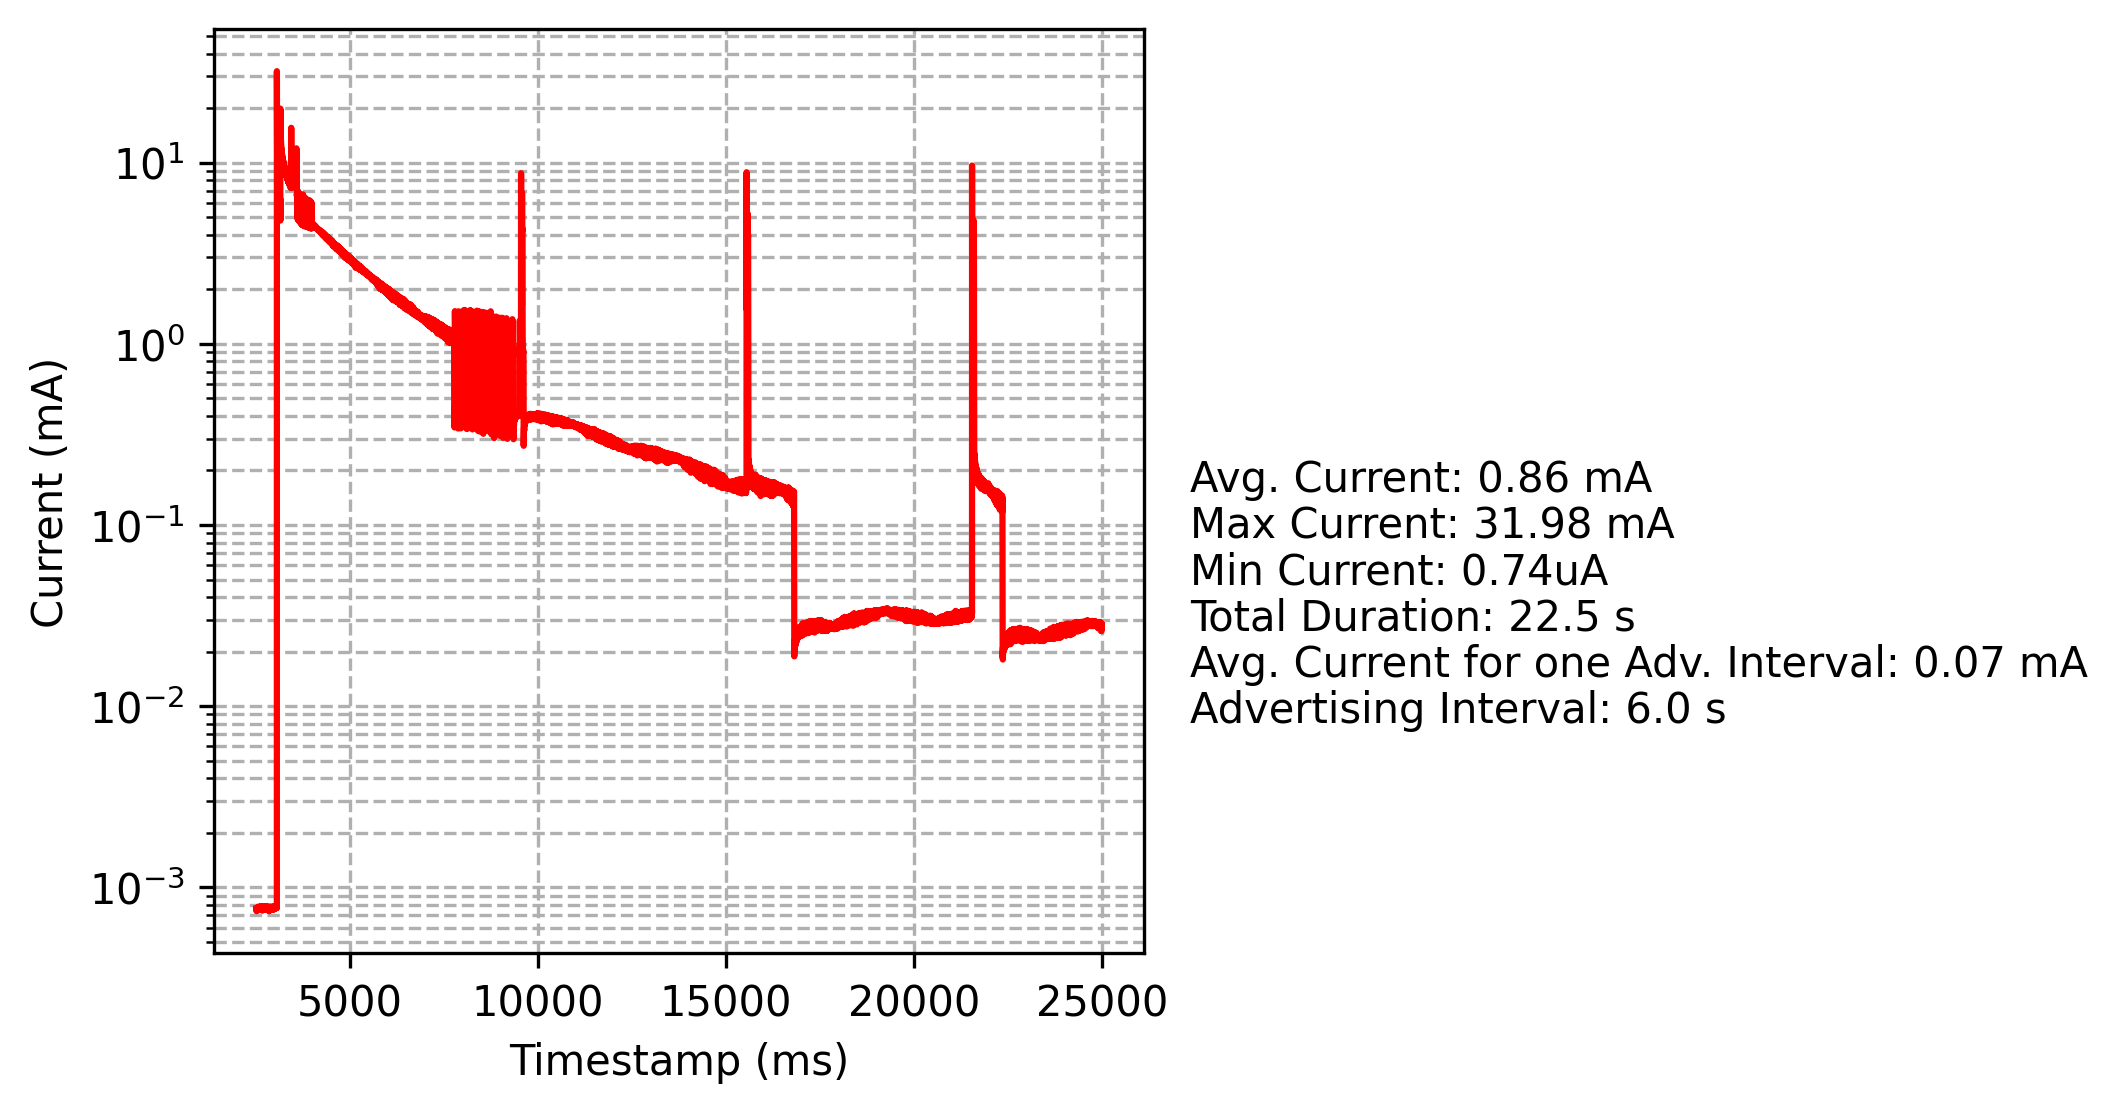
\includegraphics[width=\linewidth]{chapters/Results/Current vs Timestamp - FreeBie Peripheral Low.png}
        \caption{FreeBie Low - Peripheral}
        \label{fig:freebie_low_peripheral}
    \end{subfigure}
    \begin{subfigure}{0.45\linewidth}
        \centering
        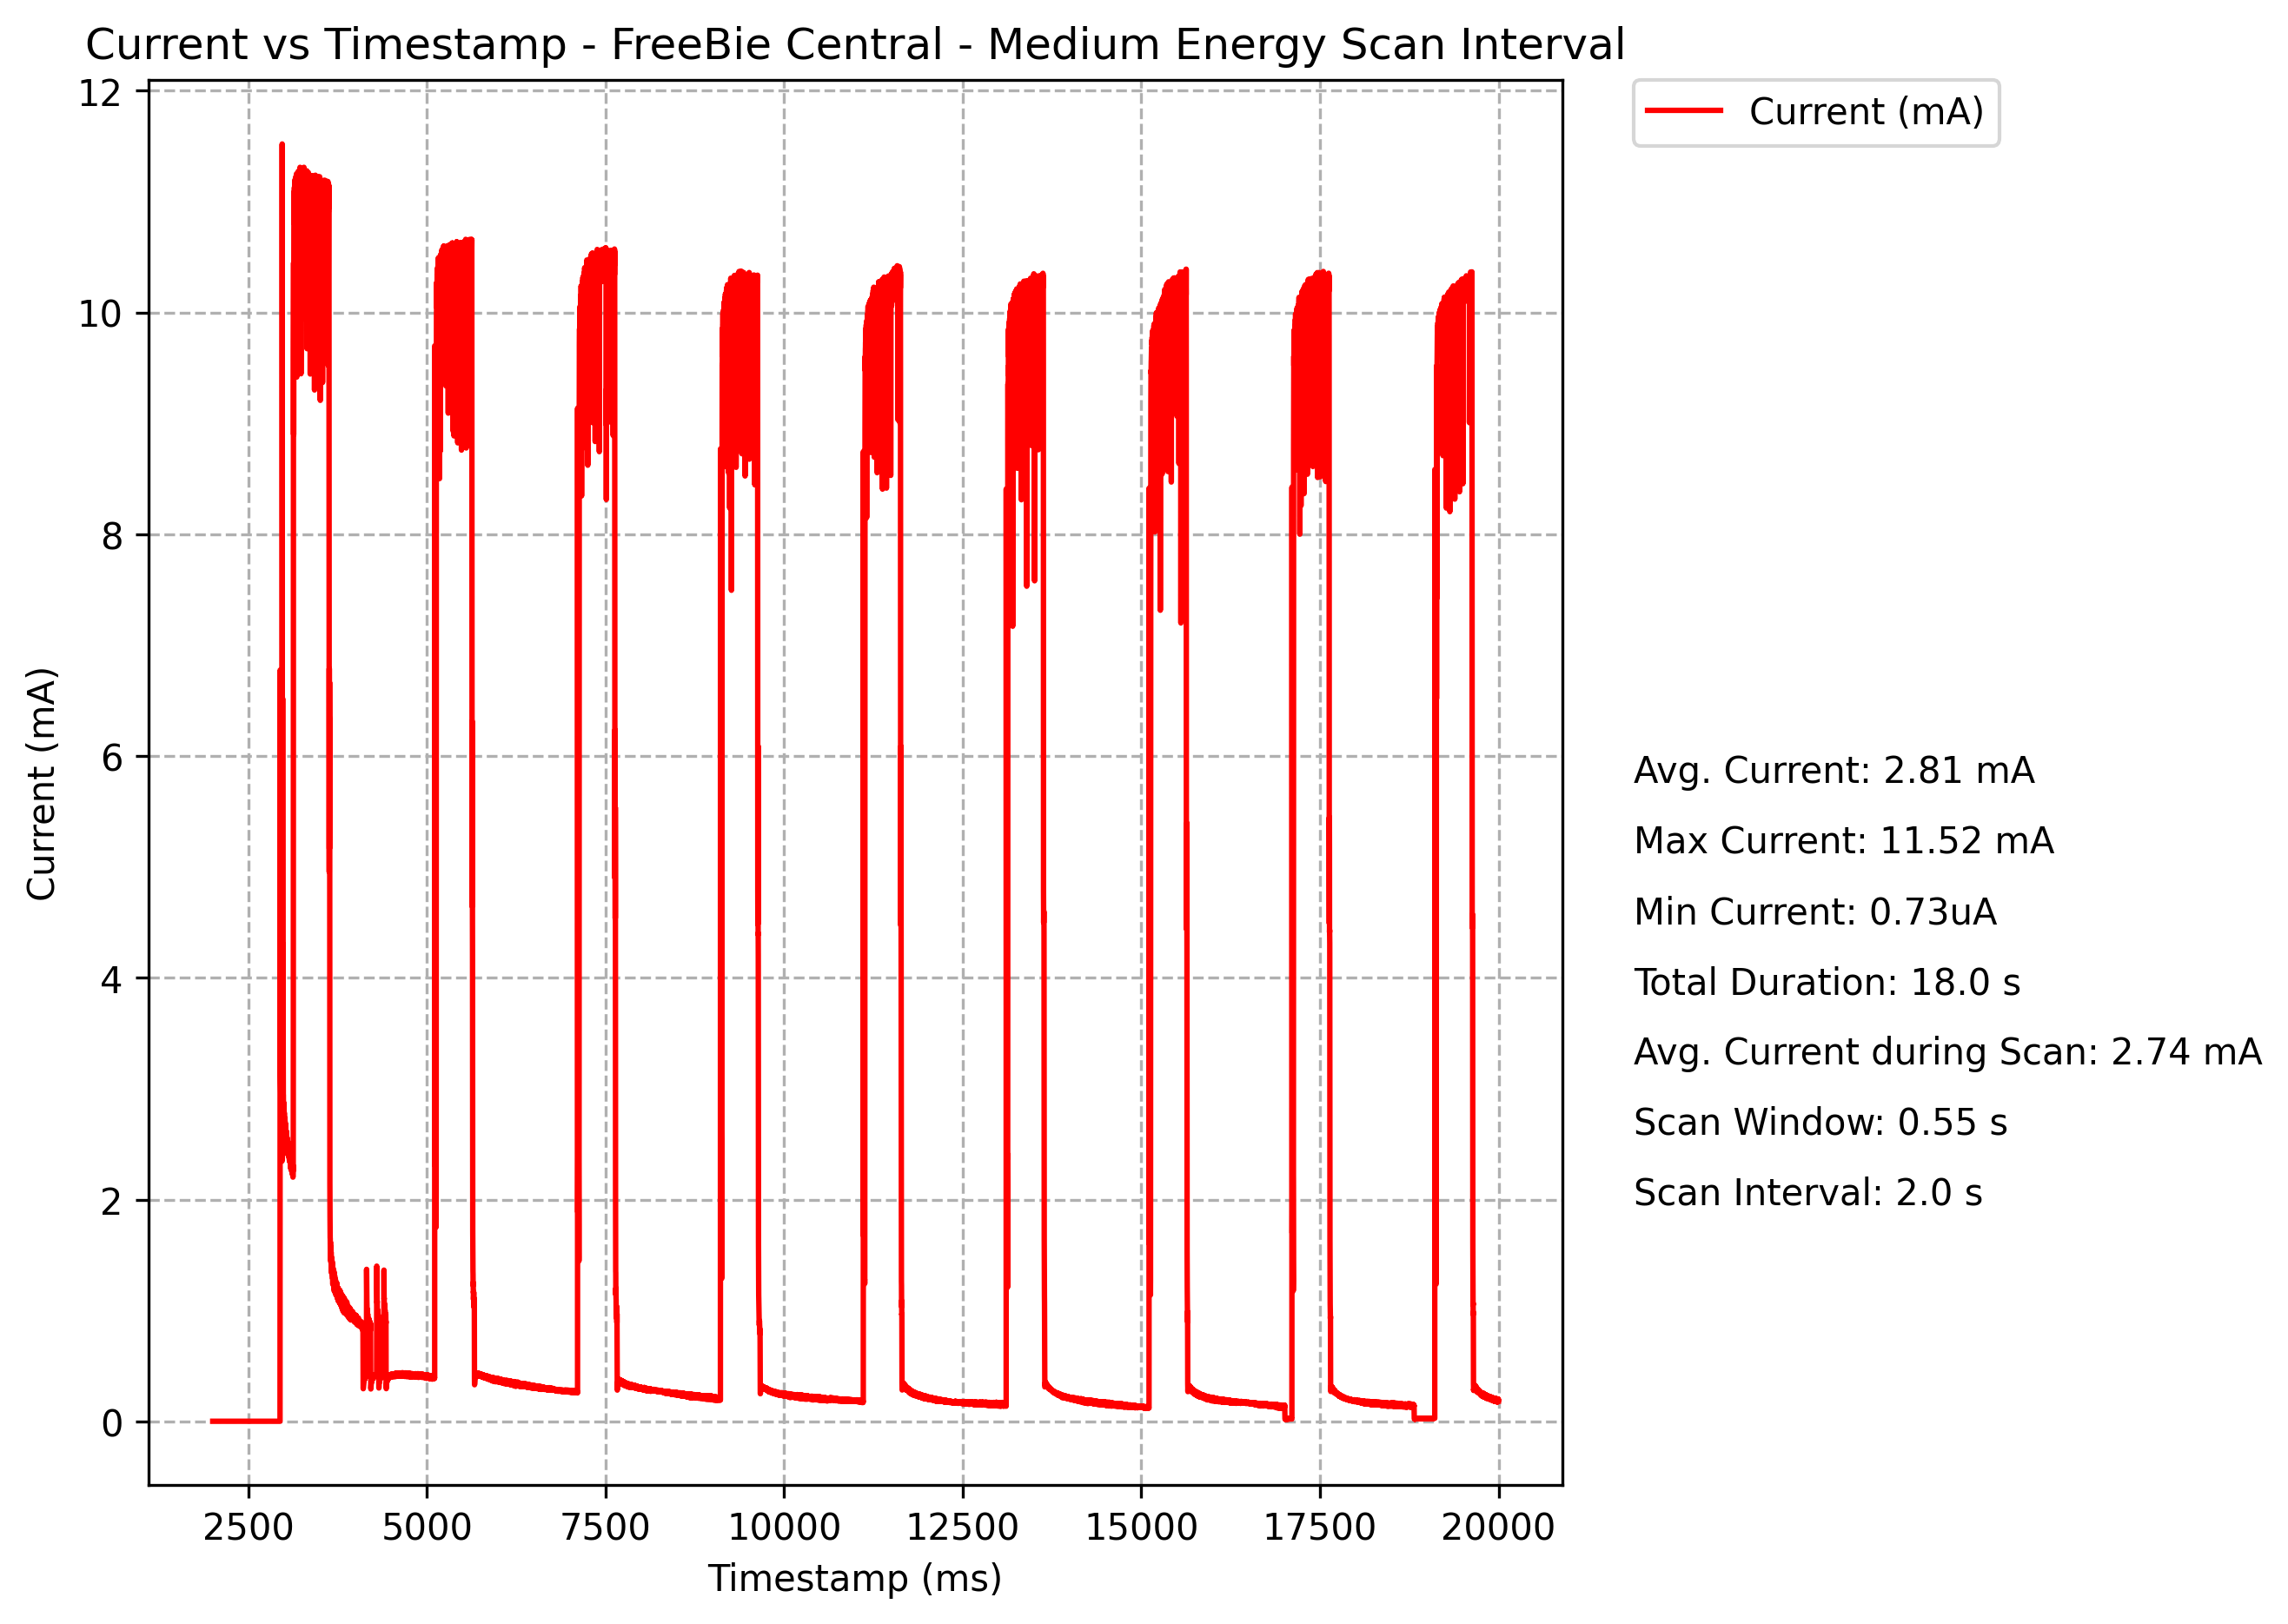
\includegraphics[width=\linewidth]{chapters/Results/Current vs Timestamp - FreeBie Central Medium.png}
        \caption{FreeBie Medium- Central}
        \label{fig:freebie_medium_central}
    \end{subfigure}\hfill
    \begin{subfigure}{0.45\linewidth}
        \centering
        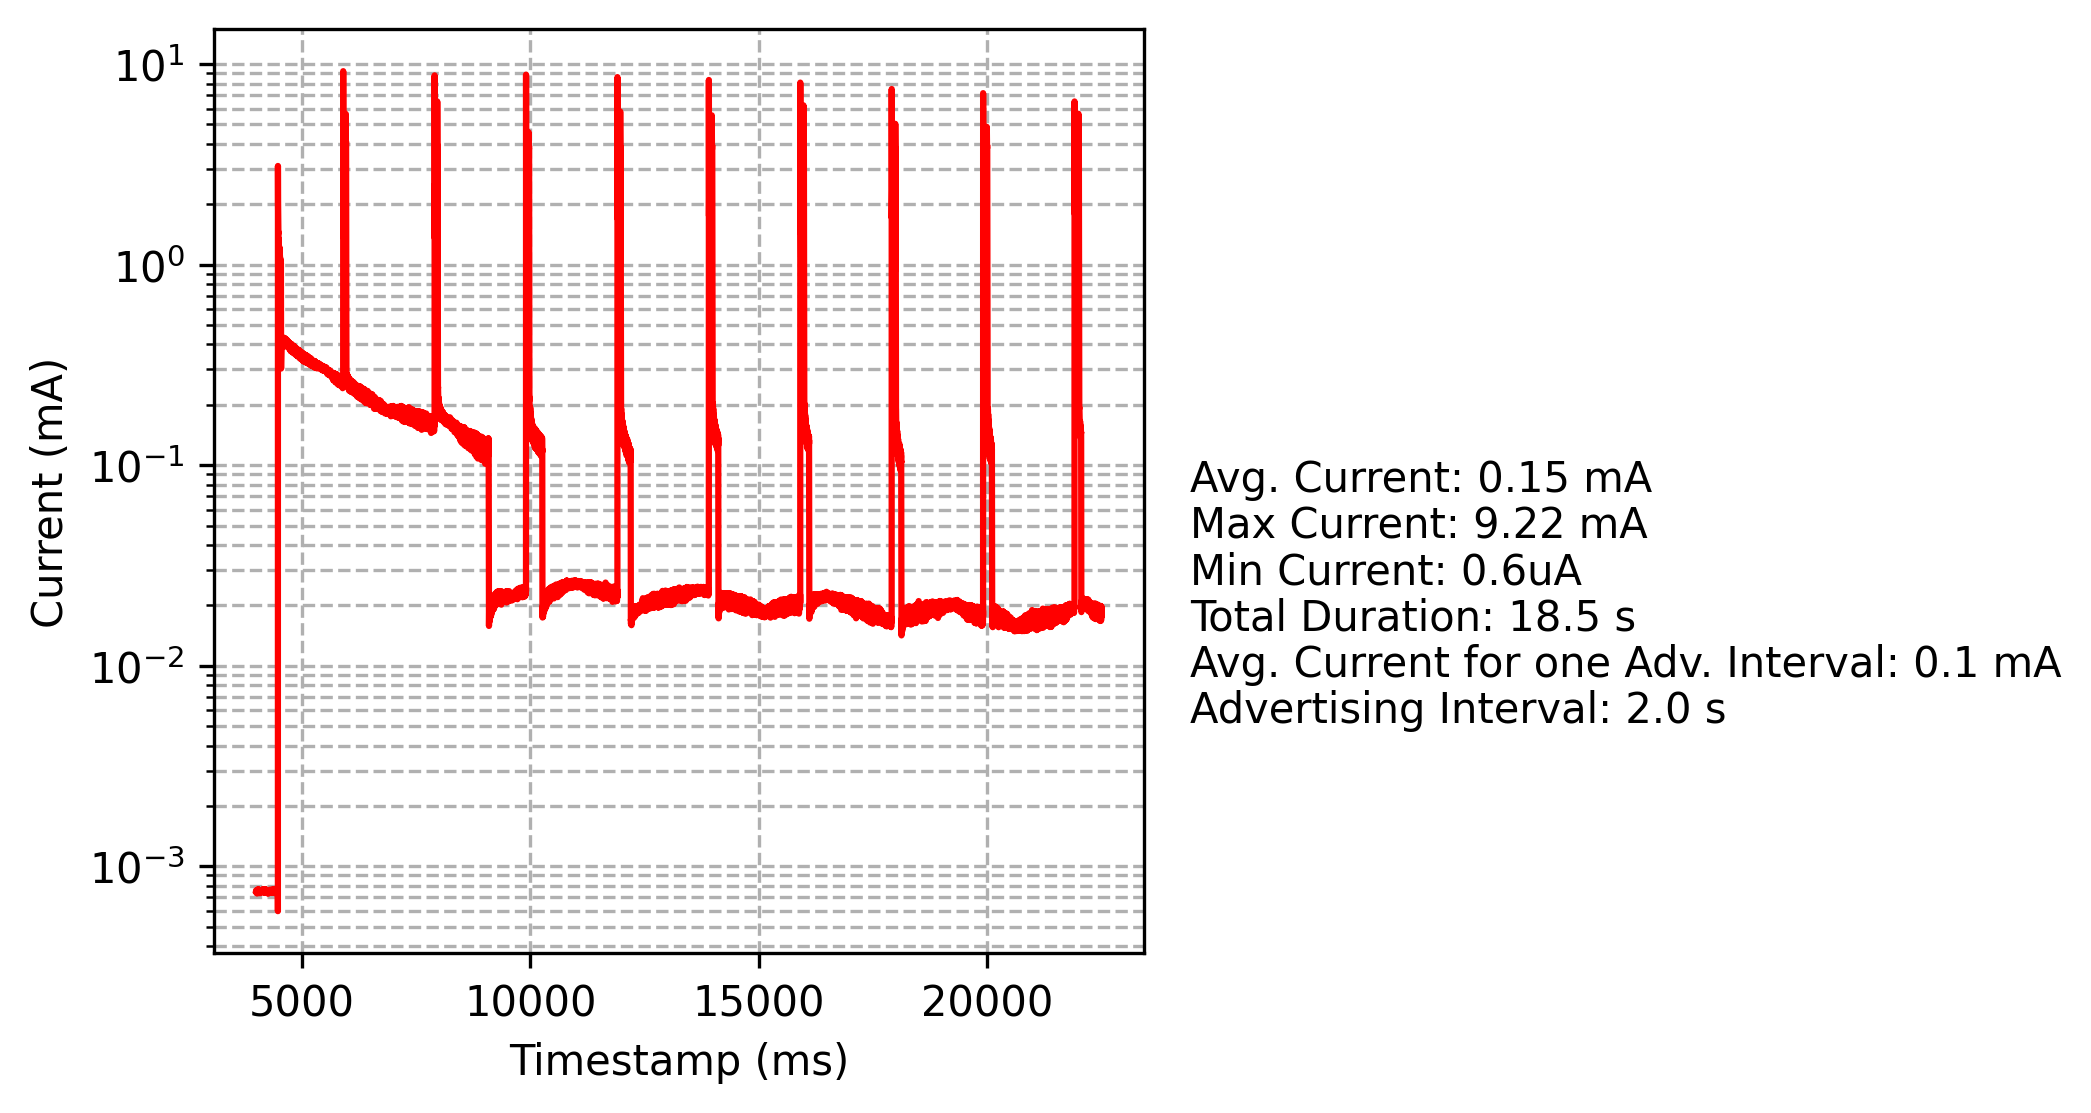
\includegraphics[width=\linewidth]{chapters/Results/Current vs Timestamp - FreeBie Peripheral Medium.png}
        \caption{FreeBie Medium - Peripheral}
        \label{fig:freebie_medium_peripheral}
    \end{subfigure}
    \begin{subfigure}{0.45\linewidth}
        \centering
        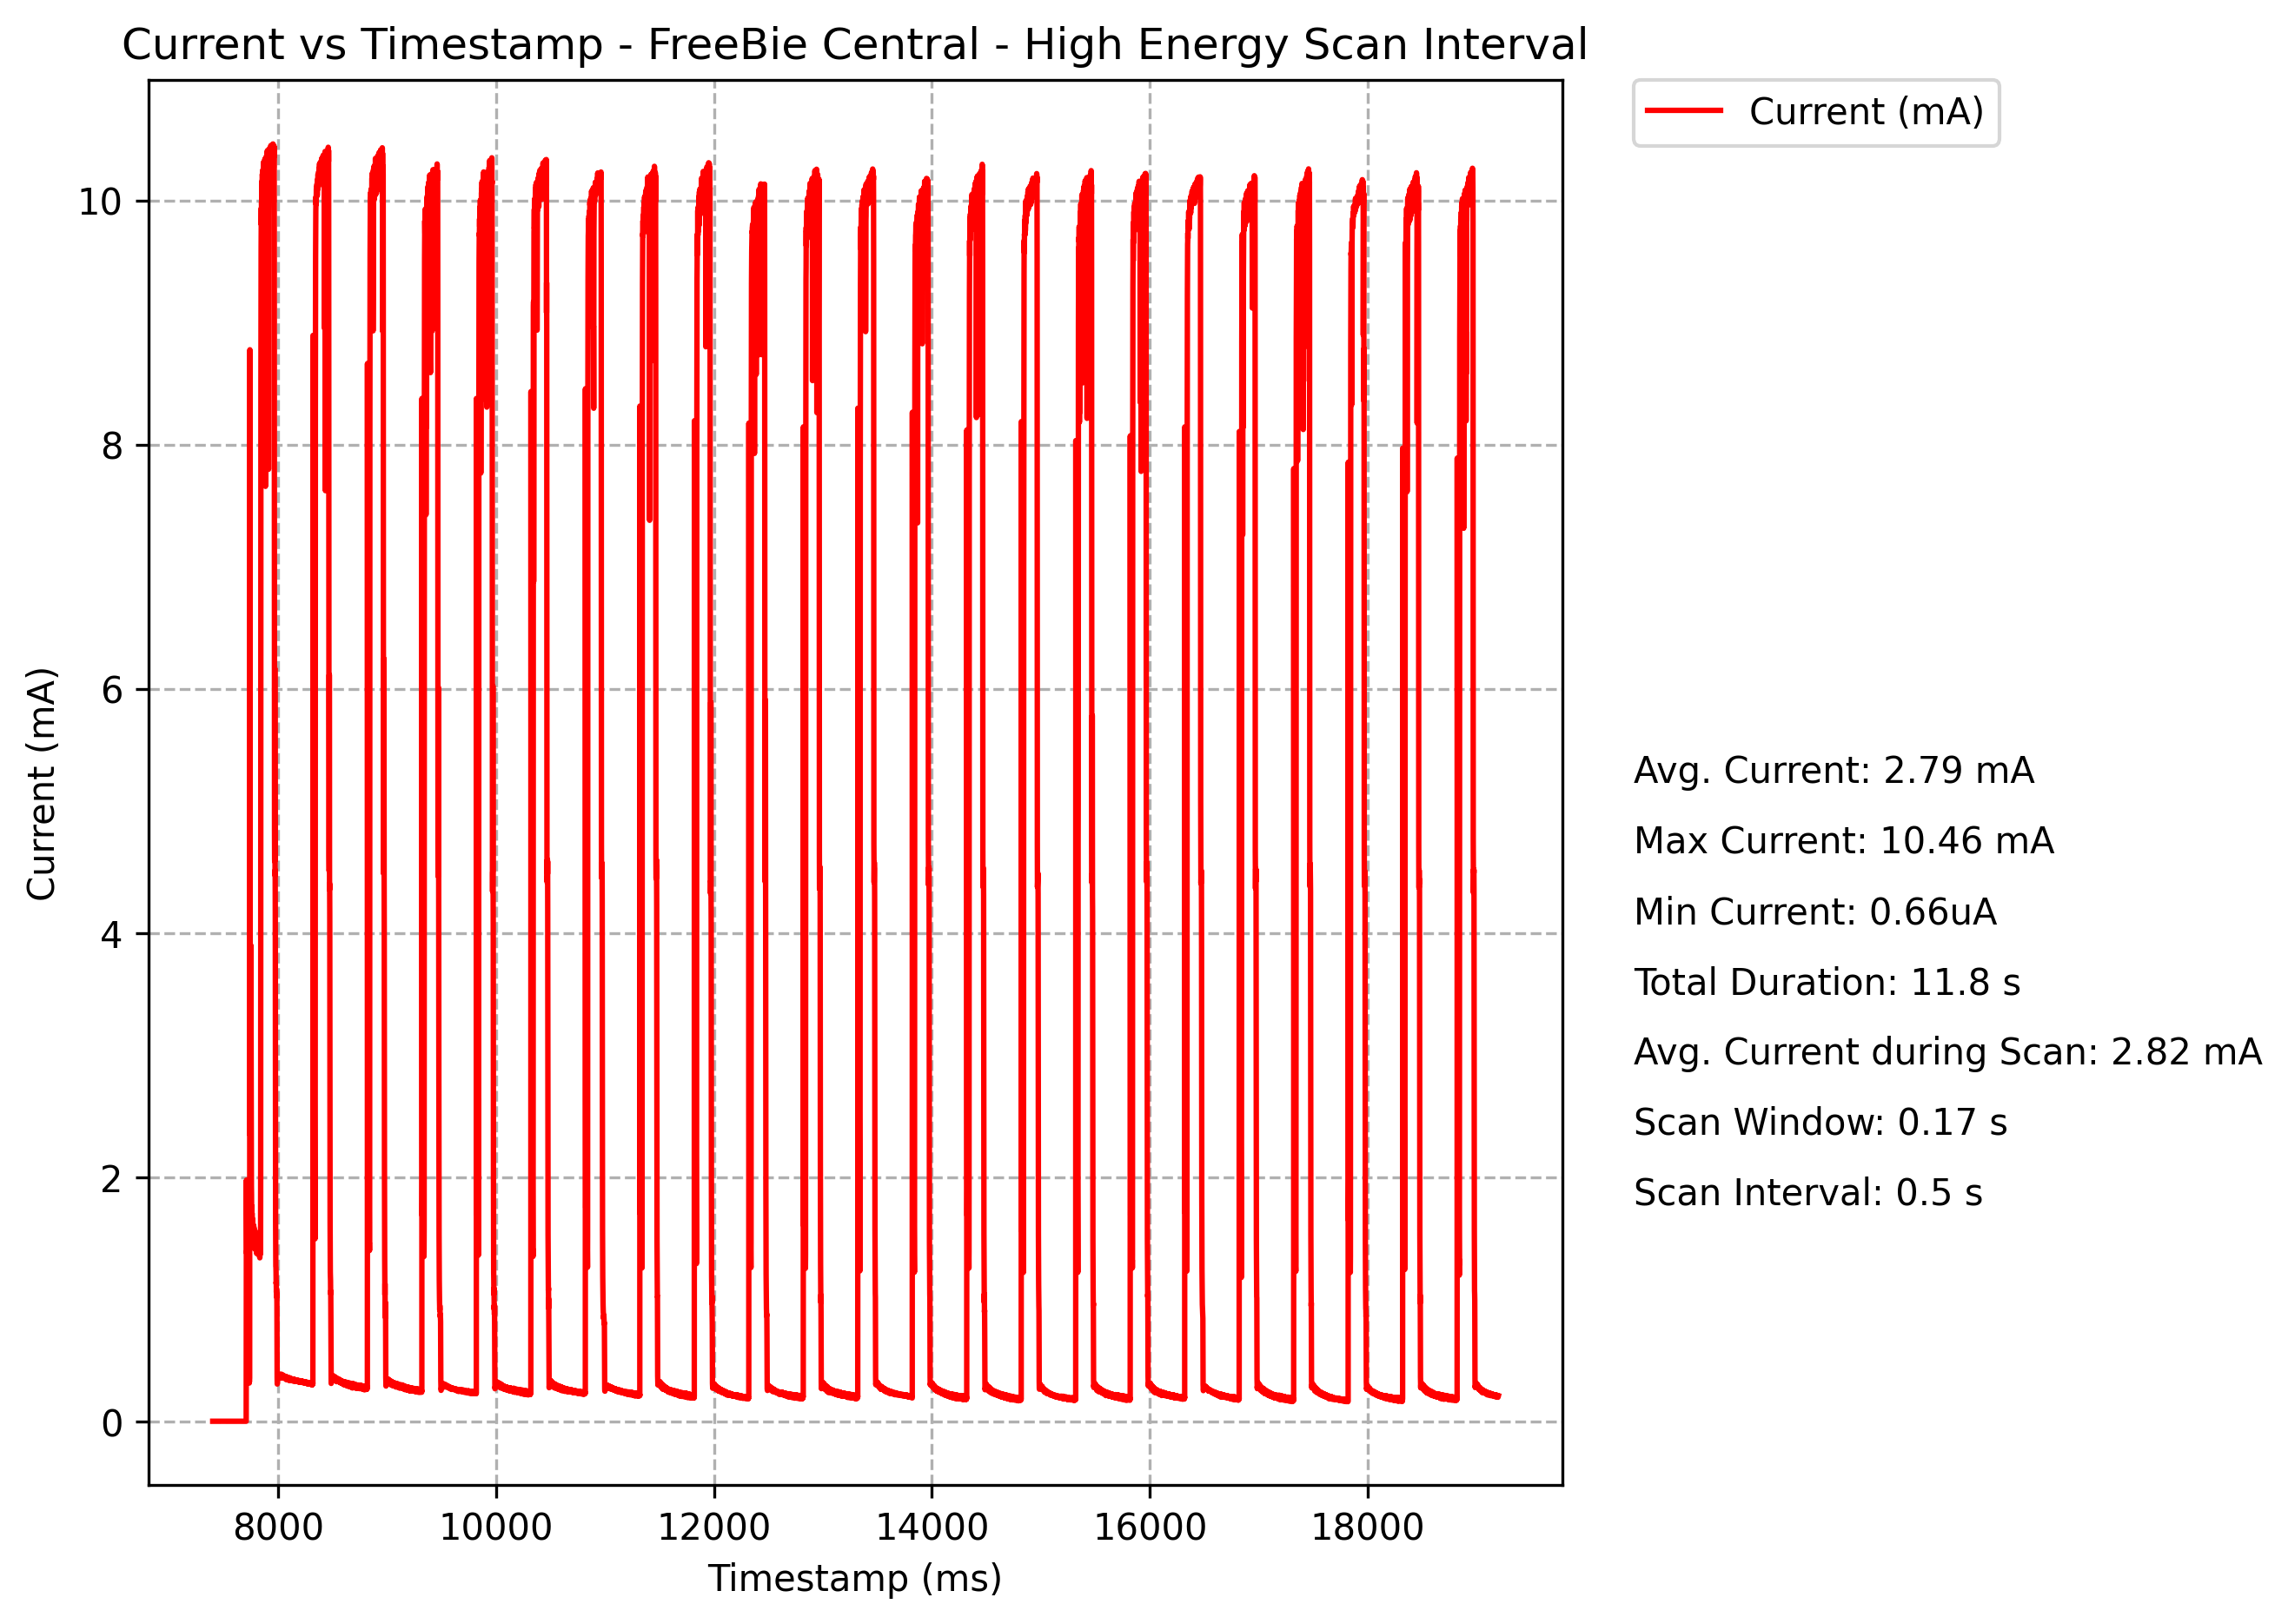
\includegraphics[width=\linewidth]{chapters/Results/Current vs Timestamp - FreeBie Central High.png}
        \caption{FreeBie High- Central}
        \label{fig:freebie_high_central}
    \end{subfigure}\hfill
    \begin{subfigure}{0.45\linewidth}
        \centering
        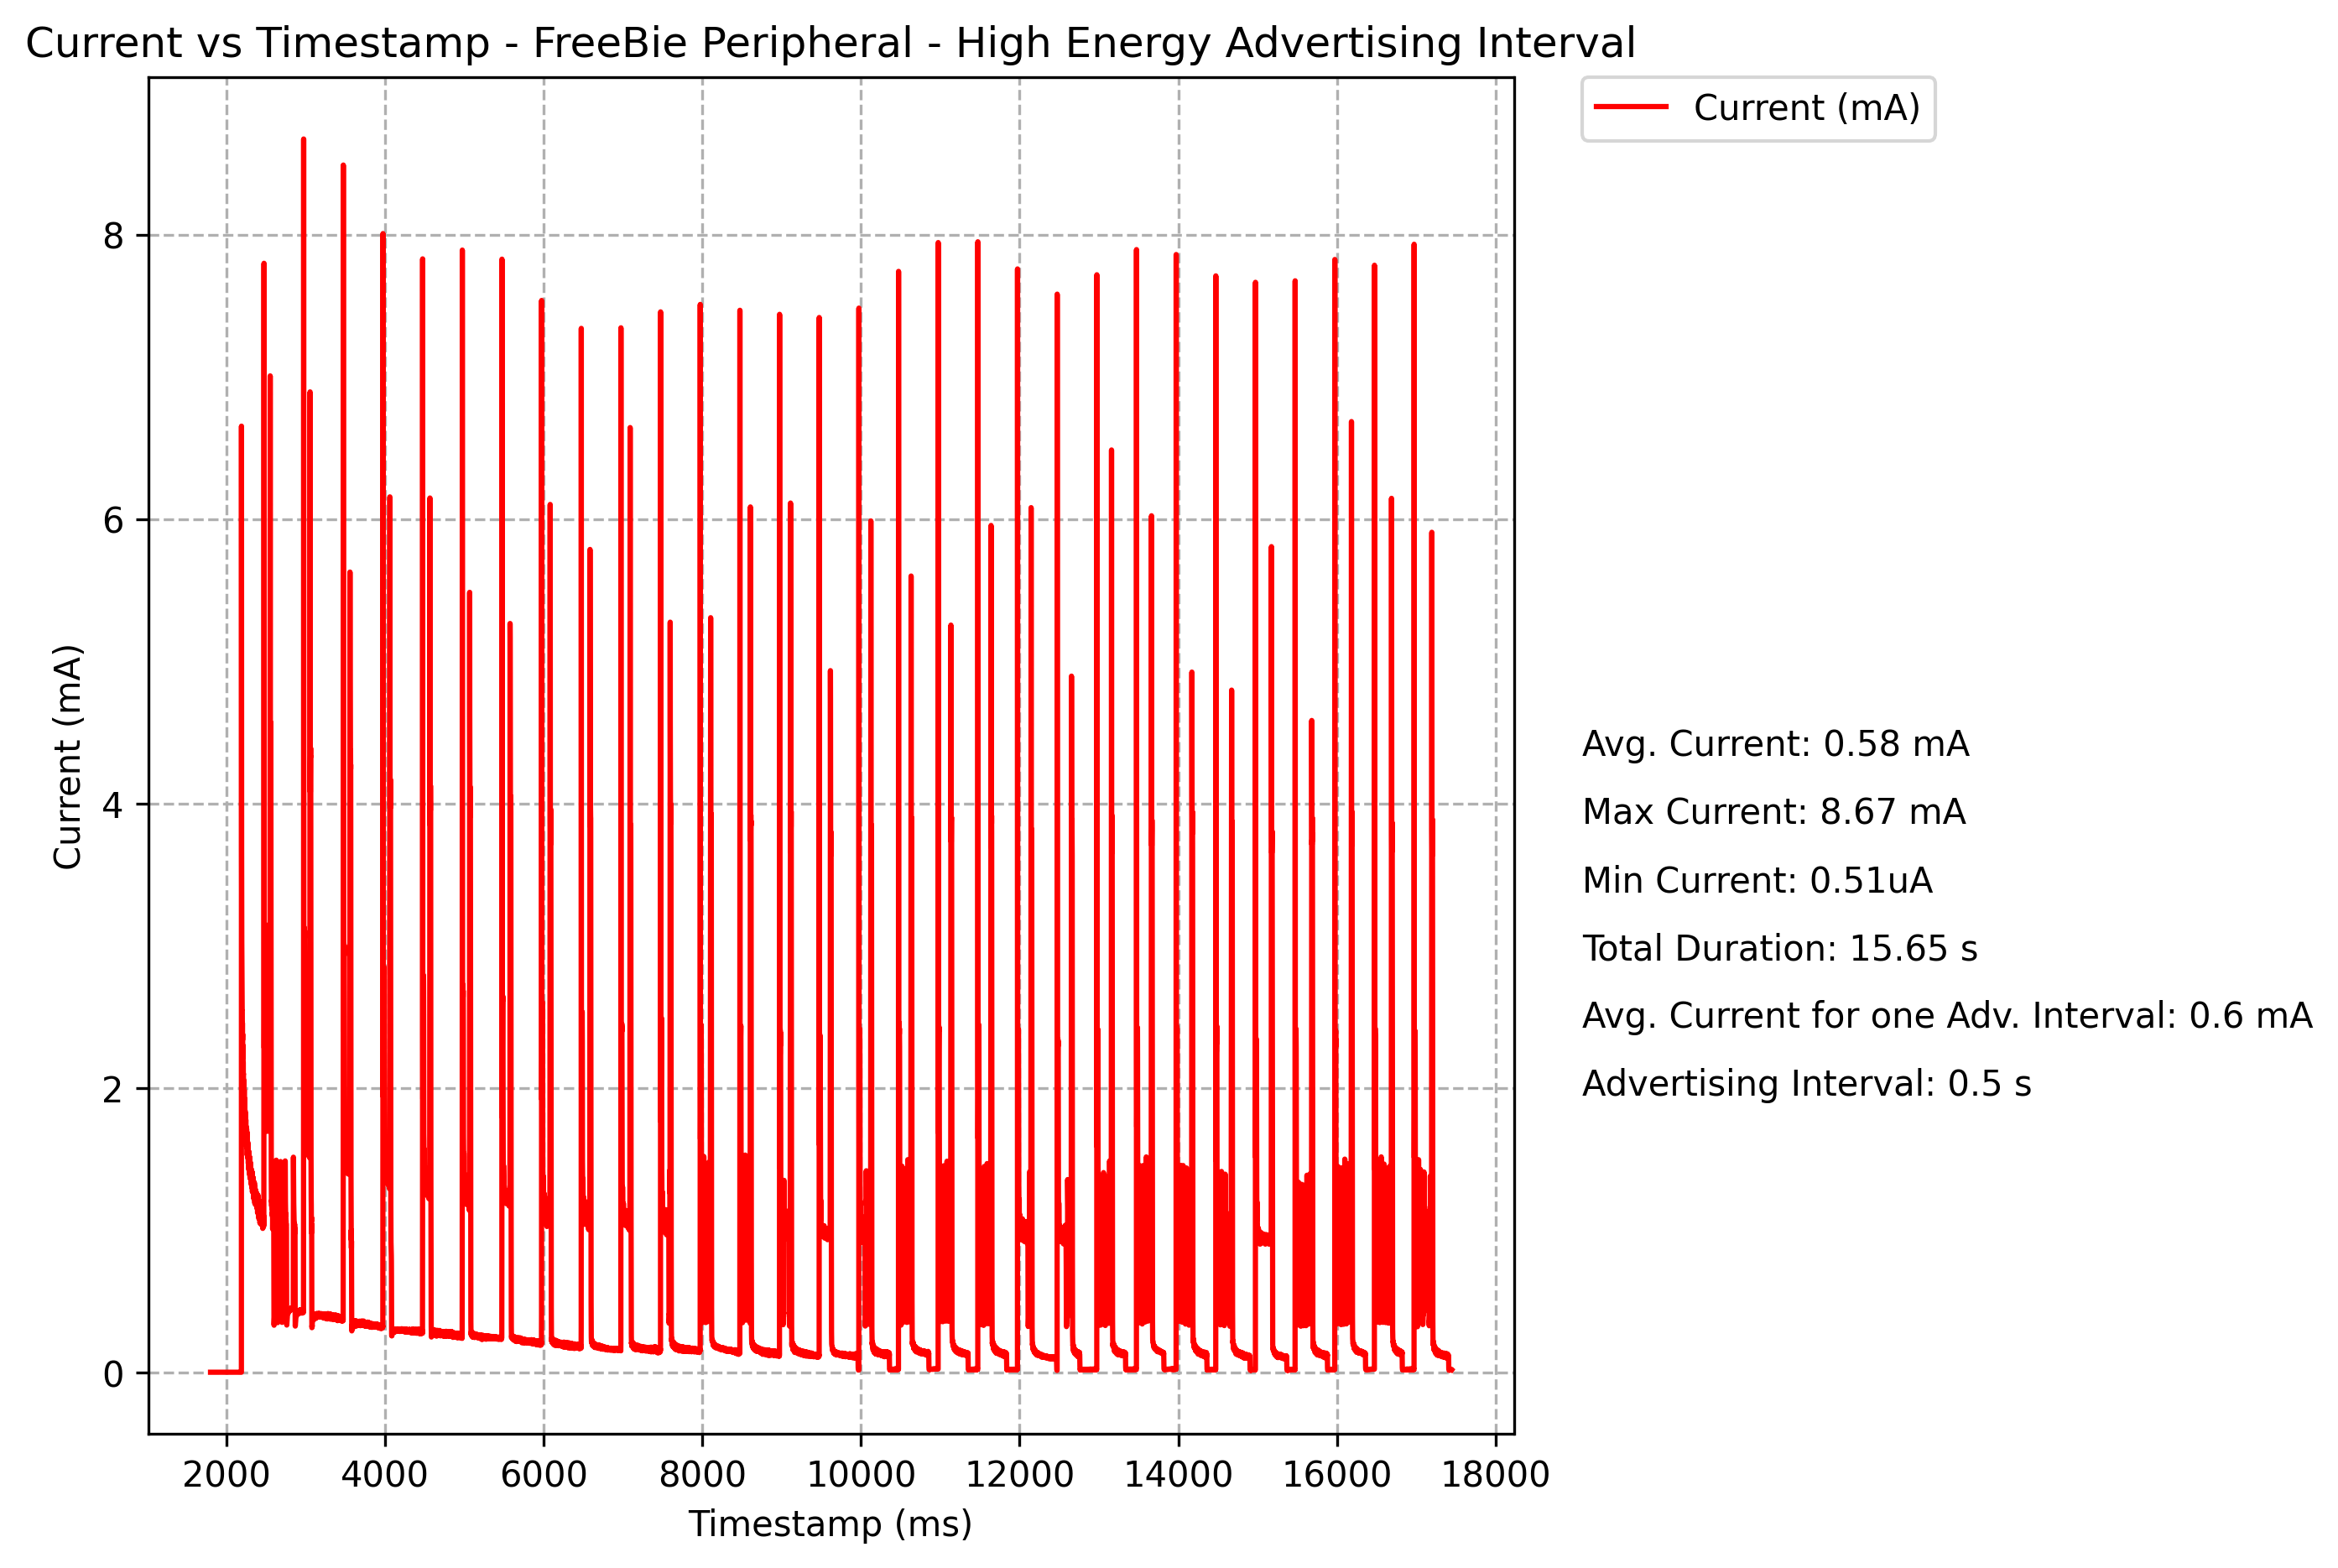
\includegraphics[width=\linewidth]{chapters/Results/Current vs Timestamp - FreeBie Peripheral High.png}
        \caption{FreeBie High - Peripheral}
        \label{fig:freebie_high_peripheral}
    \end{subfigure}
    \caption{Current measurement in idle state without connection establishment for different configurations of reference FreeBie system.}
    \label{fig:current_freebie}
\end{figure}
\begin{table}[t]
\centering
\begin{tabular}{|c|cc|}
\hline
 &
  \multicolumn{2}{c|}{\textit{\textbf{\begin{tabular}[c]{@{}c@{}}Average Current measured\\ in mA\end{tabular}}}} \\ \cline{2-3} 
\multirow{-2}{*}{\textit{\textbf{\begin{tabular}[c]{@{}c@{}}Configuration\\ Name\end{tabular}}}} &
  \multicolumn{1}{c|}{\textit{\textbf{Central}}} &
  \textit{\textbf{Peripheral}} \\ \hline
\cellcolor[HTML]{32CB00}Low    & \multicolumn{1}{c|}{\textit{1.77}} & 0.07 \\ \hline
\cellcolor[HTML]{FFCB2F}Medium & \multicolumn{1}{c|}{\textit{2.78}} & 0.16 \\ \hline
\cellcolor[HTML]{FD6864}High   & \multicolumn{1}{c|}{\textit{2.85}} & 0.6  \\ \hline
\end{tabular}
\caption{Average current measurement using the experimental setup in Section \ref{sec:experimental_setup} for each of the reference system configuration.}
\label{tab:avg_current_freebie}
\end{table}

\noindent Time series voltage measurement plots were generated for each configuration using the same experimental setup discussed in Section \ref{sec:experimental_setup}, as shown in Figure \ref{fig:voltage_freebie}. These plots capture connection establishment during periodic BLE events, with the device entering a sleep state between events, as evidenced by the \(\text{V}_\text{DD\_MCU}\) plot for both Central and Peripheral sides.
\vspace{1\baselineskip}

\noindent Additionally, current trend measured for each BLE configuration in both end devices, as plotted in Figure \ref{fig:current_freebie}, facilitated our comparative energy and power analysis. Then the average current required for BLE connection attempts under various configurations was calculated as illustrated in Table \ref{tab:avg_current_freebie}. 

\subsection{Experimental Setup}
The experimental setup used in this study for comparative assessment is identical to the one stated in Section \ref{sec:experimental_setup}. The experiment recorded the first connection setup time since boot-up for both the CardioSync system and the reference system separately. The measurement of sensor read time is also recorded in the context of the CardioSync system. The experiment was conducted a total of 20 times using the CardioSync device. In the context of the reference system, the experiment is iterated six times for each of the three distinct BLE configurations.
\vspace{1\baselineskip}

\noindent After data collection, the quantification of energy consumption becomes a focal point. The computation of energy expended by the device during each experiment, leading up to connection establishment, is achieved using the formula: \[\text{E(Joules)} = \text{V} \times I_\text{avg} \times T_{\text{Conn}}\].

\noindent The average current $I_\text{avg}$ is measured during distinct phases for both devices, the average voltage supply is 2.6 Volts ($\text{V}$) and $T_\text{Conn}$ corresponds to the time taken to establish a BLE connection since boot up of the device. 
\vspace{1\baselineskip}


\subsection{Connection Setup Time Comparison}
\begin{figure}[t]
    \centering
    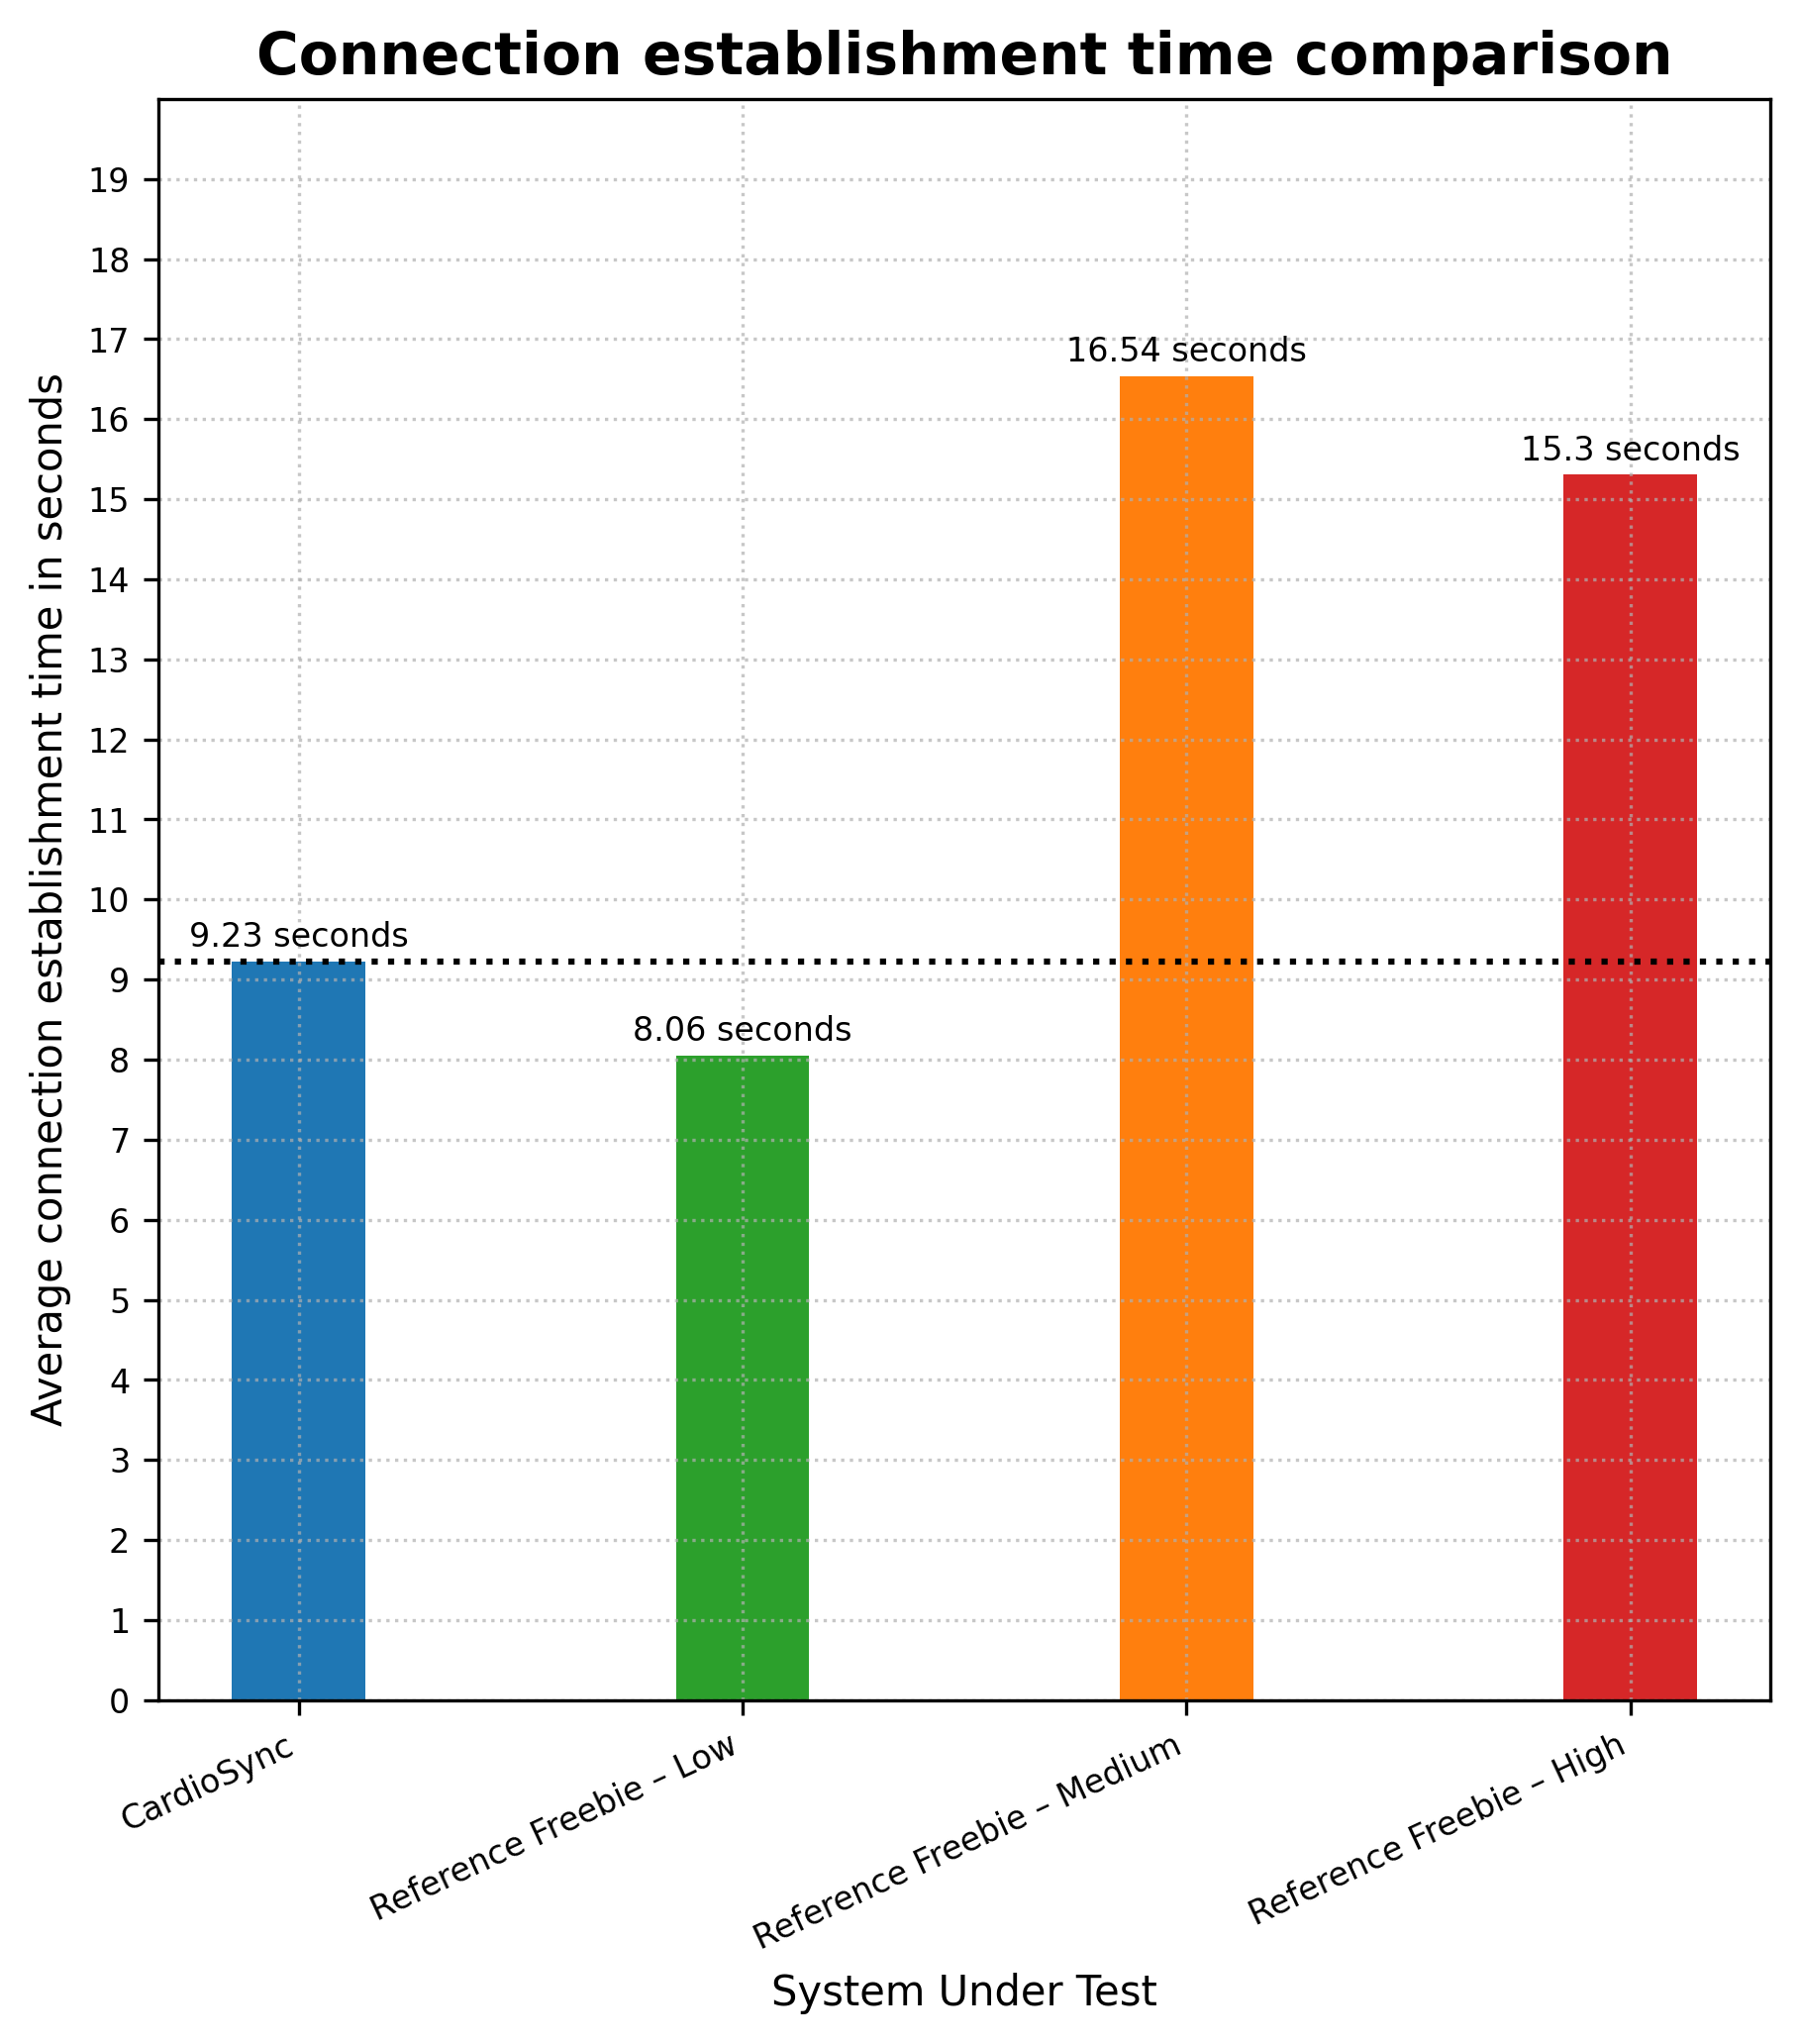
\includegraphics[width=0.7\linewidth]{chapters/Results/Connection_time_comparison.png}
    \caption{Comparison of average BLE connection establishment time for each system.}
    \label{fig:conn_time_comp}
\end{figure}


The bar plot in Figure \ref{fig:conn_time_comp} graphically represents the average connection duration across different systems. Though CardioSync exhibits a slightly longer average connection time compared to the low configuration of the reference FreeBie system, this distinction remains negligible. In contrast, juxtaposing CardioSync with Freebie Medium and FreeBie High configurations reveals a notable improvement in connection efficiency. Impressively, CardioSync achieves an average connection time \textbf{1.79 times faster than FreeBie medium and 1.65 times faster than FreeBie high}.
\vspace{1\baselineskip}

\noindent These insights offer valuable perspectives when considering practical real-world scenarios in the specific contexts chosen to represent the FreeBie reference systems:

\begin{itemize}
    \item \textbf{Limited-Energy Scenario (FreeBie Low):} CardioSync's connection time efficiency, though slightly longer, positions it as a promising solution for scenarios with stringent energy constraints.
    
    \item \textbf{Balanced-Energy Scenario (FreeBie Medium):} CardioSync's significantly faster connection time underscores its potential for enhancing user experiences in fitness tracking devices, where both energy resources and connection efficiency are crucial.
    
    \item \textbf{Abundant-Energy Scenario (FreeBie High):} CardioSync's impressive speed advantage makes it well-suited for scenarios prioritising connection efficiency due to surplus energy availability.
\end{itemize}


\subsection{Energy Consumption Comparison}
\begin{figure}[t]
    \centering
    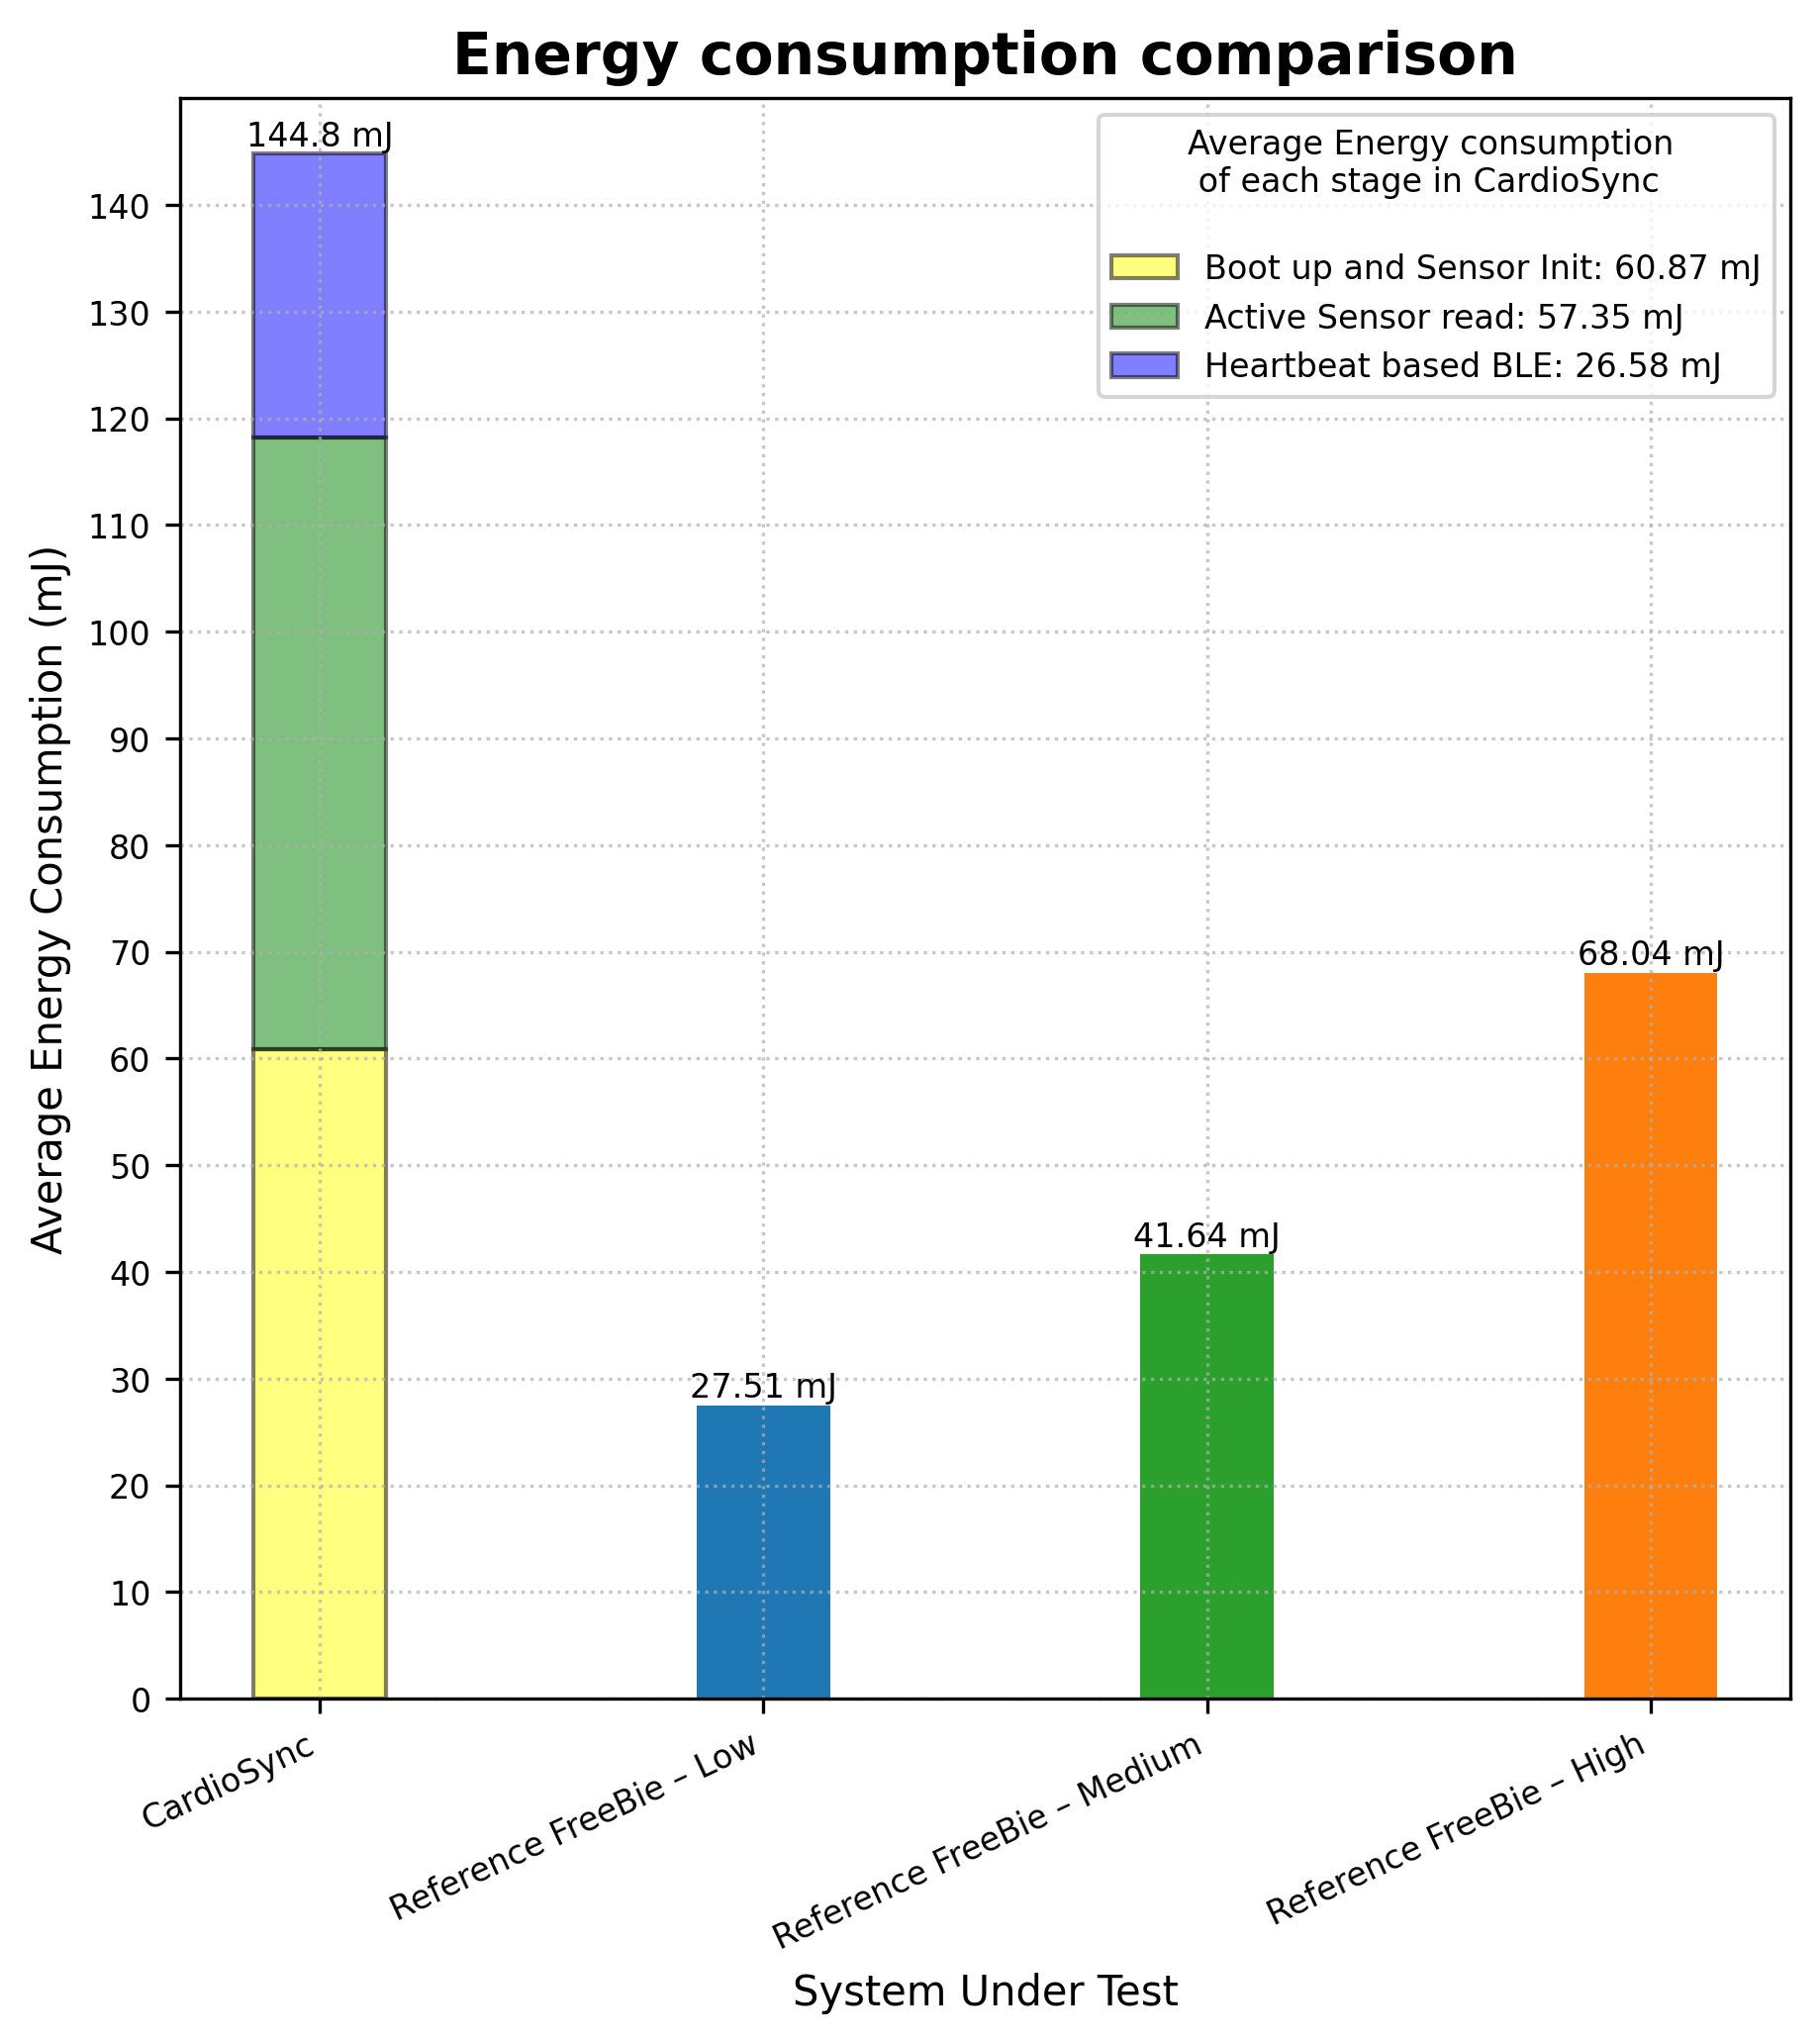
\includegraphics[width=0.7\linewidth]{chapters/Results/Energy_comparison.png}
    \caption{Comparison of average energy consumed till connection setup for each system}
    \label{fig:energy_comp}
\end{figure}

\noindent The bar chart depicted in Figure \ref{fig:energy_comp} provides an illustrative view of the average energy expended to establish a connection for each system. Notably, CardioSync records an average energy consumption of 144.8 mJ, encompassing the cumulative energy consumption from boot-up, sensor initialisation, the "Read and Synchronise" phase, and the "Sleep and Synchronise" phase. The partitioning of this energy consumption into distinct phases is depicted in the bar chart, showcasing the distribution of energy allocation for comprehensive insight. As anticipated, the "Sleep and Synchronise" consumes energy of 26.58 mJ, which is more similar to the energy expended by Naive FreeBie design with a low configuration. This confirms that sensor initialisation and active sensor reading, which employs a polling method, are active energy-consuming phases. In contrast, the reference FreeBie systems exhibit significantly lower energy expenditures—27.51 mJ for FreeBie Low, 41.64 mJ for FreeBie Medium, and 68.04 mJ for FreeBie High.
\vspace{1\baselineskip}

\noindent Comparison of these results reveals that CardioSync consumes notably more energy compared to the reference FreeBie systems. This distinction is particularly evident when compared to FreeBie Low, where CardioSync's energy consumption is around \textbf{5.263 times higher}. Similarly, when contrasted with FreeBie Medium and FreeBie High, CardioSync's energy consumption is \textbf{3.48 and 2.13 times higher}, respectively.
\vspace{1\baselineskip}

\noindent This observed energy disparity aligns with the inherent characteristics of CardioSync, where the integration of the MAX30102 sensor introduces increased energy consumption as a trade-off for improved synchronisation and connection efficiency. Also in the context of the scenarios chosen for the FreeBie reference systems:

\begin{itemize}
    \item \textbf{Limited-Energy Scenario (FreeBie Low):} CardioSync's higher energy consumption aligns with scenarios where energy constraints are paramount, raising questions about its feasibility in such settings.
    
    \item \textbf{Balanced-Energy Scenario (FreeBie Medium):} In scenarios like fitness trackers, where energy resources are limited, the energy efficiency of CardioSync becomes a crucial consideration for extended device functionality. This is particularly important when connection setups fail for extended periods, despite CardioSync demonstrating its ability to operate with intermittent power sources.
    
    \item \textbf{Abundant-Energy Scenario (FreeBie High):} While CardioSync's energy consumption is higher, its speed advantage suggests suitability for scenarios where connection efficiency is prioritised due to surplus energy availability.
\end{itemize}

% \subsection{Power Comparison}
% \begin{figure}[t]
%     \centering
%     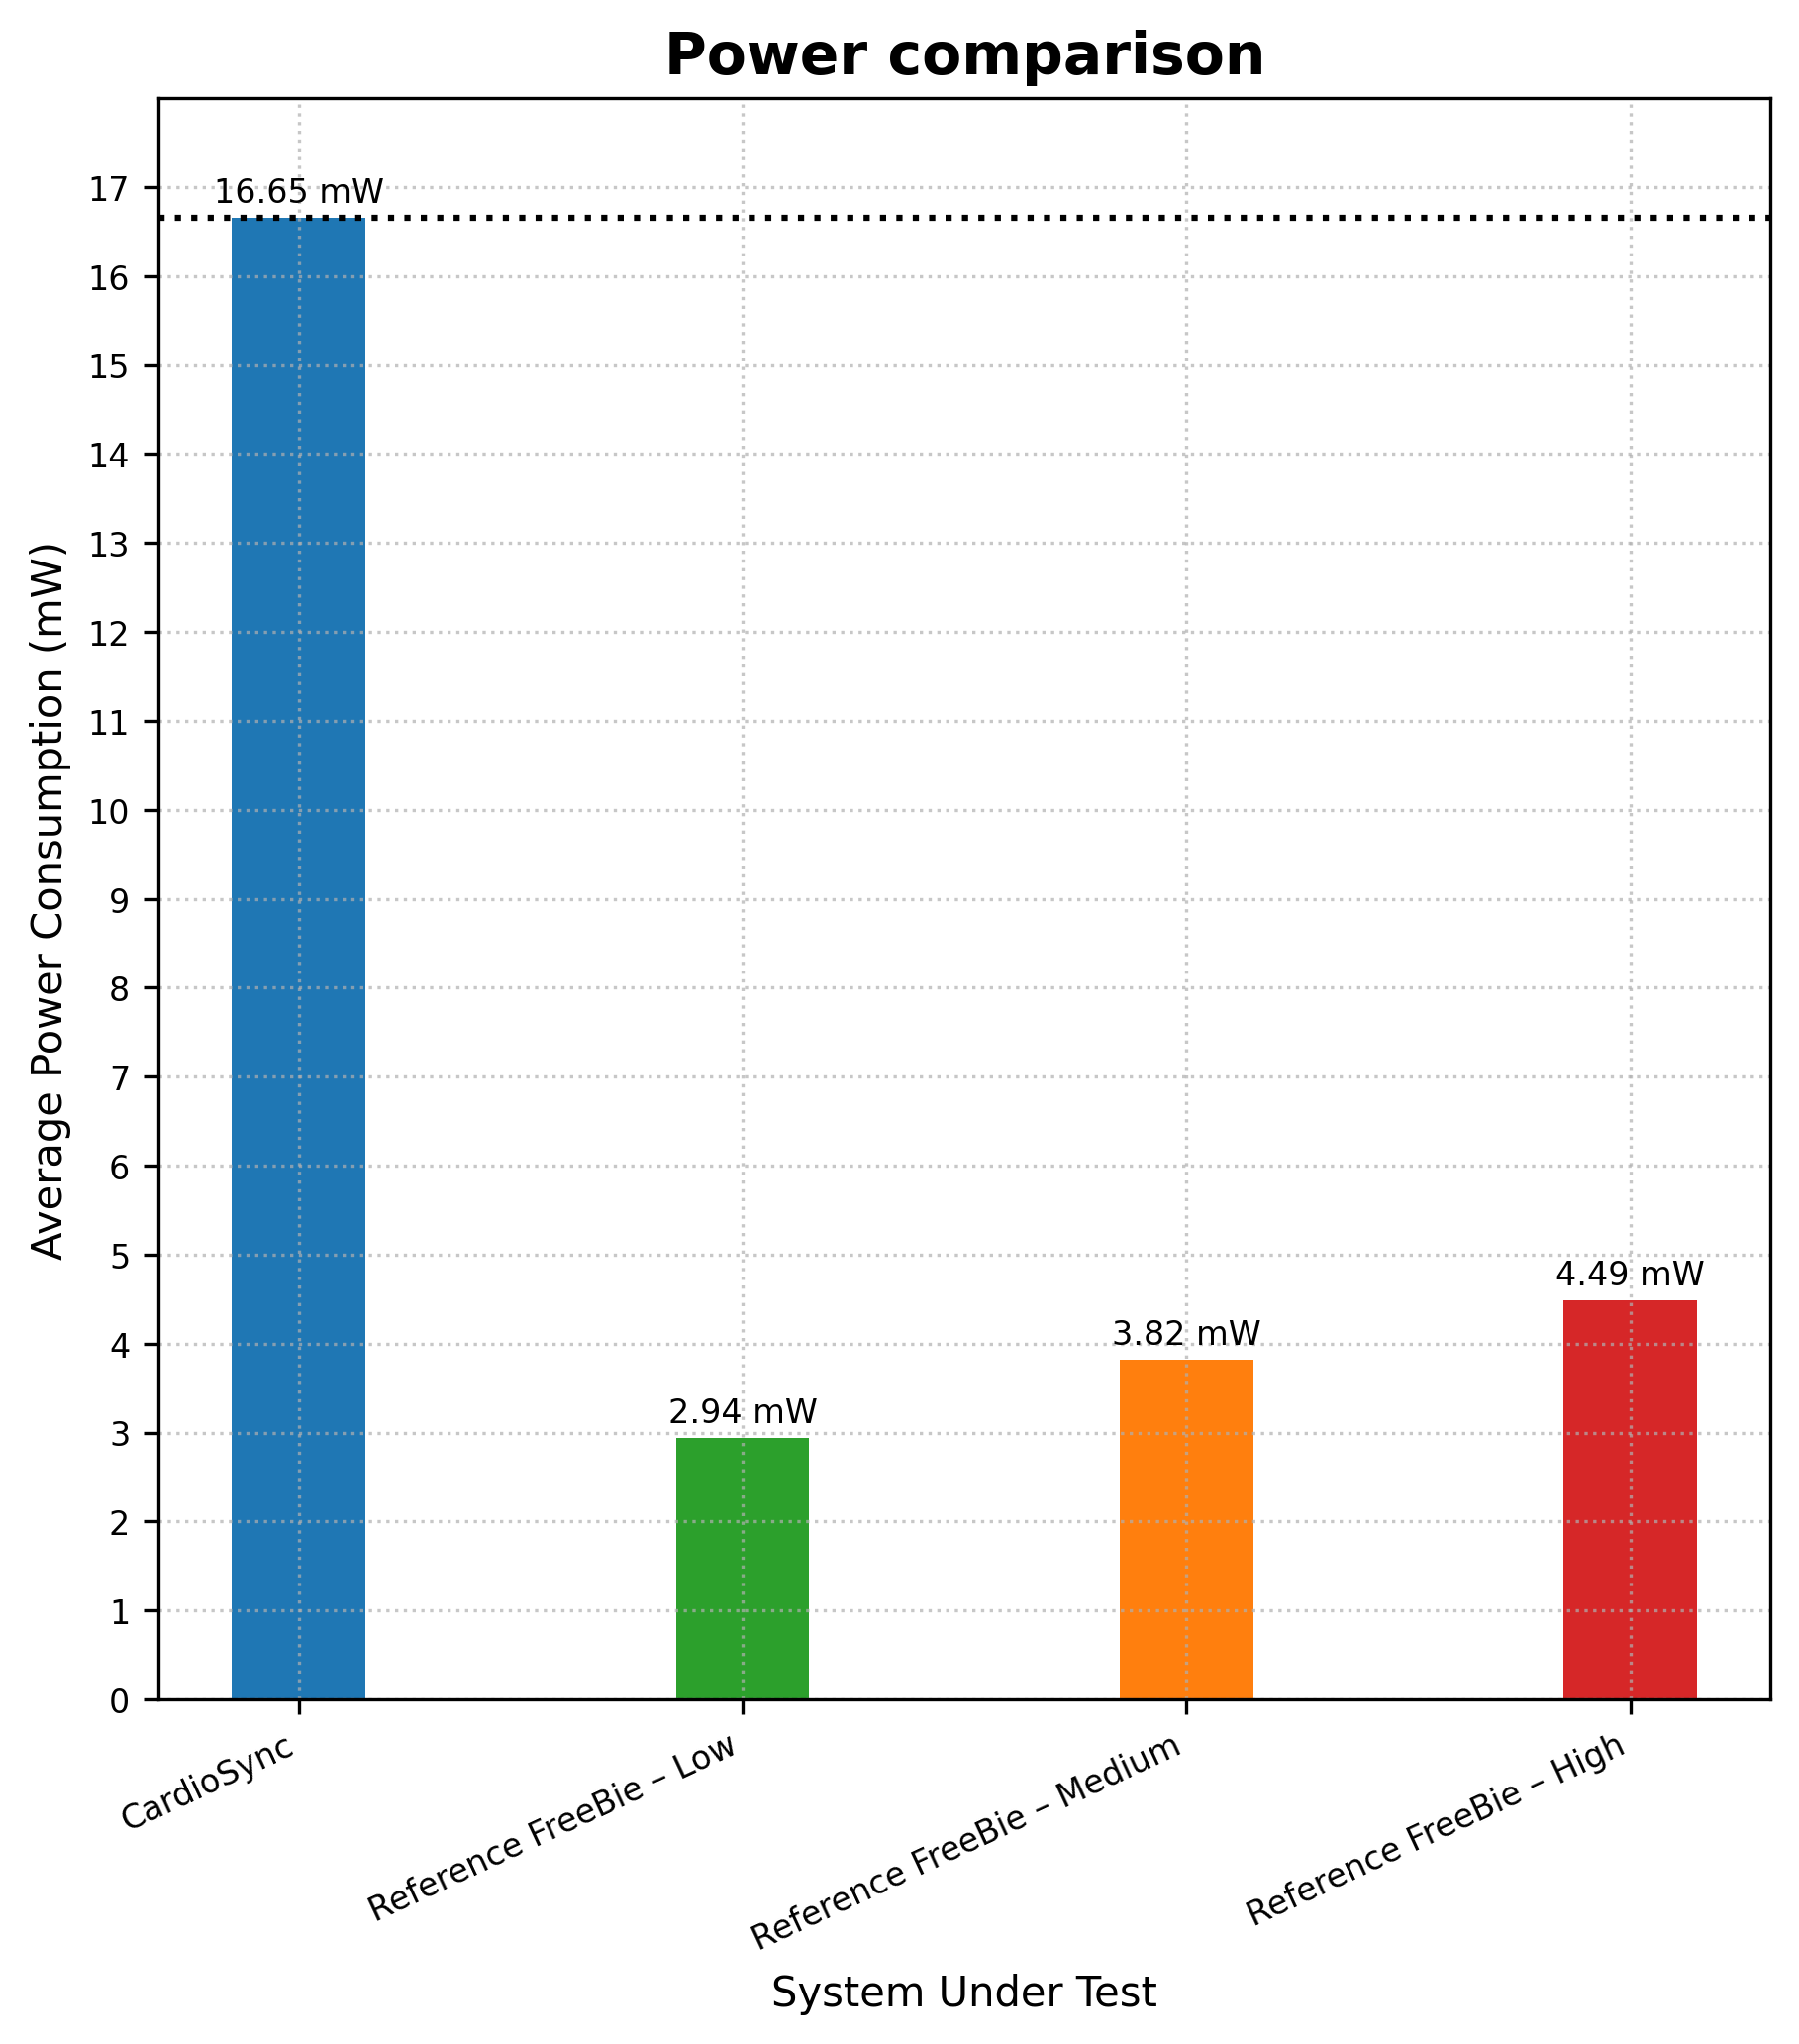
\includegraphics[width=0.7\linewidth]{chapters/Results/Power_comparison.png}
%     \caption{Bar plot showing Average power consumed till connection setup for each system for comparison}
%     \label{fig:power_comp}
% \end{figure}

% \noindent The bar chart depicted in Figure \ref{fig:power_comp} offers a visual representation of the average power expended to establish a connection for each system. Comparing these outcomes underscores that CardioSync consumes significantly more power when compared to the reference FreeBie systems. In comparison to FreeBie Low, CardioSync's power consumption is \textbf{5.66 times higher}. Similarly, in relation to FreeBie Medium and FreeBie High, CardioSync's power consumption is \textbf{4.36 and 3.70 times higher}, respectively. This power discrepancy mirrors the energy consumption pattern observed earlier and is congruent with the inherent trade-offs of the CardioSync system.


\subsection{Understanding Connection Setup Vs. Power}
\begin{figure}[t]
    \centering
    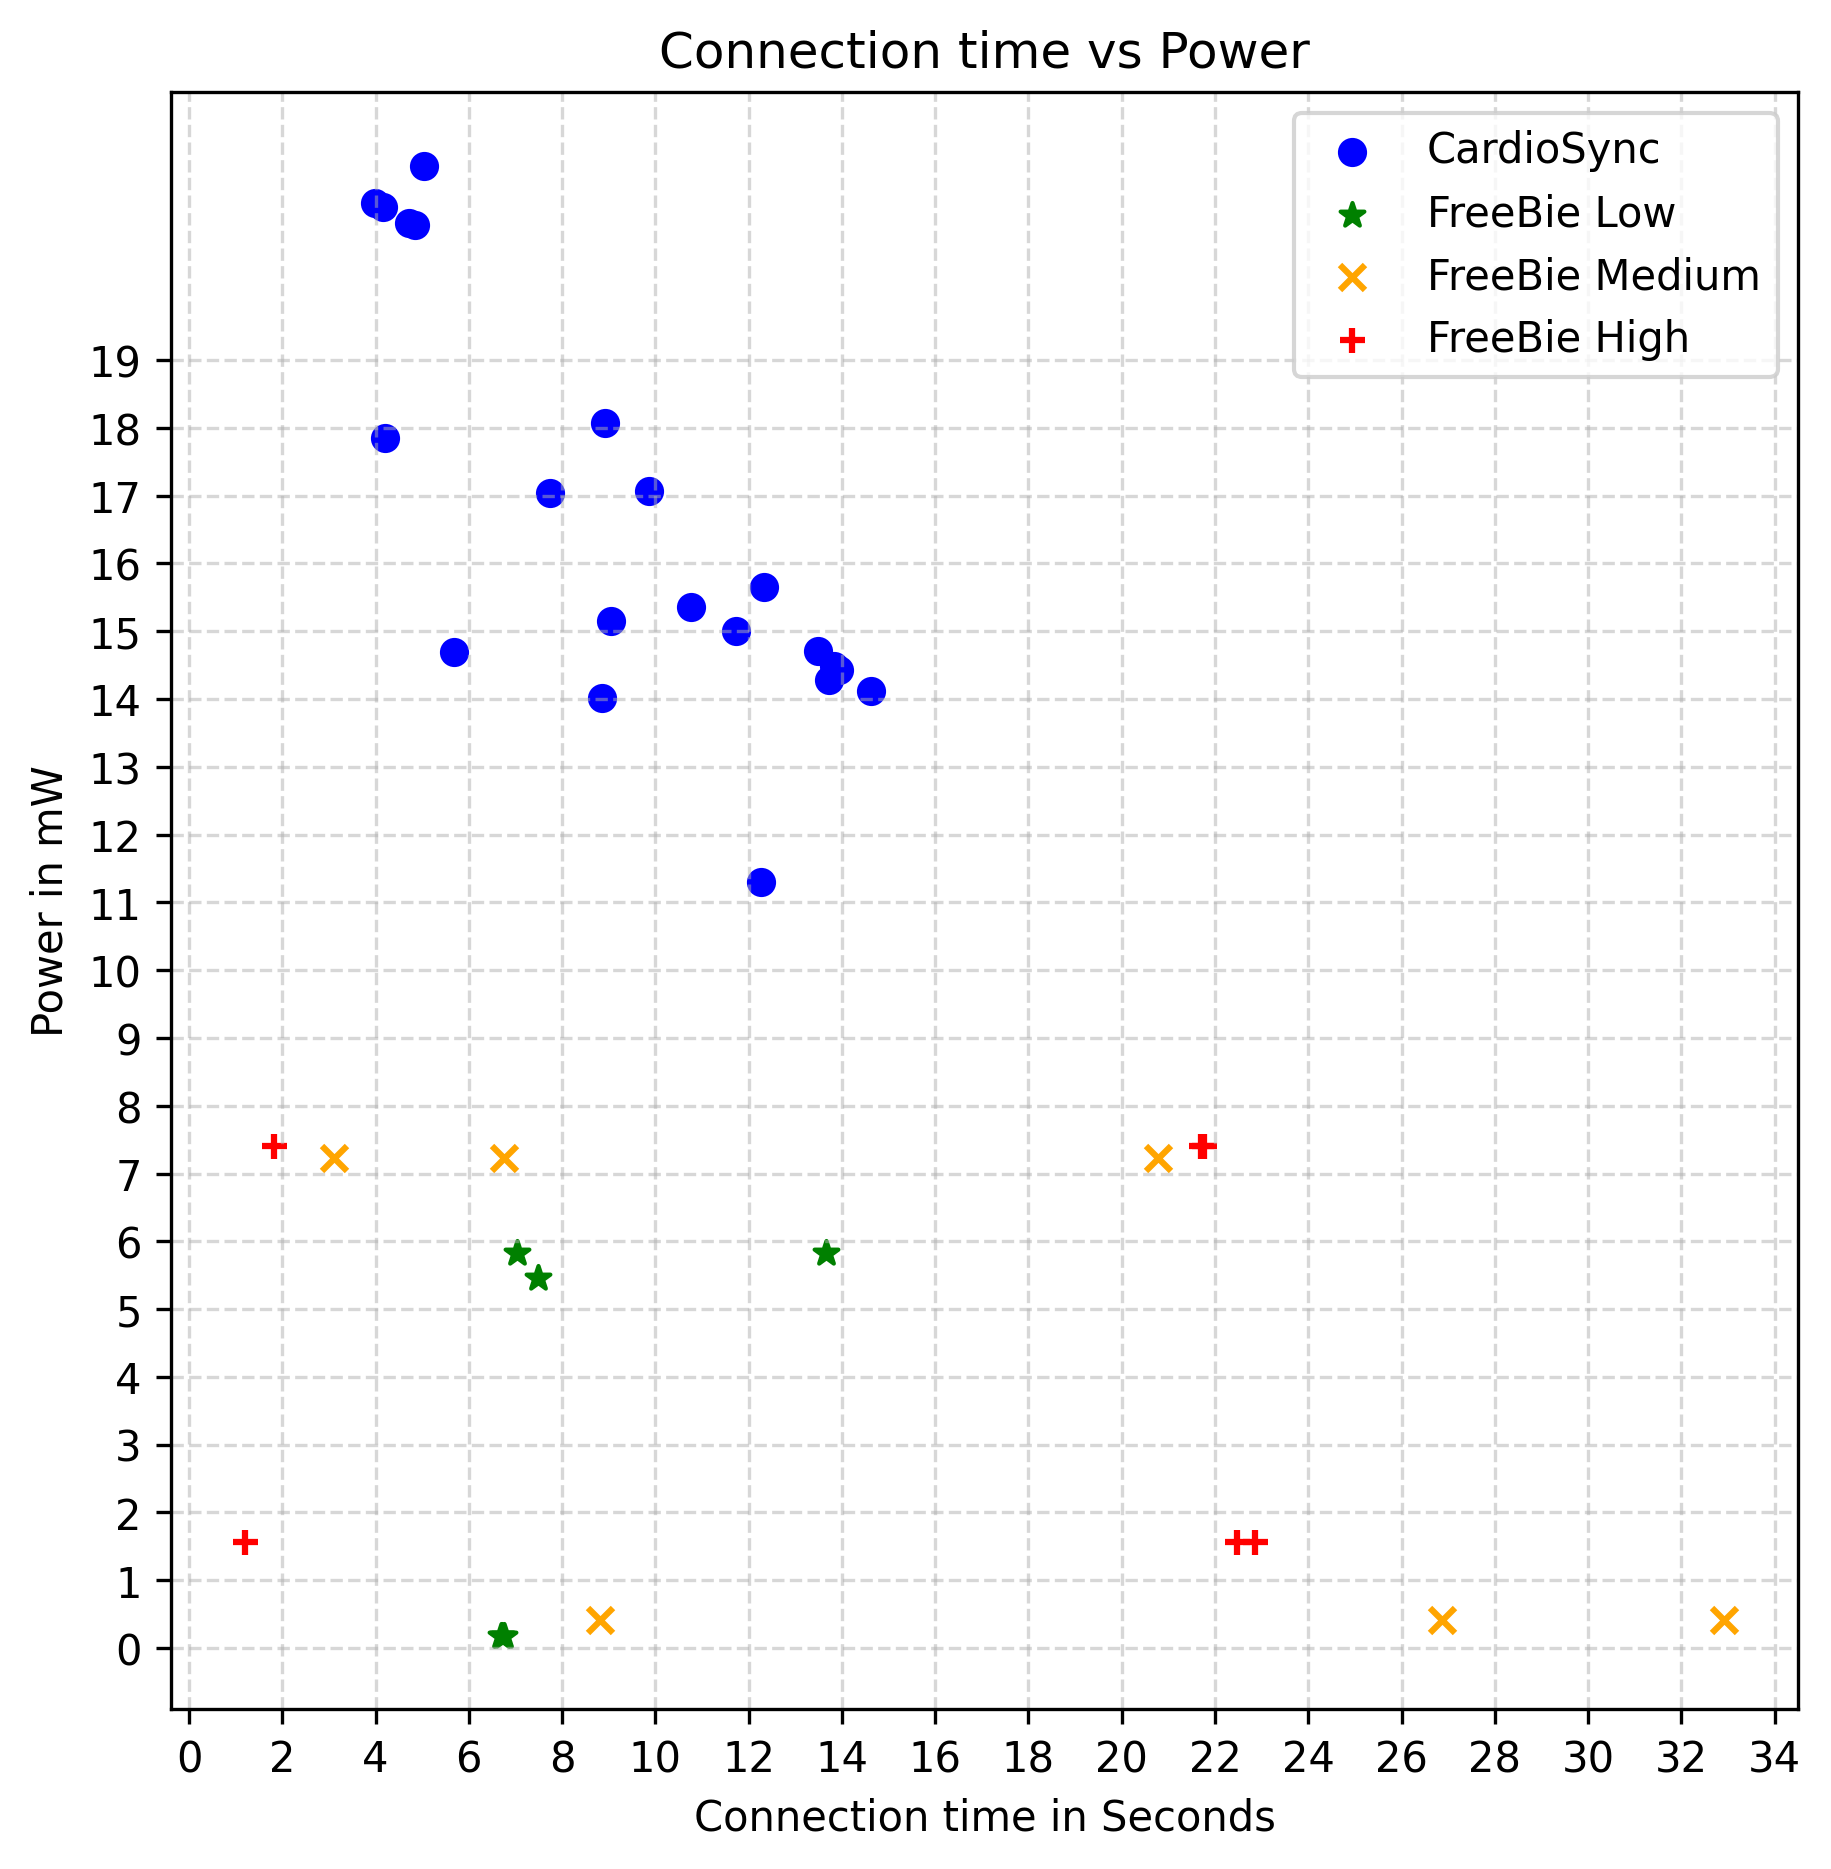
\includegraphics[width=0.7\linewidth]{chapters/Results/Scatter_plot.png}
    \caption{Scatter plot showing Connection time Vs. Power}
    \label{fig:scatter_conn_power}
\end{figure}

\noindent Figure \ref{fig:scatter_conn_power} presents an insightful juxtaposition of connection time against power consumption for both the CardioSync and reference FreeBie systems. Notably, the distribution of experimental data points for the CardioSync system predominantly converges in the upper left quadrant of the graph. In contrast, the scatter plot depicting the reference FreeBie system showcases a more dispersed arrangement of data points, spanning across the lower half of the graph.
\vspace{1\baselineskip}

\noindent This disparity in the distribution of data highlights a pivotal distinction between the two systems. While the CardioSync system exhibits greater power consumption, it consistently achieves expedited connection times. In contrast, the reference FreeBie system, characterised by its asynchronous nature, demonstrates a wider range of connection times. This inconsistency in connection times, despite relatively lower power consumption, highlights the challenges inherent in achieving synchronisation within the battery-less FreeBie architecture.
\vspace{1\baselineskip}

\noindent In essence, the scatter plot serves as a visual testament to the trade-offs between power consumption and connection time. The CardioSync system, which has denser data points in the upper left quadrant, is an example of the potential advantages of utilising external synchronisation mechanisms to achieve consistent and effective connection times in a battery-free context.


\section{Discussion of Key Findings}
In this section, we explore the implications and insights stemming from the comparative analysis between the CardioSync framework and the reference FreeBie system, shedding light on their performance and potential trade-offs.

\begin{itemize}
    \item \textbf{Power and Energy Efficiency:} CardioSync demonstrated higher connection time efficiency, counterbalanced by increased power and energy consumption. This is due to the intentional inclusion of the MAX30102 sensor for synchronisation, which inherently demands additional energy. It's worth noting that the energy spent to establish a synchronised reconnection in case of connection timeouts is significantly lower in CardioSync compared to naive reference FreeBie systems.

    \item \textbf{Connection Time and Synchronisation:} CardioSync consistently achieved reduced connection times, while the reference FreeBie system exhibited a wider range of connection times, reflecting its asynchronous nature. Importantly, the readings from the reference system are after intentional synchronisation. Without this, the reference system's BLE advertising and scanning intervals remain asynchronous, rendering it unable to establish connections. In contrast, CardioSync achieves synchronisation effortlessly.

    \item \textbf{Trade-Offs and Implications:} CardioSync's higher energy usage, resulting in improved connection times, introduces trade-offs to consider in real-world applications. The dispersed connection times in the reference FreeBie system highlight the difficulty of achieving synchronisation.

\end{itemize}

\noindent In summary, the detailed evaluation of CardioSync against the reference FreeBie system aligns strategically with our research objectives and validates our research goals, effectively enhancing the discourse and possibilities within the battery-less domain.